
%==============================================================================%
% A PhD thesis template, based on LaTeX memoir class rather than the standard  %
% book class, as memoir offers many additional configuration options.          %
%                                                                              %
% For documentation on the memoir class, and other packages, see:              %
%                                                                              %
%   http://www.ctan.org/search/                                                %
%                                                                              %
% Dave Green --- MRAO --- 2016 September (Version 1.12)                        %
%==============================================================================%
% load the memoir class with basic options ...
%
\documentclass[a4paper,11pt,oneside,extrafontsizes,oldfontcommands]{memoir}
%

% load the thesis package, which sets various options for the memoir
% package, loads other packages (e.g. setting up fonts), and sets up
% various commands ...
%
% note: you will have to edit thesis.sty if you want to change things ...
%
\usepackage{thesis}
%
% other settings...
%
%\listfiles     % uncomment if needed for debugging ...
%------------------------------------------------------------------------------%
% For limited processing, list (with commas) selected files to process...
%
%\includeonly{CHAP-1/chapter1,APP-A/appendixa}
%
\begin{document}
%==============================================================================%

%------------------------------------------------------------------------------%
\mainmatter
\pagestyle{empty}
%
% titlepage ...
%
\ifpdf
  \pdfbookmark[0]{Titlepage}{title}{}
\fi
%
% note: include adjustment of baseline to ensure it looks
%       sensible if it is more than one line long,
%
\begin{center}
 \qquad\\[10mm]
 {\renewcommand\baselinestretch{1.2}\Huge\textbf{
%
% if more than one line, use "\\" to start a new line...
%
   Dave Green's thesis template
%
 }\par}
 \qquad\\[50mm]
 {\LARGE Andrew James Strange}\\[10mm]
 {\large School of Physics and Astronomy}\\[10mm]
 
\includegraphics[width=50mm]{UniOfManchesterLogo.png}\\[30mm]
 {\Large 2017 September}\\[10mm]
 {\large A thesis submitted to the University of Manchester \\ for the degree of Master of Science \\ in the Faculty of Engineering and Physical Sciences}
\end{center}

\cleardoublepage

\endinput

%
\pagestyle{plain}
%
% contents ...
%
\setcounter{page}{2}
%
% thesis.sty redefines \baselinestretch for larger line spacings, but
% here do not use this for the table of contents ...
%
\bgroup
\renewcommand{\baselinestretch}{1.0}\normalsize

\tableofcontents

%
% reset to default linespacing ...
%
\vspace{10mm}
\textit{Word Count: 16858}
\egroup

\cleardoublepage

\endinput

%
% thesis.sty redefines \baselinestretch for larger line spacings, but
% here do not use this for the table of contents ...
%
\bgroup
\renewcommand{\baselinestretch}{1.0}\normalsize

\listoffigures

%
% reset to default linespacing ...
%
\egroup

\cleardoublepage

\endinput

%
% thesis.sty redefines \baselinestretch for larger line spacings, but
% here do not use this for the table of contents ...
%
\bgroup
\renewcommand{\baselinestretch}{1.0}\normalsize

\listoftables

%
% reset to default linespacing ...
%
\egroup

\cleardoublepage

\endinput

%
% declaration ...
%
\chapter*{ABSTRACT}

\addcontentsline{toc}{chapter}{Abstract}

This dissertation presents a feasibility study on the application of Trigger-Object Level Analysis (TLA) to the search for the Standard Model Higgs boson produced by Vector Boson Fusion (VBF) and decaying to b-quarks, using $4.6$fb$^{-1}$ of proton-proton collision data taken at a centre-of-mass energy of $13$TeV by the ATLAS detector. The VBF process is predicted to be the second largest cross-section process at the Large Hadron Collider, and searches for the VBF produced Higgs decaying to $b\bar{b}$ exploit the characteristic final state topology to select events. TLA refers to the procedure of only storing the jet objects reconstructed at the trigger-level of the ATLAS detector for use in analysis, which permits an increase in the output rate of the detector, as a result of reducing the byte size of the detector readout.

This dissertation suggests that a TLA approach is feasible for the \VBFHBB\ channel. The analysis showed that the behaviour of trigger-level jets was comparable to that of the standard reconstructed jets, and the agreement of the jet kinematic properties could be improved by applying trigger-level calibrations. Simulating the \VBFHBB\ analysis using trigger-level objects resulted in a $20\%$ reduction in the number of final events for the TLA compared to the standard analysis, which shows that the $100\%$ detector output rate increase from the current TLA approach would produce an overall increase in the number of final state events. Select kinematic properties of the \VBFHBB\ final state were studied and shown to demonstrate comparable behaviour between the trigger-level and standard reconstructed objects.

\cleardoublepage

\endinput

\chapter*{Declaration}

\addcontentsline{toc}{chapter}{Declaration}

No portion of the work referred to in the dissertation has been submitted in support of an application for another degree or qualification of this or any other university or other institute of learning.

\cleardoublepage

\endinput

\chapter*{Copyright Statement}

\addcontentsline{toc}{chapter}{Copyright Statement}

The author of this dissertation (including any appendices and/or schedules to this dissertation) owns certain copyright or related rights in it (the "Copyright") and he has given The University of Manchester certain rights to use such Copyright, including for administrative purposes.

Copies of this dissertation, either in full or in extracts and whether in hard or electronic copy, may be made only in accordance with the Copyright, Designs and Patents Act 1988 (as amended) and regulations issued under it or, where appropriate, in accordance with licensing agreements which the University has from time to time. This page must form part of any such copies made.

The ownership of certain Copyright, patents, designs, trademarks and other intellectual property (the "Intellectual Property") and any reproductions of copyright works in the dissertation, for example graphs and tables ("Reproductions"), which may be described in this dissertation, may not be owned by the author and may be owned by third parties. Such Intellectual Property and Reproductions cannot and must not be made available for use without the prior written permission of the owner(s) of the relevant Intellectual Property and/or Reproductions.

Further information on the conditions under which disclosure, publication and commercialisation of this dissertation, the Copyright and any Intellectual Property and/or Reproductions described in it may take place is available in the University IP Policy, in any relevant Dissertation restriction declarations deposited in the University Library, The University Library's regulations and in The University's policy on Presentation of Dissertations

\cleardoublepage

\endinput

%
% thanks ...
%
\chapter*{Acknowledgements}

\addcontentsline{toc}{chapter}{Acknowledgements}

This dissertation has been produced with guidance and support from many people, without which it would not have seen the light of day.

Primarily, I must thank my supervisor Andy Pilkington. His guiding hand and experience over the course of this project has at times been the only thing keeping it on the straight and narrow. I am indebted to his help and his willingness to put up with me over the course of this year, and this work is built around the backbone he provided.

Secondly, thanks to the Manchester Particle Physics group, for providing a terrific environment for work, for all of the guidance and for all of the socialising. Particular mention must go to my colleagues on the ATLAS project; Jacob, Jonathan
, Yaadav and Agni for all of their invaluable experience and assistance throughout the year. Additionally, I must thank Sabah for providing me with his help and knowledge without hesitation when I needed it.

From my time at undergraduate, I must thank all my friends, who while provided encouragement and support from all the myriad of locations around the world they've run off to, and I must thank my undergraduate Director of Studies, Dave Green, for his advice during my time under his watch and for permitting me to use his \LaTeX template.

Finally however, none of this would have occurred were it not for the support of my dad, mum and brother. Their unwavering and tireless support, endless encouragement and motivating prods and willing to put up with whatever inconvenience I could give them carried this work through to its close.

To all those mentioned here, I owe you the most sincere gratitude. Thank you for everything.
\cleardoublepage

\endinput

%------------------------------------------------------------------------------%
%------------------------------------------------------------------------------%
% Note: \graphicspaths is set to point to appropriate places to find
% figures for each Chapter or Appendix ...
%
\pagestyle{headings}
%
% chapters ...
%
\chapter{Introduction}
\label{c:intro}

Modern understanding of particle physics is best described by the Standard Model (SM), a theoretical framework describing the behaviour and interactions of all known fundamental particles. The Standard Model covers three of the four fundamental forces, omitting gravitational interactions, and has been thoroughly explored with decades of experimental observations showing good agreement with its predictions. Within the theory of the Standard Model, it is postulated that particles acquire mass by interacting with the Higgs field. This acquisition of mass occurs via spontaneous breaking of the underlying gauge invariant symmetries that make up the Standard Model framework.

The proposal of this Higgs field in the 1960s led to the consideration of a new scalar particle, the Higgs boson, formed from excitations of the field \cite{gauge-boson-mass, higgs-1, higgs-2}. However, experimental evidence for the Higgs boson remained a significant missing component of the Standard Model for decades. Providing this evidence was one of the primary reasons for the construction of the Large Hadron Collider \cite{lhc} (LHC) at the  Conseil Europ\'{e}an pour la Recherche Nucl\'{e}aire (CERN). The LHC is a proton-proton collider designed with a centre-of-mass energy of $14$TeV, built to test the experimental predictions of the Standard Model and look for New Physics in areas beyond the Standard Model. In 2012 the ATLAS and CMS collaborations, two separate general purpose particle detector experiments at the LHC, announced the observation of a new particle in the search for the Standard Model Higgs boson \cite{cmshiggs, atlashiggs}. Following on from the initial discovery, additional studies have been undertaken to probe this new particle and establish if it is consistent with the Standard Model Higgs boson. With these new studies and the increased experimental dataset provided by the continued running of the LHC; the spin, mass and couplings of the new particle have been shown to be consistent with the SM Higgs, and current measurements give the Higgs mass $m_H=125.09\pm0.29$GeV \cite{higgsmeasure}.

There are several distinct production mechanisms proposed for a Higgs boson at the LHC. Of these mechanisms, the vector boson fusion (VBF) process is expected to have the second largest cross-section \cite{LHCHiggsCS}, and with a Higgs mass of $\sim125$GeV, the dominant decay mode expected \cite{HDECAY} is the $H\rightarrow b\bar{b}$ mode. Measurement of the cross-section of \VBFHBB\ provides important information on the properties and behaviour of the Higgs boson, probing the strength of the VBF interaction and the coupling of the Higgs boson to down type quarks specifically. Analysis of the \VBFHBB\ has already been carried out by both the CMS \cite{cmsvbfhbb} and ATLAS \cite{VBFHbb8tev} collaborations on LHC proton-proton collision data at a centre-of-mass energy of $8$TeV. Studying this channel is complicated by the large background contributions from multijet events among other background sources, which necessitates limiting the trigger rate and reduces the number of relevant events.

At the LHC, the interaction rate far exceeds the possible data output rate, which is limited by the available bandwidth of the machine. As a result, the detector output relies on triggers to identify and record events of interest, which operate with pre-scaling reductions on event rates to reduce their output to within the bandwidth constraints. This results in significant numbers of discarded events for topologies lacking distinctive easy to detect signatures that can be used as a trigger. To overcome this limitation, the Trigger-Object Level Analysis strategy was proposed, where rather than storing the complete detector readout, the jet reconstruction information used in the triggering system is output and used for the physics analysis. This reduces the size of the detector output and allows the event output rate to be increased while remaining within bandwidth limitations. Such a TLA has been performed successfully, with a corresponding increase in rate, for the search for light dijet resonances at ATLAS \cite{tla}.

The objective of this dissertation was to test the feasibility of applying a TLA to the search for the Higgs boson in the \VBFHBB\ channel. This was done by comparing the behaviour of trigger-level objects with standard analysis reconstructed objects, individually and with reference to the \VBFHBB\ topology. The analysis used $4.6$fb$^{-1}$ of data taken during Run-2 of the LHC in 2016 at a centre-of-mass energy of $13$TeV.

An overview of the theoretical framework of the Standard Model and other physics relevant to the \VBFHBB\ interaction is given in Chapter \ref{c:Theory}. The experimental details of the ATLAS detector at the LHC are discussed in Chapter \ref{c:Det}, while the specific details of the ATLAS data and analysis procedure for \VBFHBB\ are given in Chapter \ref{c:ES}. Chapter \ref{c:OP} covers comparison of individual trigger-level objects to standard reconstructed objects and Chapter \ref{c:K} contains similar comparisons with consideration of the overall \VBFHBB\ event. Finally, the conclusions of this dissertation are presented in Chapter \ref{c:c}.




\graphicspath{{T/FIGS/}{.}}
\chapter{Theory}\label{c:Theory}

\section{Standard Model}


The Standard Model (SM) of particle physics is a collection of several theories which provide the most accurate theoretical framework for describing all known components of matter and their interactions to date. The model describes three fundamental forces, each mediated by an integer spin particle called a \textit{gauge boson}, that control interactions between the spin-$\frac{1}{2}$ \textit{quarks} and \textit{leptons} that make up matter. The mathematical structure is  based on the symmetry group $SU(3)_c\times SU(2)_L\times U(1)_\gamma$ and is required to be gauge-invariant. The SM does not include gravity; gravity cannot be written in the Quantum Field Theories that describe the Standard Model, and gravitational interactions are significantly weaker than the other fundamental forces (Table \ref{t:tab:boson}). As a result, gravitational interactions so are neglected hereafter.

	\subsection{Fermions}

		The full set of spin-$\frac{1}{2}$ \textit{fermions}, described in Tables \ref{t:tab:quark} and \ref{t:tab:lepton}, are the quark and lepton families, which each have three generations. For each distinct particle there is a paired \textit{anti-particle} which is identical aside from opposite charge and \textit{handedness}. The handedness or helicity of a particle refers to the projection of the angular momentum of the particle along the direction of the particle momentum. For a spin $\frac{1}{2}$ particle, the angular momentum component can be aligned along the direction of motion (\textit{positive} or \textit{right-handed} alignment) or opposed to it (\textit{negative} or \textit{left-handed} alignment)).

		Most matter consists of the observable first generation of the up and down quarks and the electron which make up protons and neutrons, along with the unobservable electron neutrino. Both the leptons and the quarks obey Fermi-Dirac statistics. Quarks experience all three fundamental forces, charged leptons interacting via the electromagnetic and weak interactions and neutrinos experiencing only the weak interaction. Neutrinos have a special individual feature in that only left-handed neutrinos and right-handed anti-neutrinos have been observed. This asymmetry violates invariance under the \textit{charge} (C) quantum operation and under the \textit{parity} (P) operation individually, but does preserve CP invariance \cite{martinshaw}.

		{
		\setlength{\extrarowheight}{5pt}
		\begin{table}[ht]
			\caption[Properties of Spin-$\frac{1}{2}$ quarks]{Spin-$\frac{1}{2}$ fermions: quarks $q$ \cite{pdg}. The top quark mass is taken from direct measurements.}
			\label{t:tab:quark}
			\medskip
			\centering
			\begin{tabular}{clcc}\toprule
				Generation & Flavour & Charge / $e$ & Mass / GeV \\\midrule
				1    &     Up $u$      &    +2/3   & $0.0022\ _{-0.0004}^{+0.0006}$\\
	    &     Down $d$    &    -1/3   & $0.0047\ _{-0.0004}^{+0.0005}$\\
		    	2    &     Charm $c$      &    +2/3   & $1.28\pm0.03$\\
		    	&     Strange $s$    &    -1/3   & $0.096\ _{-0.004}^{+0.008}$\\
				3    &     Top $t$  &   +2/3   & $173.1\pm0.6$\\
	    &     Bottom $b$   &   -1/3   & $4.18\ _{-0.03}^{+0.04}$\\\bottomrule
			\end{tabular}\\[5pt]
		\end{table}
		}
		\begin{table}[ht]
			\caption[Properties of Spin-$\frac{1}{2}$ leptons]{Spin-$\frac{1}{2}$ fermions: leptons $l$ \cite{pdg}}
			\label{t:tab:lepton}
			\medskip
			\centering
			\begin{tabular}{clcl}\toprule
				Generation & Flavour & Charge / $e$ & Mass / MeV\\\midrule
				1    &     Electron $e$      &    -1   & $0.5109989461\pm0.0000000031$\\
				&     Electron Neutrino $\nu_e$    &   0  & $<2\times10^{-6}$ \\
				2    &     Muon $\mu$      &    -1   & $105.6583745\pm0.0000024$\\
				&     Muon Neutrino $\nu_\mu$    &    0   & $<2\times10^{-6}$ \\
				3    &     Tau $\tau$  &   -1   & $1776.86\pm0.12$\\
				&     Tau Neutrino $\nu_\tau$   &   0   & $<2\times10^{-6}$ \\\bottomrule
			\end{tabular}\\[5pt]
		\end{table}

		Quarks are always confined into colour singlet \textit{hadrons} bound by the strong interaction, which are either \textit{baryons} ($qqq$) like the \textit{proton} ($uud$) and \textit{neutron} ($ddu$), or \textit{mesons} ($q\bar{q}$) like the positive \textit{pion} ($u\bar{d}$).

	\subsection{Forces}

		All forces arise due the exchange of unobservable virtual particles, gauge bosons, which obey Bose-Einstein statistics. The three fundamental particle interactive forces for the SM are named the strong, weak and electromagnetic interactions, and are mediated by \textit{gluons}, \textit{weak bosons} and \textit{photons} respectively. The gauge bosons are described in more detail in Table \ref{t:tab:boson}.

		\begin{table}[ht]
			\caption[Properties of Spin-$1$ gauge bosons]{Spin-1 gauge bosons. The strength of the interaction is typically stated in terms of $\alpha$, a dimensionless constant proportional to the matrix element for the virtual particle exchange for each interaction. For the  The weak interaction is intrinsically stronger than the EM interaction, but the mass of the weak bosons limits the range to extremely short distances.  The strength of gravity is $\sim10^{-39}$ hence it is neglected. \cite{pdg}}
			\label{t:tab:boson}
			\medskip
			\centering
			\begin{tabular}{clclc}\toprule
				Interaction & Particle & Charge / $e$ & Mass / GeV & Strength ($\alpha$) \\\midrule
				Strong    &     Gluon $g$      & 0 & 0 & $\sim1$\\
				Weak (Charged Current)&     $W^+$    &    1   & $80.385\pm0.015$ & \\
				&     $W^-$    &    -1   & $80.385\pm0.015$ & $10^{-6}$ \\
				Weak (Neutral Current)&     $Z$   &    0   & $91.1876\pm0.0021$ & \\
				Electromagnetic (EM)   &     Photon $\gamma$  &  $<1\times10^{-35}$   & $<1\times10^{-27}$ & $\frac{1}{137}$\\\bottomrule
			\end{tabular}\\[5pt]
		\end{table}

		Along with gauge bosons acting as force carriers for interactions, most gauge bosons have a degree of self-coupling which leads to self-interactions. The gluon couples with particles that contain-colour charge, but as the gluon itself possesses a colour charge, gluons may interact with other gluons in exchange processes similar to the exchange of a force carrier between two interacting particles. This self-interacting behaviour is also seen in the $W$ and $Z$ bosons as they couple to the weak charge they carry, but no self-interactions are observed for the photon as it does not carry electromagnetic charge \cite{martinshaw}.

		\newpage
		\subsubsection{Quantum Chromodynamics}

		Quantum Chromodynamics (QCD) is the theory of the strong interaction, mediated by the gluon which couples to colour charge. It corresponds to the $SU(3)_c$ symmetry group of the overall SM. The strong interaction conserves energy, momentum, angular momentum and colour charge. Only quarks and gluons themselves possess colour charge, so quarks are the only fermions to feel the strong interaction. As highlighted above, this also means gluons are capable of self interaction, which leads to two distinct properties of the string interaction: \textit{colour confinement} and \textit{asymptotic freedom}. Colour confinement is the requirement that observable states have net zero colour charge. This means gluons, like quarks, are only observed in bound states. Asymptotic freedom describes how the interaction gets weaker at short distances, and means at close difference such as quark-quark scattering the interaction normally proceeds through a lowest-order single gluon exchange interaction. The converse of this is that the force increases significantly as the interaction distance increases and higher-order Feynmann interaction diagrams become significant \cite{martinshaw}.

		\subsubsection{Electroweak Unification}

		Electroweak Unification (EW) is the expression of the electromagnetic interaction and the weak interaction as separate manifestations of a combined electroweak force in the Glashow-Weinberg-Salam model \cite{gws-g, gws-w, gws-s}, which corresponds to the $SU(2)_L\times U(1)_Y$ symmetry group. Quantum Electrodynamics (QED) describes the macroscopically observable $U(1)$ electromagnetic force  with the photon as the mediating boson, and any interaction conserves energy, momentum, parity and charge and additionally never changes particle type through the interaction. The $SU(2)$ weak interaction is mediated by the charged current vector bosons $W^+$, $W^-$ and the neutral current vector boson $Z$, which have large masses that limit the weak interaction to very short distances. The charged current interaction is capable of changing the flavour of a particle and also of violating parity in an interaction.

		The weak interaction by itself was observed to diverge from observation at high energies, leading to the introduction of the unified theory. The combined $SU(2)_L\times U(1)_Y$ group produces four gauge bosons which mix to produce the more recognisable $\gamma$, $W^+$, $W^-$ and $Z$ bosons. This weak interaction couples to weak isospin charge, which is an analogous quantity to the colour charge of QCD. As the weak bosons carry weak isospin charge themselves, self coupling of the weak bosons is permitted, but is forbidden for the photon as it does not carry electric charge. The weak interaction has been experimentally observed to violate parity conservation \cite{parityviolation, martinshaw}.

		While the weak interaction acts on both quarks and leptons, weak interaction in the quark sector is affected by \textit{quark mixing}. In this construction, the quark mass eigenstates $q$ participate in weak interactions via the weak eigenstates $q^\prime$ formed from linear combinations of the $q$ states \cite{martinshaw}. The observable result of this quark mixing is that different flavour changing interactions have different strengths. The coupling relationships of the weak and mass eigenstates is described by the unitary Cabbibo-Kobayashi-Makasawa  matrix $V_{CKM}$ \cite{ckm-c, ckm-km}

		\begin{equation}
		\begin{pmatrix}
		d^\prime \\
		s^\prime\\
		b^\prime \\
		\end{pmatrix}
		 = \begin{pmatrix}
		V_{ud} & V_{us} & V_{ub} \\
		V_{cd} & V_{cs} & V_{cb} \\
		V_{td} & V_{ts} & V_{tb} \\
		\end{pmatrix}
	    \begin{pmatrix}
	    d \\
	    s\\
	    b \\
	    \end{pmatrix}
		\end{equation}

		where shown $V_{CKM}$ here transforming between the two sets of eigenstates $q$ and $q^\prime$. The CKM matrix elements $V_{\alpha\Beta}$ of $V_{CKM}$ describe the relative couplings of the eigenstates, and are parametrised in terms of three mixing angles and one complex phase \cite{ckm-km, ckm-param}.

	\subsection{Spontaneous Symmetry Breaking: The Higgs Boson}
	\label{t:symbreak}

	The gauge field theories used for the QCD and EW models when unaltered require massless gauge bosons in order to preserve gauge invariance. This is satisfactory for the gluon and photon, but a separate theory is required to explain the mass of the $W^\pm$ and $Z$ bosons. The \textit{Higgs mechanism} proposed a method for particles to acquire mass by coupling to the spin-$0$ \textit{Higgs} field via the Higgs boson \cite{gauge-boson-mass, higgs-1, higgs-2}. This process as proposed is an example of a \textit{spontaneous symmetry breaking} process, where the gauge invariance of the interaction is preserved but the ground state breaks the invariance.

	The Higgs Mechanism proposed introducing a complex doublet of scalar fields $\phi$ that interact with the $W^\pm$ and $Z$ fields. In the Lagrangian formulation this results in a term akin to a mass term ($\propto\psi^2$) which effectively links that mass of the bosons to their coupling with this scalar field. This field self interacts to produce a potential energy $V(\phi)$ given by
	 \begin{equation}
		 V(\phi) = \mu^2\phi^2 + \lambda\phi^4
	 \end{equation}

	 	resulting in an equilibrium point ($\phi=0$) that respects the symmetry, but is inherently unstable, with an infinite set of degenerate non-zero minima. This minima, the lowest energy level vacuum state occurs at $|\phi^2|=\nu^2=\frac{-\mu^2}{2\lambda}$ where the symmetry is \textit{spontaneously} broken. This field, in an analogous fashion to the other quantum fields of the SM, can produce particles from excitations which form the physical \textit{Higgs Scalar Boson} $H$.

	 Confirmation of the Higgs boson as part of the SM was only achieved relatively recently \cite{higgs-atlas, higgs-cms}, where a spin-$0$ boson consistent with the SM Higgs was observed by the ATLAS and CMS experiments at the LHC. Section \ref{t:higgs} covers in more detail the production and behaviour of the Higgs boson in collider experiments.


\section{Physics of \textit{pp} Collisions}

	\subsection{$pp$ Collisions}
	\label{t:ppc}
	Recent experimental efforts to probe the Standard Model have focused on high-energy collider experiments, where beams of particle with equal energy are collided head on within detector volumes.  For proton-proton ($pp$) collisions, matters are complicated as the colliding protons are composite particles, which at high energy consist of the three \textit{valence} quarks and a sea of virtual quarks and gluons. Collectively these constituents are referred to as \textit{partons} where each parton carries a fraction of the overall hadron momentum, and the interaction in the $pp$ collision consists of elastic scattering between these partons. At a given energy scale $Q^2$ the probability that a parton $i$ carries a fraction $x_i$ of the overall momentum is described by the parton distribution function (PDF) $f_i(x, Q^2$). These PDFs cannot be calculated from QCD but can be determined from experimental measurements, and collections of PDFs have been assembled from the leading collider experiments \cite{hardinteractions, pdfs}.

	In any particle interaction, the probability a particular reaction occurs is in proportion to the cross section of the reaction. The cross section for a short range, hard parton-parton collision is given by $\hat{\sigma}(Q^2)$, where scattering energy scale $Q^2 = x_1x_2E^2_{cm}$ in the parton-parton centre-of-mass frame where $E_{cm}$ is the energy in the centre-of-mass frame. To compute the cross section $\sigma$ for some hard process $pp\rightarrow X$, all possible combinations of incoming partons must be summed over and the momentum fractions integrated over while accounting for the PDFs,
	\begin{equation}
	\label{eq:hard}
	\sigma_{pp\rightarrow X} = \sum_{i, j} \int dx_1dx_2f_i(x_1, Q^2)f_j(x_2, Q^2)\hat{\sigma}_{ij\rightarrow X}(Q^2)
	\end{equation}

	where as above $x_i$ are the momentum fractions and $f_i$ the PDFs \cite{hardinteractions}. The PDFs used in these calculations contain series expansion terms, which as a construction is referred to as perturbation theory. This allows truncation of the series exapnsion to the first few terms, which starts with using just a single term for leading-order (LO) calculations, adding a second for next-to-leading-order (NLO) and continues onwards beyond next-to-next-to-leading-order (NNLO)\cite{hardinteractions}.
	\subsection{Geometry}
	\label{t:geometry}

	The high energy protons used in collisions are relativistic in nature, and as the momenta of the colliding partons are not guaranteed to be equal and opposing there is always an unknown element of longitudinal boosting in $pp$ collisions. As a consequence, use of light-cone coordinates and some definitions of convenient quanties can be of benefit to $pp$ collision analyses \cite{lightcone-all-that}.

	Typically the  particle kinematics are defined by transverse momentum \pt and the rapidity~$y$. Rapidity is defined by
	\begin{equation}
	y = \frac{1}{2}\ln\frac{E+p_z}{E- p_z}
	\end{equation}

	where $E$ is the energy of a particle and $p_z$ is the momentum component along the beam axis $z$. This rapidity $y$ transforms additively to boosts along the $z$ axis, so any rapidity difference between two objects is invariant to such boosts. For cases where the mass of a particle is negligible (highly relativistic particles) the rapidity can be related to the  pseudo-rapidity $\eta$, defined as
	\begin{equation}
	\eta = -\ln\tan\frac{\theta}{2}
	\end{equation}
	where $\theta$ is the polar angle. The distance between two objects within the detector is commonly expressed in the ($\eta$, $\phi$) space rather than absolute, with this separation being given by $\Delta R = \sqrt{(\Delta\eta)^2 + (\Delta\phi)^2}$.

	\subsection{$pp$ Event Simulations}}

	A $pp$ collision is a complex event which results if a significant number ($\mathcal{O}(1000)$) of final state particles, each of which interact and evolve over the timescale of an event. This progression of the collision event can be broken down into distinct stages of behaviour of the produced particles: the \textit{hard process}, \textit{parton shower}, \textit{hadronisation}, \textit{unstable particle decays} and \textit{underlying event} \cite{monte-carlo}.

	This breakdown is key to the simulation of $pp$ collisions using Monte-Carlo event generators, the use of which is critical in current high energy physics research. Monte-Carlo simulations of collisions are used to predict and prepare for real data-taking experiments, obtain control datasets of particular particle interactions and act as controls to optimise analysis tools. The breakdown of the interaction into distinct stages has allowed specialised software to be produced for each step, which makes use of a characteristic scale and certain safe approximations for the step to provide reliable predictions, while reducing the computational demands of the simulation \cite{monte-carlo}.

	There is a broad selection of software tools for evaluating $pp$ collisions, from general purpose simulations like \textsc{Pythia}\cite{pythia} or \textsc{Sherpa}\cite{sherpa} which are used to evaluate the complete process, to more specific tools like \textsc{Powheg}\cite{powheg} which is used to produce hard scatter events with NLO matrix elements. Most software packages make use of the chain of generation for an event outlined previously, and modern analyses will make use of multiple generators interfaced together to compute different steps with improved accuracy.

		\subsubsection{Hard Process}

			The first stage of a $pp$ collision and the first step of a simulation, the hard scatter refers to highest momentum transfer process in the event between coloured particles, and forms the core of the event. This details the interaction of partons entering the event and those outgoing partons resulting from the process. In simulation the probability distribution of the partons is calculated from perturbation theory to the desired accuracy (LO, NLO etc) using the PDFs of the constituents as covered by equation \ref{eq:hard} in Section \ref{t:ppc}.

		\subsubsection{Parton Shower}

			While the hard scatter interaction in a collision is relatively straightforward, the overall behaviour of the partons is much more complex as they progress through the event. The incoming and outgoing partons from the hard scatter radiate additional  particles during the event \cite{martinshaw, monte-carlo}.
			The Bremsstrahlung  radiation of photons by scattered electric charges is well described by QED, and the analogous radiation of gluons by scattered colour charges as explained by QCD produces additional partons within the interaction. However, as the gluons produced by QCD scattering themselves carry colour charge, there is extending showering of gluons producing gluons, resulting in the phase space of the interaction being filled with a sea of soft gluons. In addition to the self interactions, quark and gluon processes, $g\rightarrow q\bar{q}$ and $q\rightarrow g\bar{g}$ occur. These radiative processes make up the parton shower stage of the event simulation \cite{monte-carlo}.

			The evolution of these parton showers is evaluated in Monte-Carlo simulations using a step-by-step iterative process, on the scale of momentum transfer in the interaction. This process is started at the hard scatter and evolved through the interaction with decreasing momentum scale until the point at which perturbation theory breaks down, necessitating a different evaluation method \cite{monte-carlo}.

		\subsubsection{Hadronisation}
		\label{t:hadronisation}

			The breakdown of perturbation theory at low momentum scales implies the strong force coupling is very large, and ,  observable colourless hadrons are formed from the coloured partons using hadronisation models in order to extend the simulation. These hadrons are the physical final state particles observed in the detector, which exist due to the colour confinement of the quarks and gluons. Within a particle detector, rather than individual hadrons \textit{jets} of hadrons are observed. The parton shower process produces large numbers of gluons and quarks moving out in a collimated stream from the interaction. Partons and gluons are not the final state particles and cannon propagate freely, at this point hadronisation occurs to collect the partons into the final state particles \cite{monte-carlo}.

			In simulation this step involves collecting the partons produced in the parton shower into hadrons, and is typically evaluated using either a String model \cite{stringmodel} or a Cluster model \cite{clustermodel} \cite{monte-carlo}. These steps are models, and not calculations as to how the partons combine, as such calculations are prohibited by the breakdown of perturbation theory. The models themselves were produced by tuning the simulations to data from past experiments like the Large Electron-Positron collider previously operational at CERN \cite{tunes}.

		\subsubsection{Unstable Particle Decays}

			The final stage of the evolution of the parton shower considers the hadrons produced during the shower. These hadrons may not be stable particles but could be resonances that go on to decay within the detector to produce the more stable hadrons observed in the data. Most modern simulation software models these decays, but the exact specification of the decay tables and channels has a significant impact on the final state of the simulation \cite{monte-carlo}.

		\subsubsection{Underlying Event}
		\label{t:underlying}

			While the hard scatter and subsequent parton shower results from the highest momentum interaction of the $pp$ collision, the remnants of the proton not involved in this will continue to interact with each other. This produces additional soft hadrons that fill the interaction environment, overlapping with the products of the hard scatter interaction.

			The dominant model for simulation of the underlying event is a perturbative model where the other components undergo additional discrete hard scatter interactions and corresponding parton showers which are simulated in an corresponding fashion to the core scattering.



\section{The Higgs Boson}
\label{t:higgs}

	Detecting the SM Higgs boson is strongly dependent on the predominant production and decay channels for the Higgs boson.. In this section the relevant production and decay channels at the Large Hadron Collider (LHC) will be discussed.



	\subsection{Higgs Production}

		While there are many various methods for production of a Higgs boson, at the LHC the cross section is dominated by gluon-gluon fusion (\ggF) as shown in Figure \ref{fig:higgsproductionCS}, with the second largest cross-section arising from Vector Boson Fusion (VBF, Section \ref{t:VBF}). Other significant production processes are the associated production with a weak boson ($WH/ZH$, Higgs-strahlung) production modes and associated production with top quarks ($ttH$) \cite{LHCHiggsCS}. The lowest order Feynmann diagrams for these processes are shown in Figure \ref{fig:higgsproddiag}.

			\begin{figure}[h]
				\centering
					\begin{minipage}[h]{0.4\linewidth}
						\includegraphics[width=1\linewidth]{T/FIGS/ggh}
					\end{minipage}
					\quad\quad
					\begin{minipage}[h]{0.4\linewidth}
						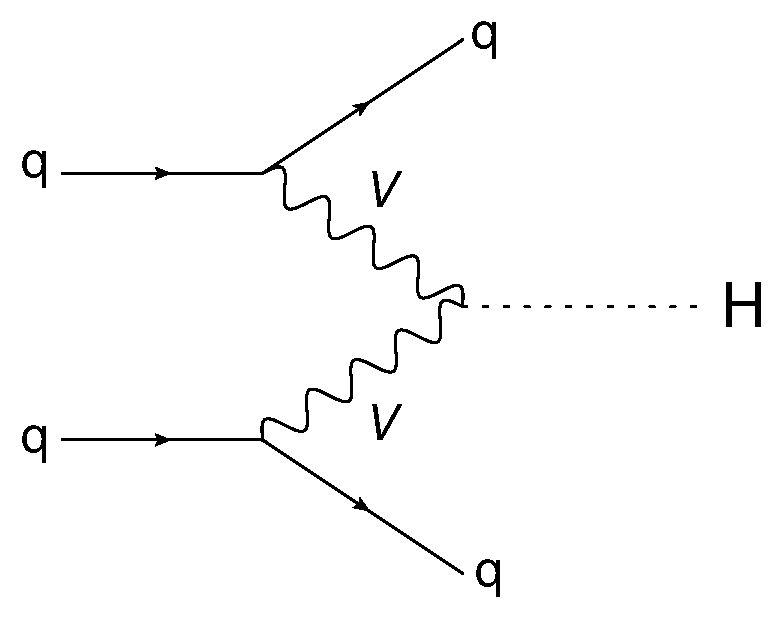
\includegraphics[width=1\linewidth]{T/FIGS/vbf}
					\end{minipage}
					\begin{minipage}[h]{0.4\linewidth}
						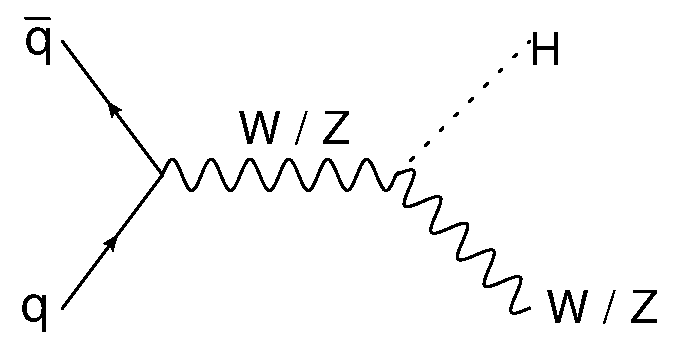
\includegraphics[width=1\linewidth]{T/FIGS/whzh}
					\end{minipage}
					\quad\quad
					\begin{minipage}[h]{0.4\linewidth}
						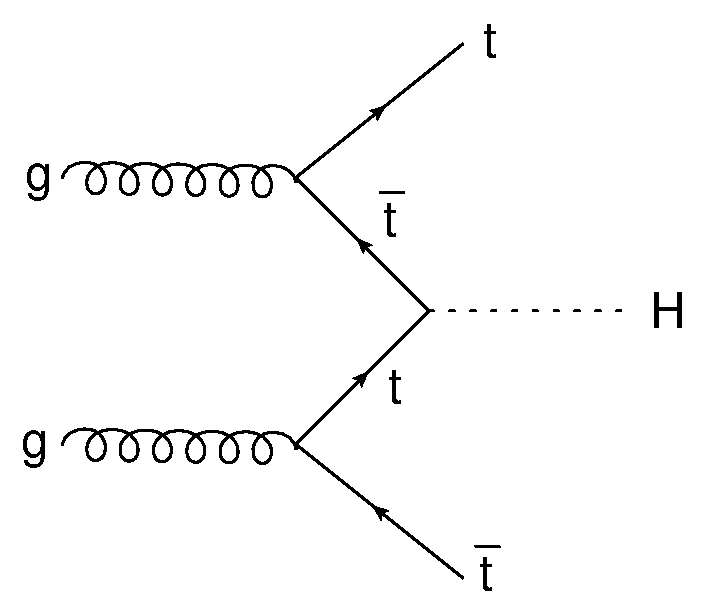
\includegraphics[width=1\linewidth]{T/FIGS/tth}
					\end{minipage}
				\caption[Feynmann diagrams of lowest order Higgs production processes]{Lowest order Feynmann diagrams for gluon-gluon fusion (\ggF), $W/Z$ associated production ($WH/ZH$) and top anti-top associated production ($t\bar{t}H$) \cite{higgsproduction}.}
				\label{fig:higgsproddiag}
			\end{figure}

			\begin{figure}[h]
				\centering
				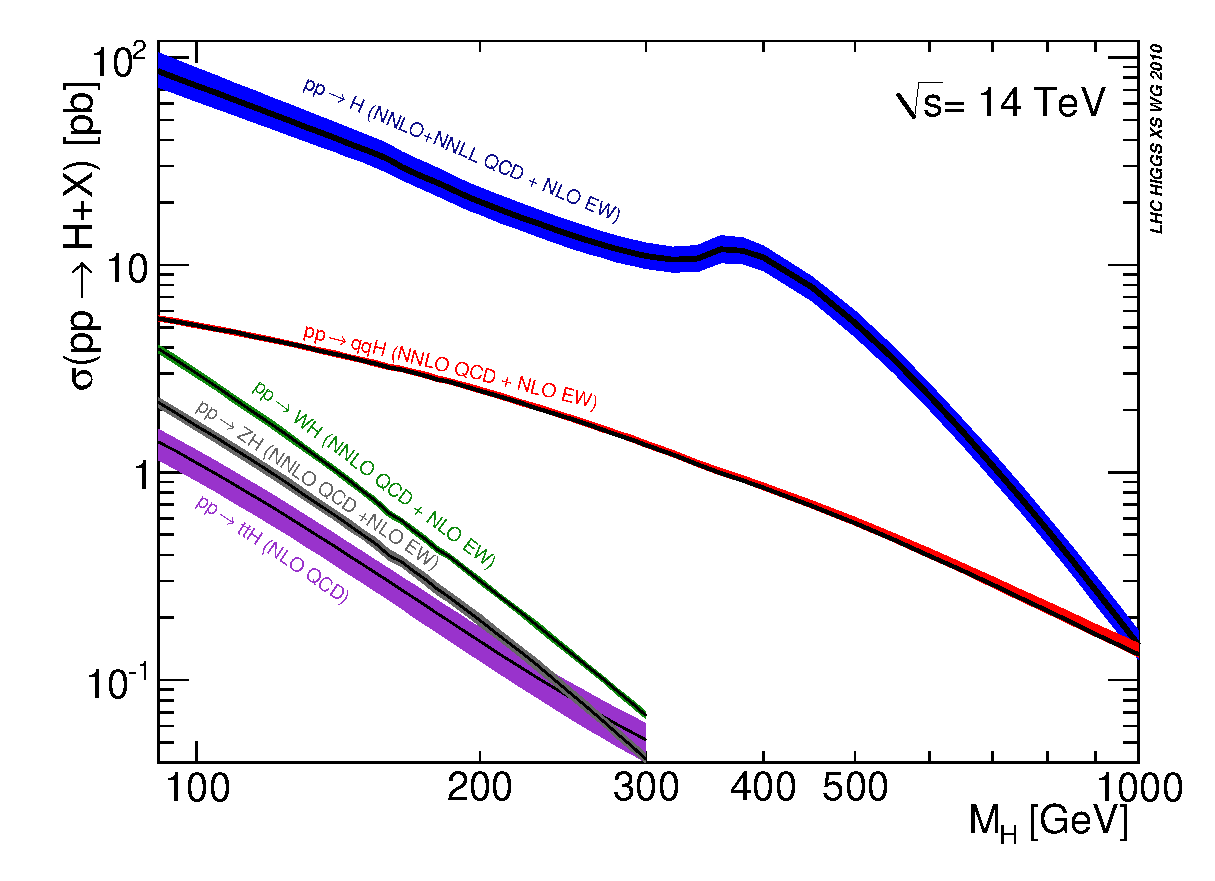
\includegraphics[width=0.7\linewidth]{T/FIGS/YRHXS_Summary_fig3}
				\caption[Higgs production cross section as a function of Higgs mass at a $\sqrt{s}=14$TeV]{SM Higgs Production cross section for $\sqrt{s}=14$ TeV. $\,pp\rightarrow H$ corresponds to gluon-gluon fusion production and $pp\rightarrow qqH$ vector boson fusion. \cite{LHCHiggsCS}}
				\label{fig:higgsproductionCS}
			\end{figure}



		The dominant production mechanism for the Higgs boson in hadron colliders is the \ggF\, production via in intermediate quark loop. The dynamics of this mechanism are controlled by strong interactions, thus calculations of QCD corrections are necessary for any accurate predictions, and have been computed up from next-to-leading order (NLO) to N$^3$LO for the \ggF\ process in recent years, along with the inclusion of Electro-Weak corrections in the cross section calculations \cite{LHCHiggsCS}.

	\subsection{Vector Boson Fusion}
	\label{t:VBF}

		Production of a Higgs boson from the fusion of vector bosons radiated from initial-state quarks is the second largest cross-section at the LHC, and is useful as a production mode due to topological characteristics which can distinguish the event from \ggF. In \VBFHBB, the characteristic topology is a pair of
		central \bjets forming the Higgs candidate, and two forward, close to the beam line VBF jets formed from remnants of the initially colliding protons as displayed in Figure \ref{fig:T:vbf}. In addition central jet activity is suppressed due to the lack of colour exchange between the colour single Higgs boson and the decay \bquarks \cite{VBF2004}.  These distinct features mean that while the cross section for VBF at a Higgs mass of $< 200$ GeV is dominated by \ggF, the easy to detect signature means the channel is a cornerstone of searches for the Higgs boson.


	\subsection{Higgs Decay}

		The branching ratios for decays of the Higgs boson in the Standard Model have been extensively determined using Monte-Carlo event generators. As is to be expected, the relative cross-sections of the decay modes are strongly dependent on the mass of the Higgs boson, as highlighted in Figure \ref{fig:higgsbrlm}.

		\begin{figure}[h]
			\centering
			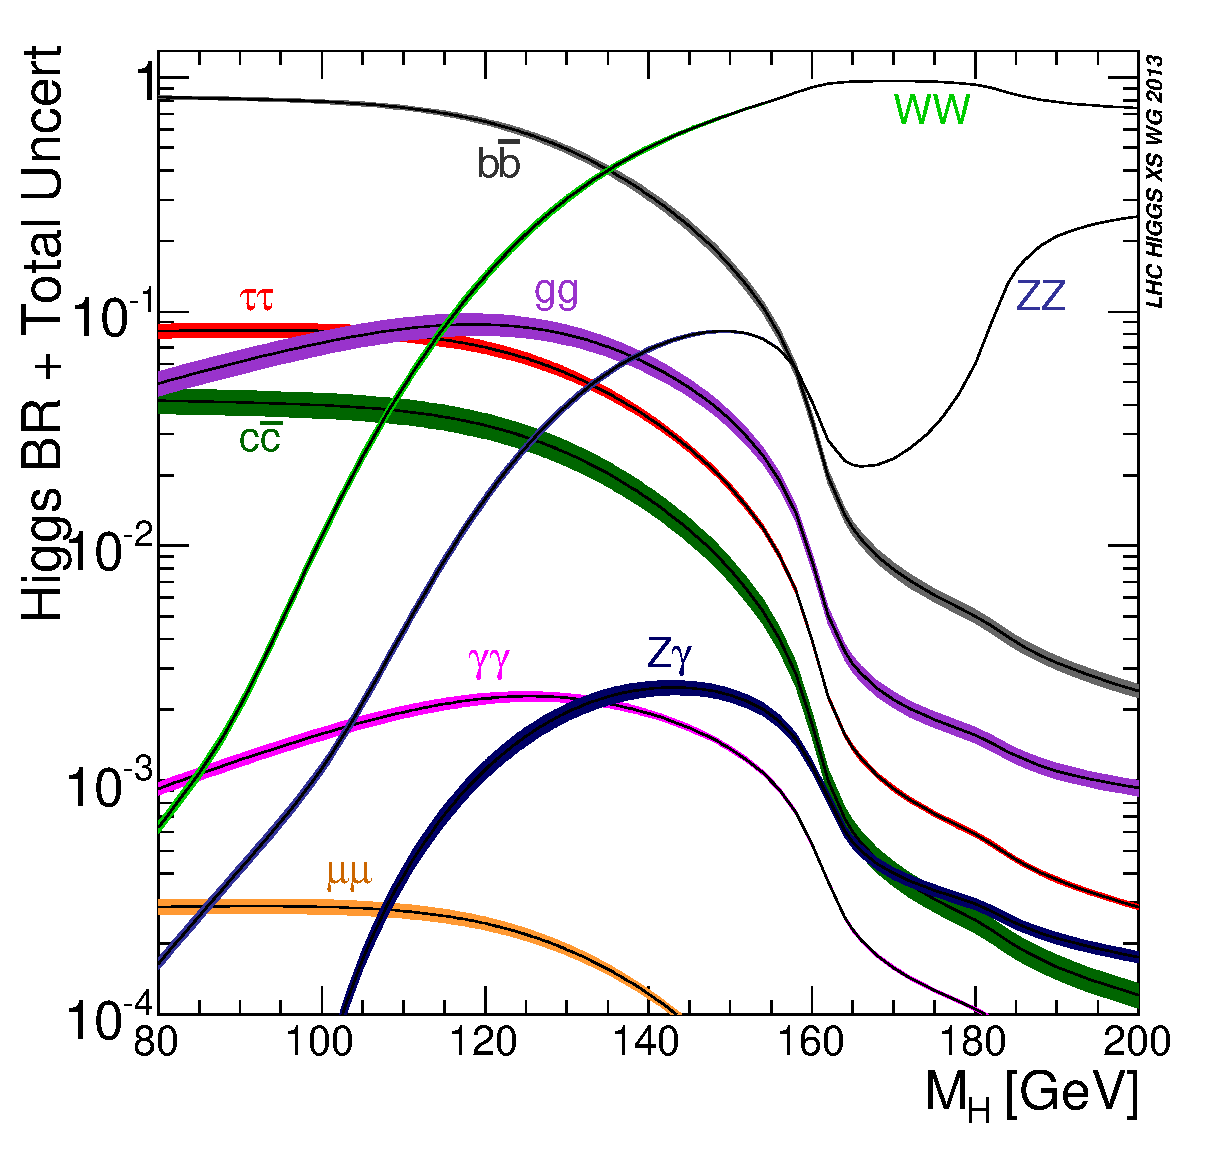
\includegraphics[width=0.5\linewidth]{T/FIGS/Higgs_BR_LM}
			\caption[Branching ratios of Higgs decay channels as a function of Higgs mass]{Higgs decay branching ratios with their uncertainties for the low mass region plotted as a function of Higgs mass \cite{LHCHiggsXS2013}.}
			\label{fig:higgsbrlm}
		\end{figure}

		\newpage
		While observations consistent with the Standard Model Higgs boson have been made for the $H\rightarrow \gamma\gamma$, $H\rightarrow ZZ$, $H\rightarrow W^+W^-$ and $H\rightarrow \tau^+\tau^-$ channels, observation of th $H\rightarrow bb$ decay channel is significantly hindered owing to the large background from multijet production in hadron collisions. Despite this, the topology of the VBF production mechanism makes it a viable option for observation of the  $b\bar{b}$ decay channel.

	\subsection{Summary of Current Higgs Measurements}

	\subsection{Searches for \VBFHBB\}

		Searches for the \VBFHBB\, interaction look for a resonance in the invariant mass of a pair of jets containing \bquarks ($m_{bb}$) in events with the characteristic topology. This characteristic topology distinguishes the signal events from the multijet events that form the dominant background with a non-resonant $m_{bb}$ spectrum. An additional resonant background contribution to the \mbb spectrum is due to decay of a $Z$ boson to two jets in association with two jets.

		In the most recent searches for the Higgs boson produced via VBF, which this analysis emulates, the \VBFHBB\, events are indistinguishable from the \ggF\, events, and are separated using a multivariate boosted decision tree (BDT) analysis to refine the phase space to the most VBF sensitive BDT regions.


\endinput


\graphicspath{{D/FIGS/}{.}}
\chapter{Detector}\label{c:Det}

\section{The Large Hadron Collider}

\section{The ATLAS Detector}

\section{Triggers}

\section{Object Reconstruction}
	
	\subsection{Jets}
	
	\subsection{\bjets}

\section{\textit{b}-Tagging}
\label{det:btagging}

	Identification of \bquark jets in ATLAS is based on combining the output of three separate \btag algorithms: Impact Parameter based (IP2D and IP3D, described in Section \ref{det:btag:ip}), Secondary Vertex based (SV, described in Section \ref{det:btag:sv}) and Decay Chain based (JetFitter, described in Section \ref{det:btag:jf})into a multivariate discriminant (MV2, covered in Section \ref{det:btag:mv}) which is used to distinguish the jet flavours. These algorithms have undergone continuous improvement over the Run-2 cycle of the LHC to improve the separation of jet flavours. 
	
	\subsubsection{IP2D and IP3D: Impact Parameter based Algorithms}
		\label{det:btag:ip}
		
		The typical topology for a \bhadron of a secondary vertex displaced from the hard scatter interaction point as a results of the lifetime of \bquark is used as the basis of these algorithms. Impact parameters of tracks from the secondary vertex are computed with respect to the primary vertex of the interaction. The IP2D algorithm uses a transverse impact parameter ($d_0$) defined as the distance of closest approach of a track to the  primary vertex in $r$-$\phi$ plane around the vertex. The IP3D algorithm uses both the transverse and a correlated longitudinal impact parameter ($z_0\sin\theta$), defined as the distance between the point of closest approach in $r$-$\phi$ and the primary vertex in the longitudinal plane. \todo{I kind of want a diagram here, but that doesn't appear to be the norm}. These parameters typically have large values as a result of the lifetime of \bquark. The signs of the impact parameters are also defined to take account of if they lie infront or behind the primary vertex with respect to the jet direction, with secondary vertices occuring behind the primary vertex normally due to background.
		
		The significance of the impact parameter values ($\frac{d_0}{\sigma_{d_0}}$, $\frac{z_0}{\sigma_{z_0\sin\theta}}$) for each track are compared to probability density functions obtained from reference histograms derived from Monte Carlo simulation, with each track being compared to a selection of reference track categories. This results in weights which are combined using a log-likelihood ratio (LLR) discriminant to compute an overall jet weight separating the $b$, $c$, and light-jet flavours from each other. \cite{btagOptimisation, bTagPerformance}
		
	\subsubsection{SV1: Secondary Vertex Finding algorithm}
	\label{det:btag:sv}
	
		The secondary vertex algorithm uses the decay products of the \bhadron to reconstruct a distinct secondary vertex. The algorithm uses all tracks that are significantly displaced from the primary vertex associated with the jet, forming vertex candidates for all pairs of track, while rejecting any vertices that would be associated with decay of long lived particles (e.g. $K_s$, $\Lambda$), photon conversions or interactions with the material in the detector. The tracks forming these vertex candidates are then iteratively combined and refined to remove outliers beyond a $\chi^2$ threshold leaving a single inclusive vertex.
		
		The properties of this secondary vertex are used to differentiate the flavour of the jet. The SV1 algorithm is based on a LLR formalism similar to the IP algorithms, and makes use ot the invariant mass of all charged tracks used to reconstruct the vertex, the number of two track vertices and the ratio of the invariant mass of the charged tracks to the invariant mass off all tracks. In addition the algorithm is signed in a similar fashion to the IP algorithms and uses the $\Delta R$ between the jet direction and secondary vertex displacement direction in the LLR calculation. The algorithm uses distributions of these variables to distinguish be      tween the jet flavours. \cite{btagOptimisation, bTagPerformance} \note{Might be worth mentioning the way these are trained}
		
	\subsubsection{JetFitter: Decay Chain Multi based Algorithm}
	\label{det:btag:jf}
	
		The JetFitter algorithm exploits the topological structure of weak \bhadron and \chadron decays inside the jet to reconstruct a full \bhadron decay chain. A Kalman filter \todo{Either understand or just cite} is used to find a common line between the on which lie the $b$, $c$ and primary vertices to approximate the \bhadron flight path. A selection of variables relating to the primary vertex and the properties of the tracks associated with the jet are used as input nodes in a neural network. This neural network uses the input variables and \pt and $|\eta|$ variables from the jets, reweighted in the kinematic variables to ensure the spectra of the kinematics are not used in the training of the neural net. The neural network outputs a discriminating variable relating to each jet flavour which are used to tag the jets. \cite{btagIdentification}
		
	\subsection{Multivariate Algorithm}
	\label{det:btag:mv}
	
	The output variables of the three basic algorithms described prior are combined as input into the Multivariate Algorithm MV2. MV2 is a Boosted Decision Tree (BDT) algorithm which has been trained on $t\bar{t}$\note{Why?} events to discriminate \bjets from light and \cjets. The algorithm makes use of the jet kinematics in addition to the tagger input variables to prevent the kinematic spectra of the training sample from being used as discriminating factor. \note{list all input variables?} The MV2 algorithm is an revised version of the MV1 algorithm used during Run-1 of the LHC, and has three sub-variants (MV2c00, MV2c10, and MV2c20) of the algorithm distinguished by the exact background composition of the training sample. The naming convention initially referred to the \cjet composition of the training sample, e.g. for MV2c20 the \bjets are designated as signal jets where a mixture of 80\% light jets and 2-\% \cjets was designated as background. 
	
	The MV2 algorithm has a set of working points, defined by a single value of the output distribution of the algorithm, which are configured to provide a specific \bjet selection efficiency on the training $t\bar{t}$ sample. Rather than being used independently, physics analyses will make use of several working points as an increase in \bjet efficiency (corresponding to \textit{looser} \bjet selection) will bring an increased mistag rate of light and \cjets.
	
	These algorithms were refined prior to the 2016 Run-2 data-taking session in response to \cjets limiting physics analyses more the light-jets. This change  to enhance the \cjet rejection meant that for the MV2c10, the \cjet fraction was set to 7\% in training and the fraction for MV2c20 was 15\%. There were a selection of other improvements to the algorithm made to the algorithm relating to the BDT training parameters and the use of the basic algorithms before the 2016 data taking. With these refinements, the MV2c10 algorithm was found to provide a comparable level of light-jet rejection to the original 2015 Mv2c20 algorithm with impoved \cjet rejection, so was chosen as the standard \btagging algorithm for 2016 analyses. \cite{btagOptimisation}
	
	
	
	
	
\endinput


\graphicspath{{ES/FIGS/}{.}}
\chapter{Event Selection}\label{c:ES}

	This chapter describes the selection criteria for data and simulated events, along with the specific calibrations and configurations used in the extraction and reconstruction of the objects making up the analysis. The event selections described here were chosen to target the typical \VBFHBB\, final state topology described in Section \ref{t:VBF}.

	\section{ATLAS Event Data}

	The raw data from the ATLAS detector is stored in a proprietary data format used by the ATLAS experiment, the Analysis Object Data (AOD) format. This is the output of the event reconstruction software, with each event having a corresponding discrete entry. For Run-2 of the LHC experiment, this was upgraded to the xAOD format, which is readable by ROOT \cite{ROOT}, a modular software framework managed by CERN and designed specifically for analysis of large datasets with complex statistical analysis, visualisation of data and storage. The xAOD format is a many leveled branching tree structure, with nodes of the tree grouping together related information from each event, and has an associated Event Data Model (EDM) to standardise classes, interfaces and types for representation of an event facilitating simple analysis \cite{xAOD}.

	Analyses typically make use of a derivation framework to refine the complete xAOD into a more selective Derived xAOD (DxAOD) which will normally only contain the relevant objects to a target analysis, and results in a smaller dataset that is much easier to manipulate, store and operate over. These derivations are produced using the ATLAS bulk data processing framework Athena \cite{athena}. The computation framework used for analysis of the xAOD data is the internally developed AnalysisBase suite of tools. The analysis presented in this dissertation uses AnalysisBase Release \texttt{2.4.31} and made use of the EventLoop package for event processing.

	This set of tools is used for both the real event data and the simulated Monte-Carlo data, with DxAODs of both datasets forming the core data for any ATLAS physics analysis. These datasets, following from the large output rate of the LHC, are extremely large, necessitating the use of parallelised computation to perform any statistically significant analysis. The computational framework developed at ATLAS is designed to perform concurrent computation, and processing, making use of the Worldwide LHC Computing Grid \cite{grid} to provide the necessary hardware capacity.

	\section{Datasets}

	The proton-proton collision data was recorded at a centre-of-mass energy of $\sqrt{s}=13$TeV in 2016. In this dissertation, Data Period D was used owing to limited storage space on analysis computing facilities. For events from the ATLAS detector to be considered usable for analysis, there are certain quality criteria that need to be passed by the event. Events are subdivided into luminosity \textit{blocks}, which are marked as \textit{good} if there are no flaws in the data integrity or missing information from the detector readout. The events were marked as \textit{clean} if there were no errors reported for the tracker or calorimeter components of the detector, and only clean events were studied.

	Information on whether certain luminosity blocks are marked as clean is contained within a configuration \textit{Good Runs List} (GRL). This analysis used the all year 25ns Good Runs List (Table \ref{t:files}, Appendix \ref{a:config}), resulting in a data luminosity of $4.6$fb$^{-1}$.

	\section{Monte-Carlo simulated events}

		 The simulated VBF sample (Table \ref{t:files}, Appendix \ref{a:config}) was produced by Monte-Carlo event generators in 2015. This sample was produced using the NLO generator \textsc{powheg}~\cite{powheg} configured using the CTEQ6L1 \cite{CTEQ} set of PDFs and interfaced with \textsc{pythia8}~\cite{pythia} tuned to AZNLO \cite{AZNLO}. The response of the ATLAS detector to the Monte-Carlo events was simulated using the \textcal{GEANT4} \cite{geant4, geant4atlas} simulation, which recreates a configurable model of the ATLAS detector, and calibrations and reconstructions were executed identically using ATLAS reconstruction code on the Monte-Carlo simulated events and the real  data.

		 To accurately compare the simulated events from the Monte-Carlo samples with the real event dataset, it is necessary to normalise the Monte-Carlo samples to the total luminosity of the dataset, based on the theoretical cross-section for the interaction. The Monte-Carlo simulation assigns a weight $w_i$ to each event simulated, which are summed to give the total number of events in the Monte-Carlo sample. Each bin of any histogram in the results produced from the simulated data is reweighted using a scaling factor $w_{MC}$, given by

		 \begin{equation}
		 w_{MC} = \frac{\sigma k L}{N},
		 \end{equation}

		 where $\sigma$ is the theoretical cross section, $L$ the integrated luminosity of the real dataset, $N$ the total number of simulated events ($\Sigma_N w_i$) and $k$ the Real $K$-Factor, which is a correction to the leading order cross section to reproduce the higher order calculation for the interaction. This reweighting of the Monte-Carlo datasets allows valid comparison of the Monte-Carlo simulated events with varying data sample sizes, as in the case of the reduced data luminosity in this analysis.


	\section{Jet Extraction}
	\label{es:jetextract}

		The analysis is based on the jet objects from the detector contained in the DxAOD, the reconstruction of which is covered in Section \ref{d:jetreco}. Both the offline jet objects and the online equivalents are retrieved, but the method by which the full collection of jets is assembled differs in each case. For offline jet objects, the DxAOD contains a complete set of jets for each reconstruction algorithm, which are each associated with the relevant jet \btag\, information. Offline jets were calibrated in line with the 20.7 recommendations (Table \ref{t:config}). In addition, recorded individual jets were required to have \pt$>45$GeV.

		Recovering the trigger-level jet objects from the xAOD is done by assembling distinct object collections from the data into a single jet collection. The jets that satisfied the trigger requirements (Section \ref{es:as}) are stored as \textit{split}-jets in the data. These \textit{split}-jet objects are those that will have \btag\ decisions associated with them. Any duplicate \textit{split}-jets in this collection, determined by pairing jets and removing those with $\Delta R$ spacings below a threshold value of 0.3, are removed and the \btag\, information stored in a separate xAOD container is associated with the \textit{split}-jets. Following this all HLT trigger jets are retrieved. These HLT trigger jets are different from the \textit{split}-jets and do not possess \btag\, information. The full set of HLT jets is compared to the \textit{split}-jets and any duplicates are removed from the HLT jet collection (again using $\Delta R$ matching) to form the \textit{nonsplit}-jets. The combination of the \textit{split}-jets and \textit{nonsplit}-jets forms the complete jet collection for the trigger level event.

		This complete collection of \textit{split} and \textit{nonsplit}-jets was taken as the comprehensive full set of jets for an event. The lack of associated \btag\ information for the \textit{nonsplit}-jets meant only jets from the \textit{split}-jet list could be designated as \bjets.

		\subsection{\bjets}

		The details of \bjet\ identification are covered in Section \ref{det:btagging}. Offline $b$-jets were tagged using the MV2c10-tagger configured using the January 2017 recommendations (Table \ref{t:config}) with two defined efficiency working points: \textit{tight}, with an overall efficiency of 70\% and \textit{loose} with 85\% tagging efficiency. Online $b$-jets were tagged using the MV2c20
		-tagger as configured during the data taking, which made use of the March 2016 Recommendations (Table \ref{t:config}) with two identically defined \textit{tight} and \textit{loose} working points. The use of the older \btagging\ algorithm in the decision for the online jets was forced. The online trigger objects in the DxAOD only contain the results of the evaluated \btag, the quantities used during the calculation were previously discarded. As such, this analysis was required to use the MV2c20 algorithm for HLT jets.


	\section{\VBFHBB\, Analysis Strategy}


	\label{es:as}
		Candidate \VBFHBB\, events are selected by requiring two \textit{central} \bjets\, which form the Higgs boson candidate and two high \pt VBF-tagging jets. The analysis presented in this dissertation follows the selection criteria outlined in the 2016 Search for \VBFHBB\ at ATLAS \cite{VBFHbb8tev}. Searches using \VBFHBB\, consider two exclusive analysis channels of interesting events: the \textit{four-central} channel, which requires all four jets to be contained within the central region $|\eta| < 2.8$, and the \textit{two-central} channel which requires two jets in the central region and at least one forward jet.
		The analysis presented in this dissertation focuses on the \textit{two-central} channel as this is a more standard VBF topology.

		For the \textit{two-central} channel, the event was required to pass the \texttt{HLT\_j80\_bmv2c2070\_split\_\-j60\_bmv2c2085\_split\_j45\_320eta490} trigger. This trigger requires a single L1 jet ROI of $E_\text{T} > 40$GeV and $|\eta| < 2.5$, a second central jet ROI with $E_\text{T} > 25$, and a forward jet ROI with $E_\text{T} > 20$GeV and $3.1 < |\eta| < 4.9$.
		At the HLT, one central jet \btagged\, at the \textit{tight} working point with \pt $>80$GeV, and a jet with \pt$>60$GeV tagged at the \textit{loose} working point were both required. Finally a HLT forward jet with $E_\text{T}>45$ between $3.2 < |\eta| < 4.9$ was needed.

		Once the trigger was passed, the event was required to contain one jet with \pt$>95$GeV which was \btagged\, at the \textit{tight} working point and one additional jet with \pt$>70$GeV that passed the \textit{loose} \btag\, working point. One forward jet with $3.2 < |\eta| < 4.4$ and $p_{\text{T}}>60$GeV was required along with a final VBF jet with \pt$>20$GeV and $|\eta| < 4.4$. Finally the \pt of the $b\bar{b}$ pair was required to exceed 160 GeV. This cut is to remove kinematic sculpting of the $M_{bb}$ distribution, which for absent or lower \ptbb cuts has a pronounced bump in the $200$-$300$GeV $M_{bb}$ region. This bump is a result of the correlation between \mbb and \ptbb values. By requiring the \ptbb cut, the \mbb distribution forms a regular falling distribution. The cuts as applied in the analysis code are summarised in Table \ref{tab:cuts}

		\begin{table}[h]
		\caption[\textit{Two-central} channel event cuts]{Cutflow for the \textit{two-central} \VBFHBB\ channel.}
		\label{tab:cuts}
		\medskip
		\centering
		\begin{tabularx}{\textwidth}{p{2.5cm} X}\toprule
			Cut & Description \\\midrule
			Good Runs List & Event required to pass GRL.\\
			Clean Events & Event required to be unaffected by detector issues.\\
			Trigger & Event required to have passed the \texttt{HLT\_j80\_bmv2c2070\_split\_\-j60\_bmv2c2085\_split\_j45\_320eta490} trigger.\\
			$\geq2$ \textit{loose} & Event was required to contain at least two \bjets\ with \pt$>70$GeV tagged at the \textit{loose} working point.\\
			$\geq2$ light-jets & Event was required to contain at least two non-\bjets\ with \pt$>20$GeV.\\
			\textit{Tight} \bjet & Event was required to contain one \bjet\ with \pt$>95$GeV tagged at the \textit{tight} working point.\\
			Forward jet requirement & Event was required to contain one non-\bjet\ with \pt$>60$GeV and $3.2 < |\eta| < 4.4$.\\
			\ptbb$>160$GeV & The chosen $b\bar{b}$ pair was required to have a combined \pt$>160$GeV \\
			\bottomrule
		\end{tabularx}
	\end{table}

		The events were required to be clean events, unaffected by any small detector issues, and the jets were assigned to components of the \VBFHBB\, event as described in the following procedure. All pairs of jets that passed the \textit{loose} working point (where either of the jet pair passed the \textit{tight} working point) were considered; the pair with the highest \ptbb was selected as the Higgs candidate. An identical iterative procedure was carried out to assign the VBF pair, using jets not marked for consideration as the Higgs boson candidate. One of the VBF jet pair was required to satisfy the forward jet selection criterion, and the highest invariant mass pair was selected.

		These conditions were identical for both the Monte-Carlo simulation and data, with the exception of the trigger requirements which were not required for the simulated samples.

		In a full ATLAS analysis\cite{VBFHbb8tev}, the signal is extracted from the selected events using a Boosted Decision Tree (BDT) trained to extract the \VBFHBB\, events over non-Higgs backgrounds. Time constraints in this analysis prohibited a full BDT analysis, but discussion of boosted decision trees and training is covered in Appendix \ref{a:bdt}.


\endinput


\graphicspath{{ObP/FIGS/}{.}}
\chapter{Object Performance}\label{c:OP}

Prior to conducting a full study of TLA on the \VBFHBB\, channel, the features of jet objects reconstructed offline and within the HLT were compared to identify any performance differences in the base components of event reconstruction. The jet objects were compared on a one to one basis, by matching an online jet to an offline jet by requiring the $\Delta R$ (Section \ref{t:geometry}) value between the two jets to be below a threshold value of \DELTARTHRESHOLD. This cut was determined from a plot of $\Delta R$ values between all pairs of jets, shown in Figure \ref{f:deltaR}.

\begin{figure}[h]
	\centering
	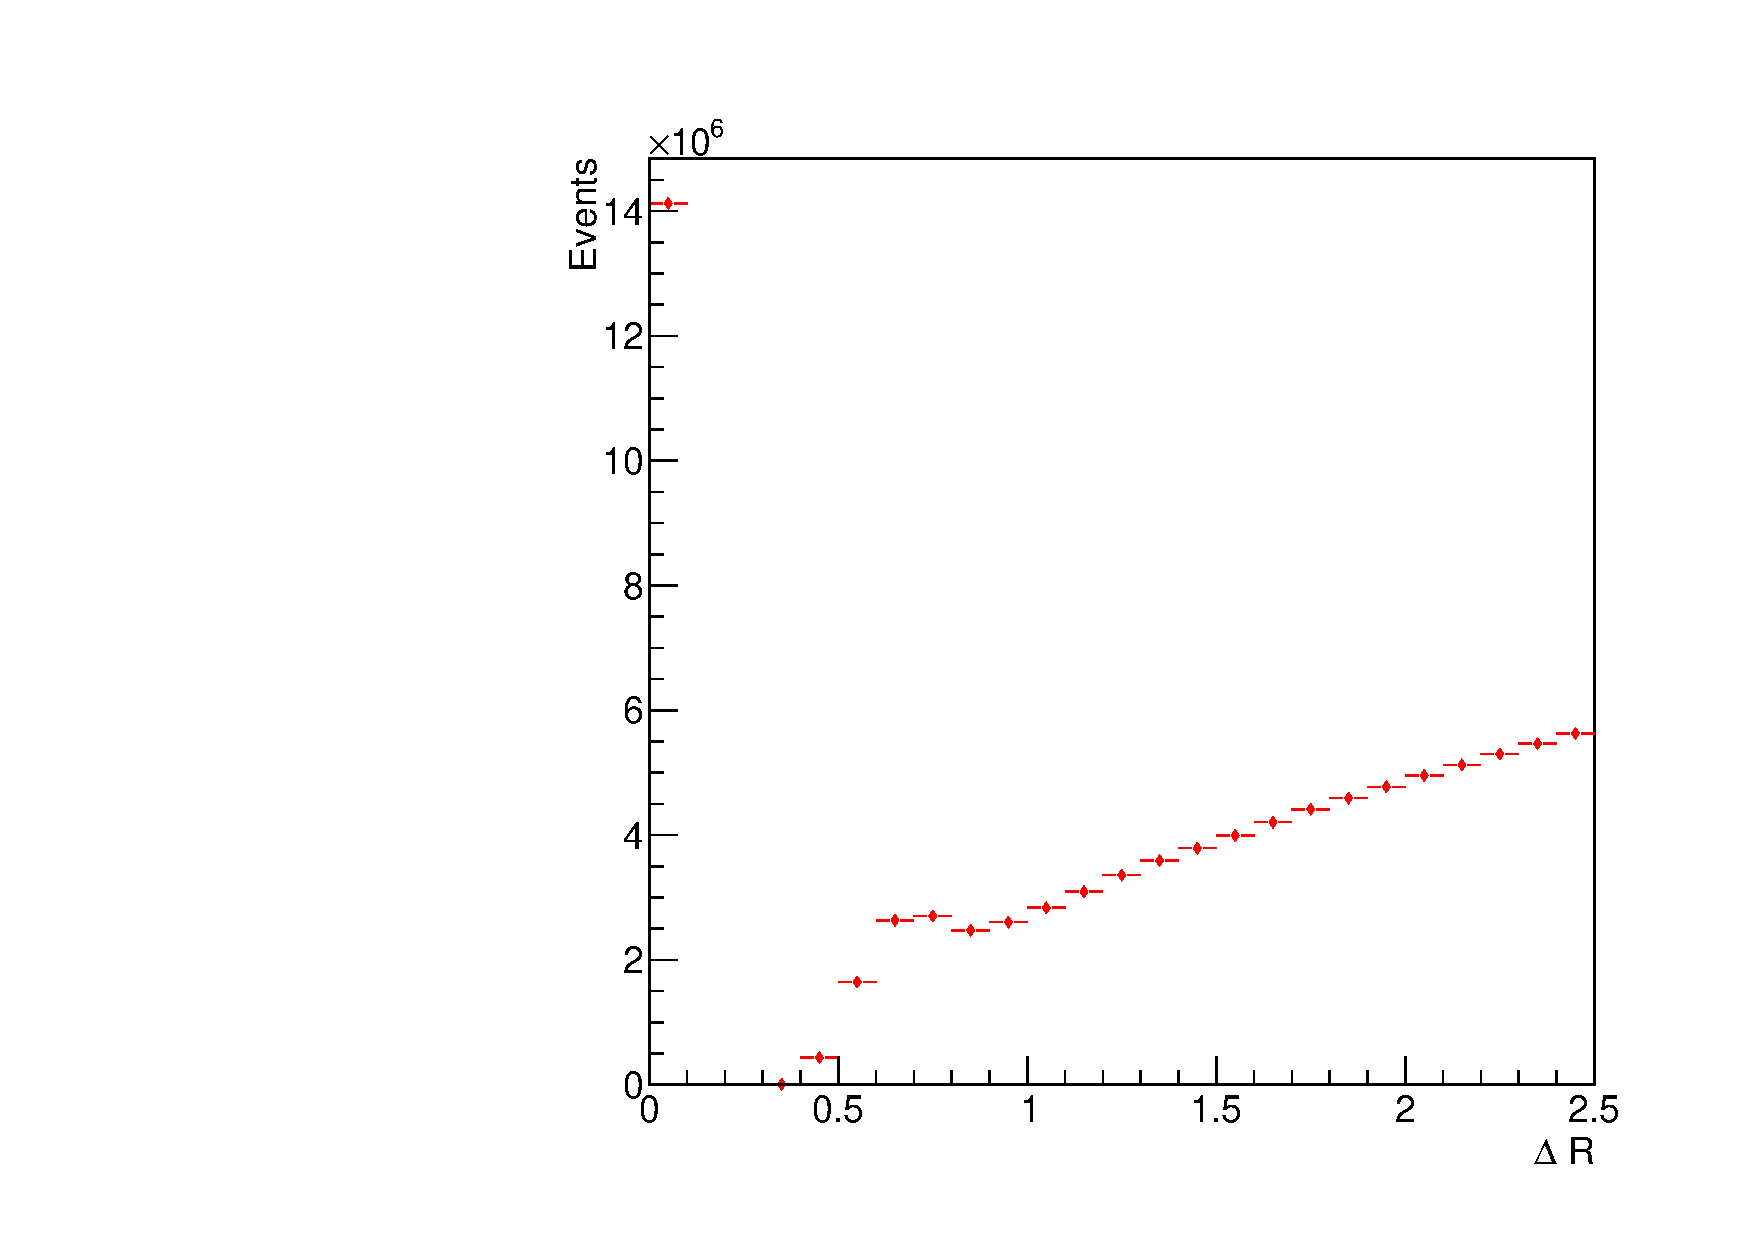
\includegraphics[width=0.5\linewidth]{deltaR}
	\caption{Plot of $\Delta R$ values for all online/offline jet pairs taken from the Monte-Carlo data. The large spike at $\sim0$ accounts for matching jets, with the higher $\Delta R$ Values corresponding to differing jet pairs.}
	\label{f:deltaR}
\end{figure}
To compare the online and offline jets, the ratio of the difference in value for (significant) jet properties between the matched jets were evaluated. These values were calculated for jet feature $X$ using:

	\begin{equation}
	\frac{\Delta X}{X} = \frac{X_{Offline} - X_{Online}}{X_{Offline}}
	\end{equation}

	where $X_{Offline}$ is the value of the feature on the offline jet, and $X_{Online}$ is from the HLT jet. Specific categories of jets within the event were compared to ensure the most relevant jets for the \VBFHBB\, analysis were comparable.

	The performance of the online and offline jet features was tested bearing in mind the final state products of the \VBFHBB\, interaction, while considering the rapidity of the produced jets. The jets used to produce these plots were taken from all analysed Monte-Carlo events  and all real data events where the trigger was passed, but the additional \VBFHBB\, requirements mentioned in Section \ref{es:as} were not enforced. In addition, given the \pt requirements of the desired event are high, only jets with \pt$>45$GeV were considered for analysis.

\section{Leading \textit{b}-jets}
\label{OP:leadingb}

	The leading \pt offline $b$-jet was selected from an event, requiring the jet to pass the \textit{Tight} \btagging working point. This jet was matched to a corresponding online jet using $\Delta R$ matching, and the properties of each of these jets compared in both Data and Monte-Carlo.

		\begin{figure}[h]
			\centering
			\begin{minipage}[h]{0.48\linewidth}
				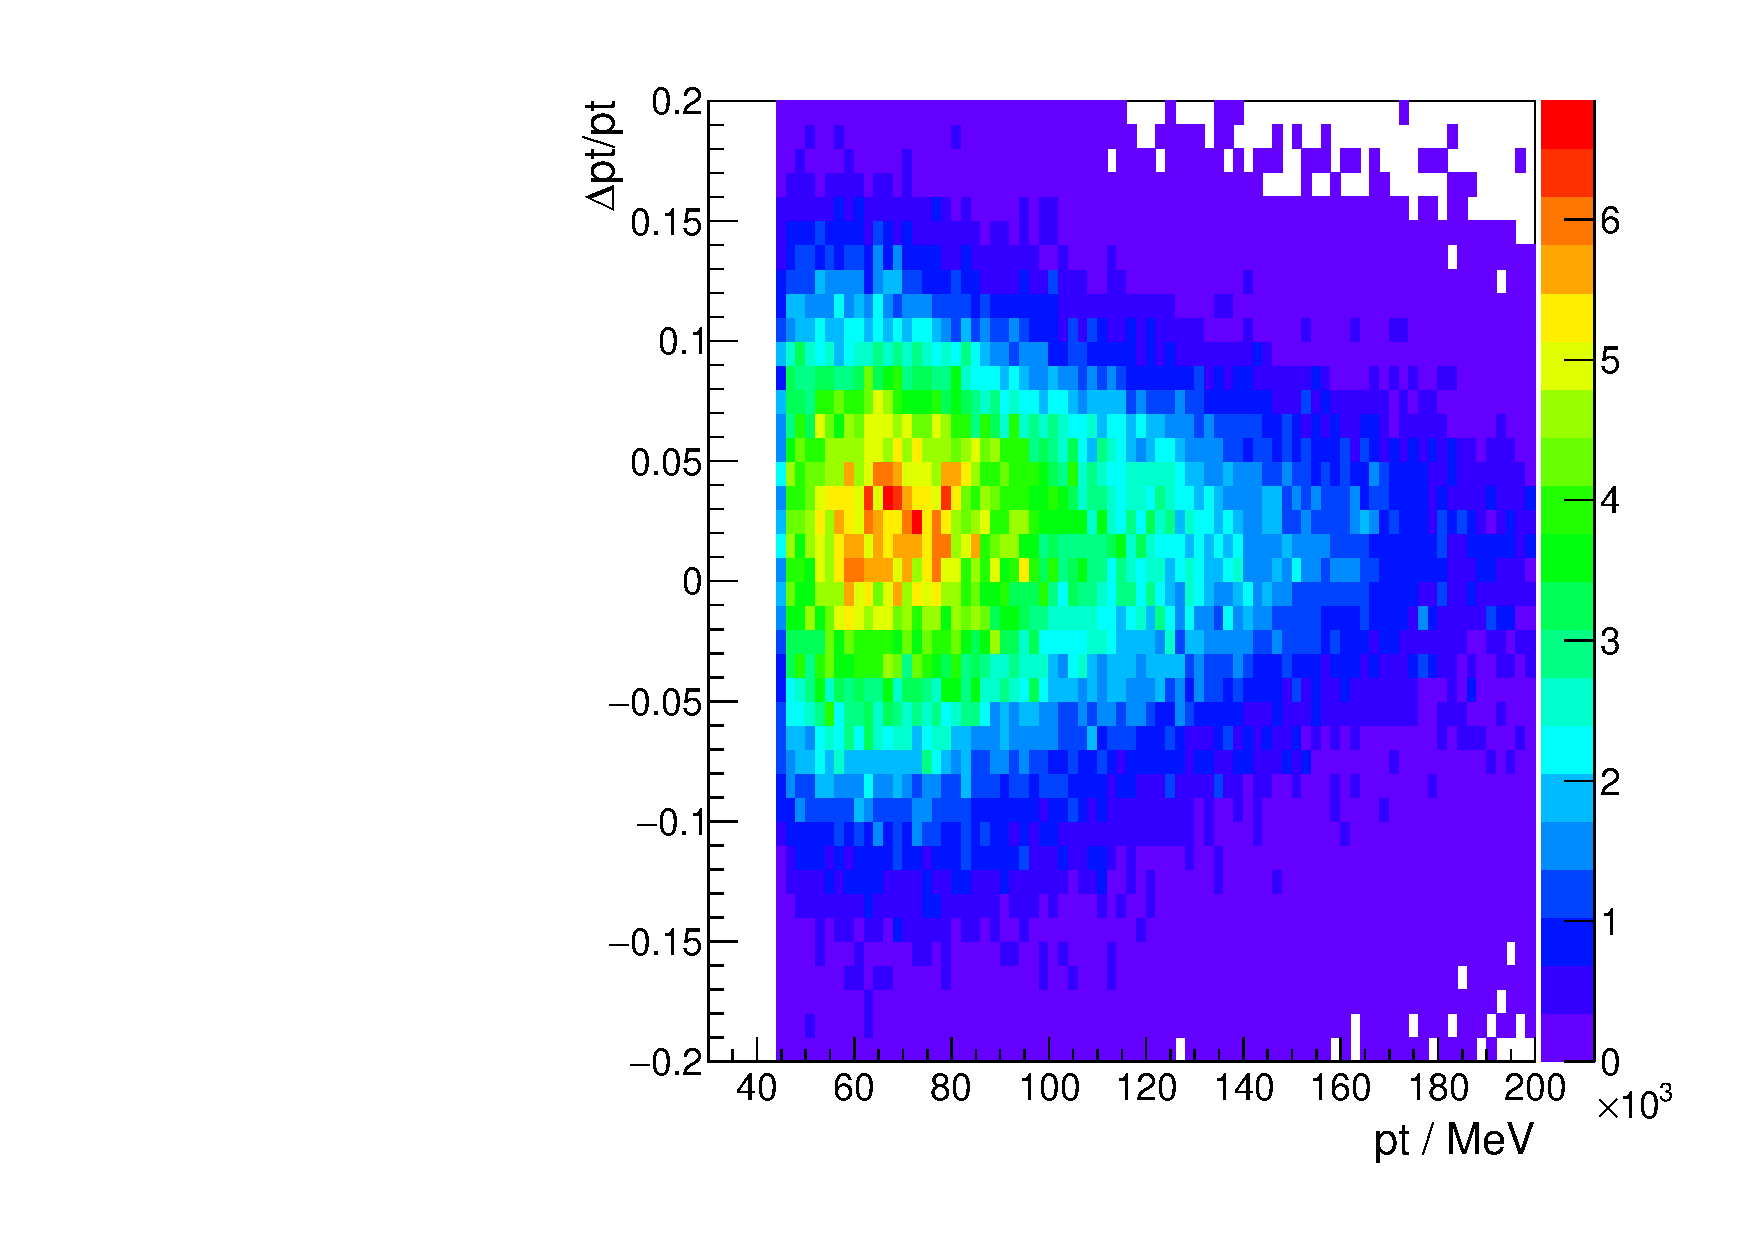
\includegraphics[width=1\linewidth]{ptRatio_Leading_BJet}

			\end{minipage}
			\quad
			\begin{minipage}[h]{0.48\linewidth}
				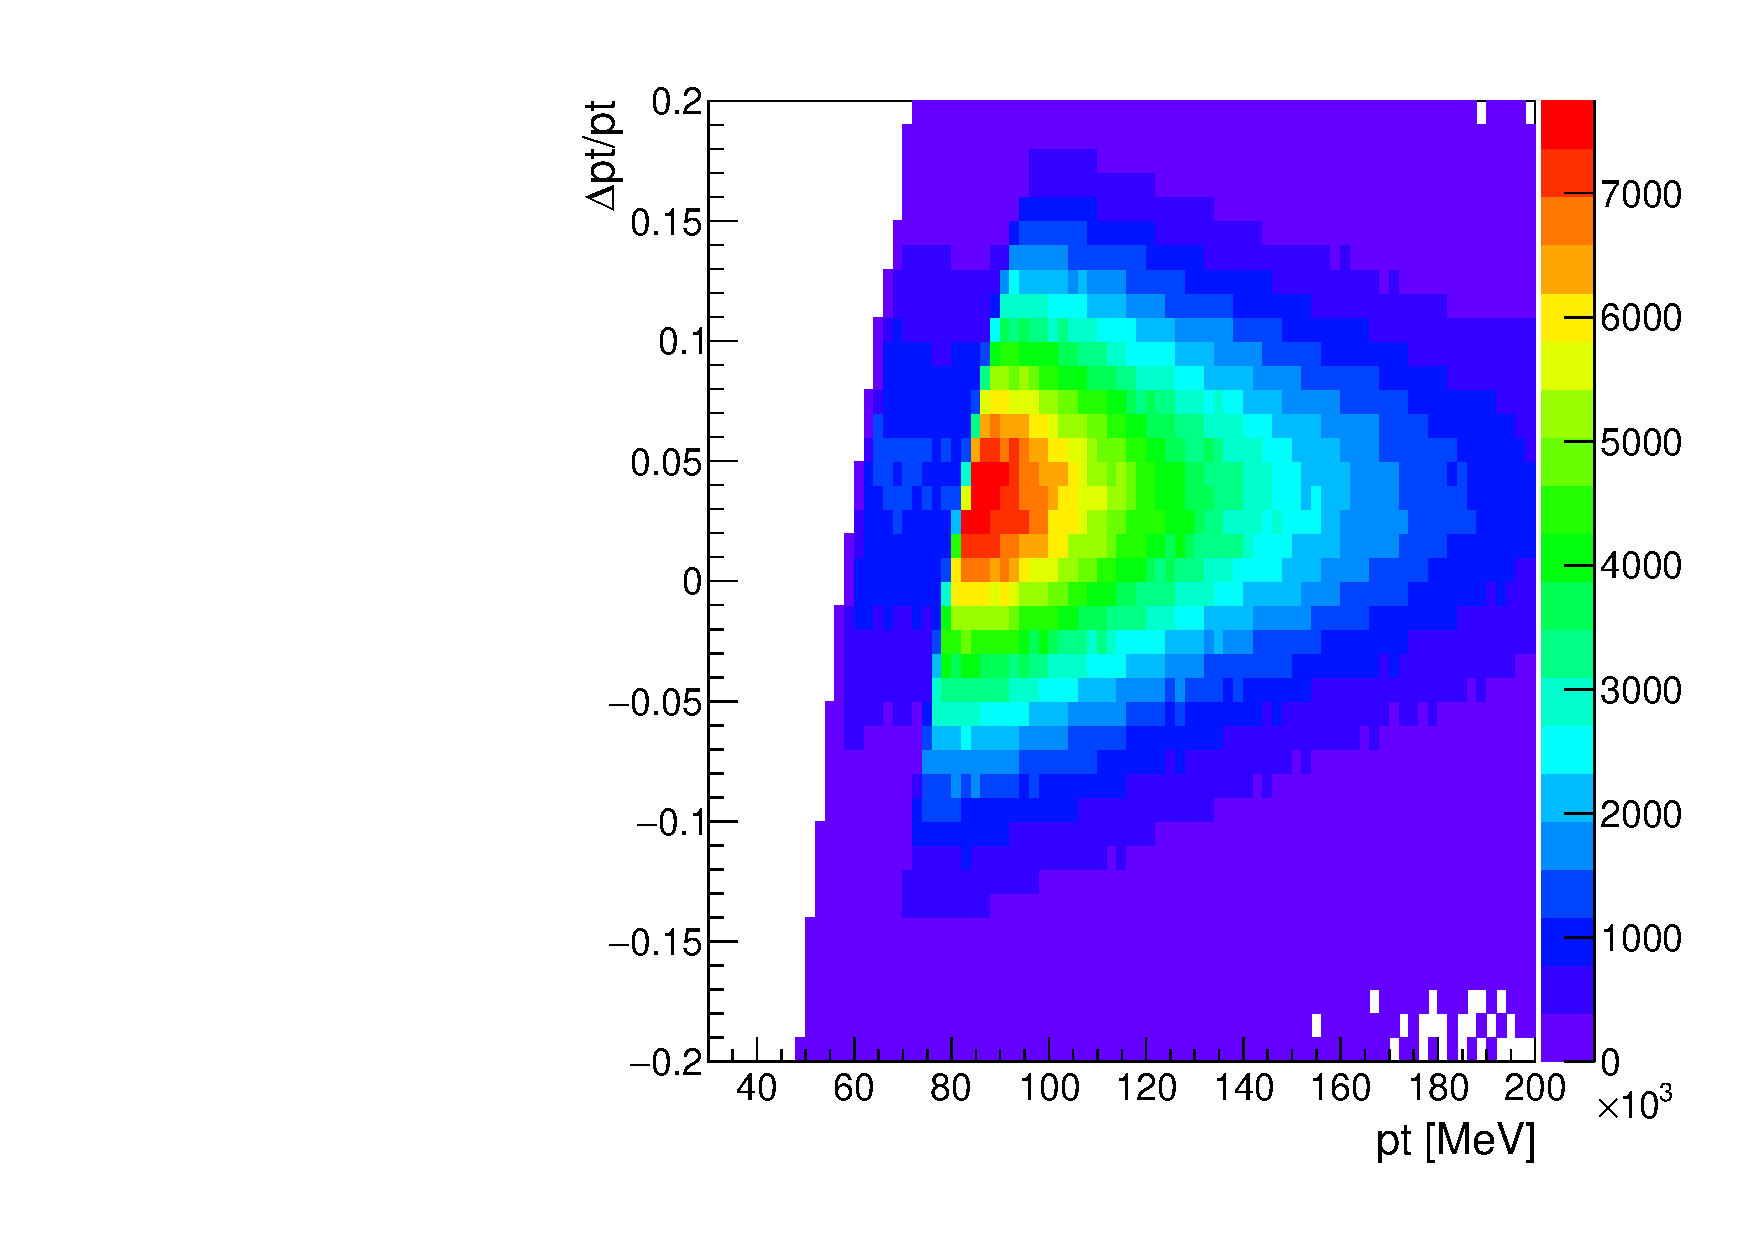
\includegraphics[width=1\linewidth]{Offline_2C_ptRatio_Leading_BJet}
			\end{minipage}
			\caption{$\Delta $\pt$_{ratio}$ for the leading \pt $b$-jet against \pt of the offline $b$-jet, plotted for Monte-Carlo simulated results (left) and real data (right).}
			\label{fig:O:leadingbpt}
		\end{figure}

		\newpage
		The comparative performance of the online and offline jets is \pt is broadly similar for events in both Data and Monte-Carlo. The bulk of the results occur with a \dptpt$\sim0$ and the two plots show a comparable drop off in \pt distribution. The distinctive curve present in the real data is the result of the trigger (Section \ref{es:as}} being applied to each event, which was not applied in the Monte-Carlo data. The real data was required to contain at least one jet with a \pt$>80$GeV which results in the steep drop-off below this cut value.

		The distribution of the \dptpt about 0 can be shown by taking a slice across the distribution for a representative \pt value. The \dptpt values were also split into $\eta$ bands to study performance at different points in the detector. For the leading \bjet, this is constrained to be within the region of the detector where \btagg\, is available.

		\begin{figure}[h]
			\centering

			\begin{minipage}[h]{0.48\linewidth}
				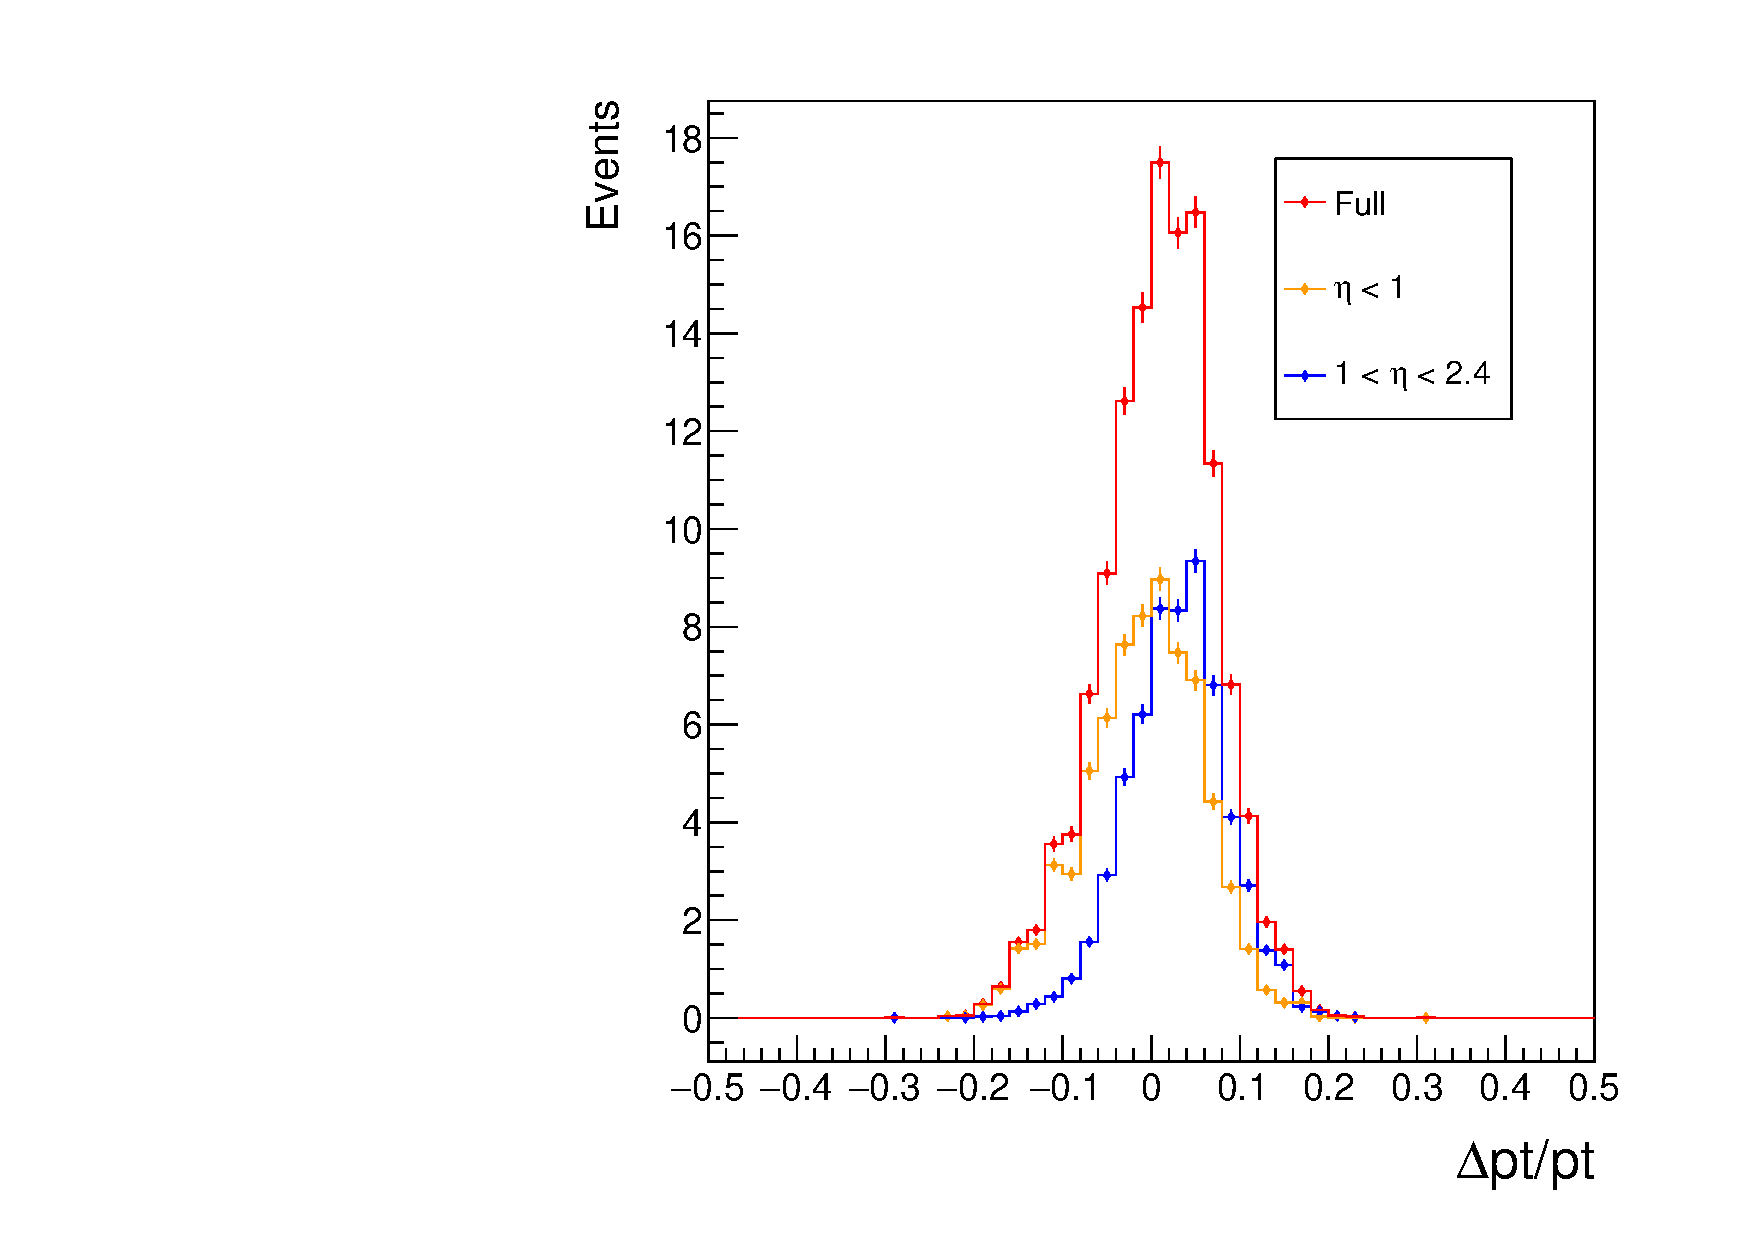
\includegraphics[width=1\linewidth]{Slices_ptRatio_Leading_BJet}
			\end{minipage}
			\quad
			\begin{minipage}[h]{0.48\linewidth}
				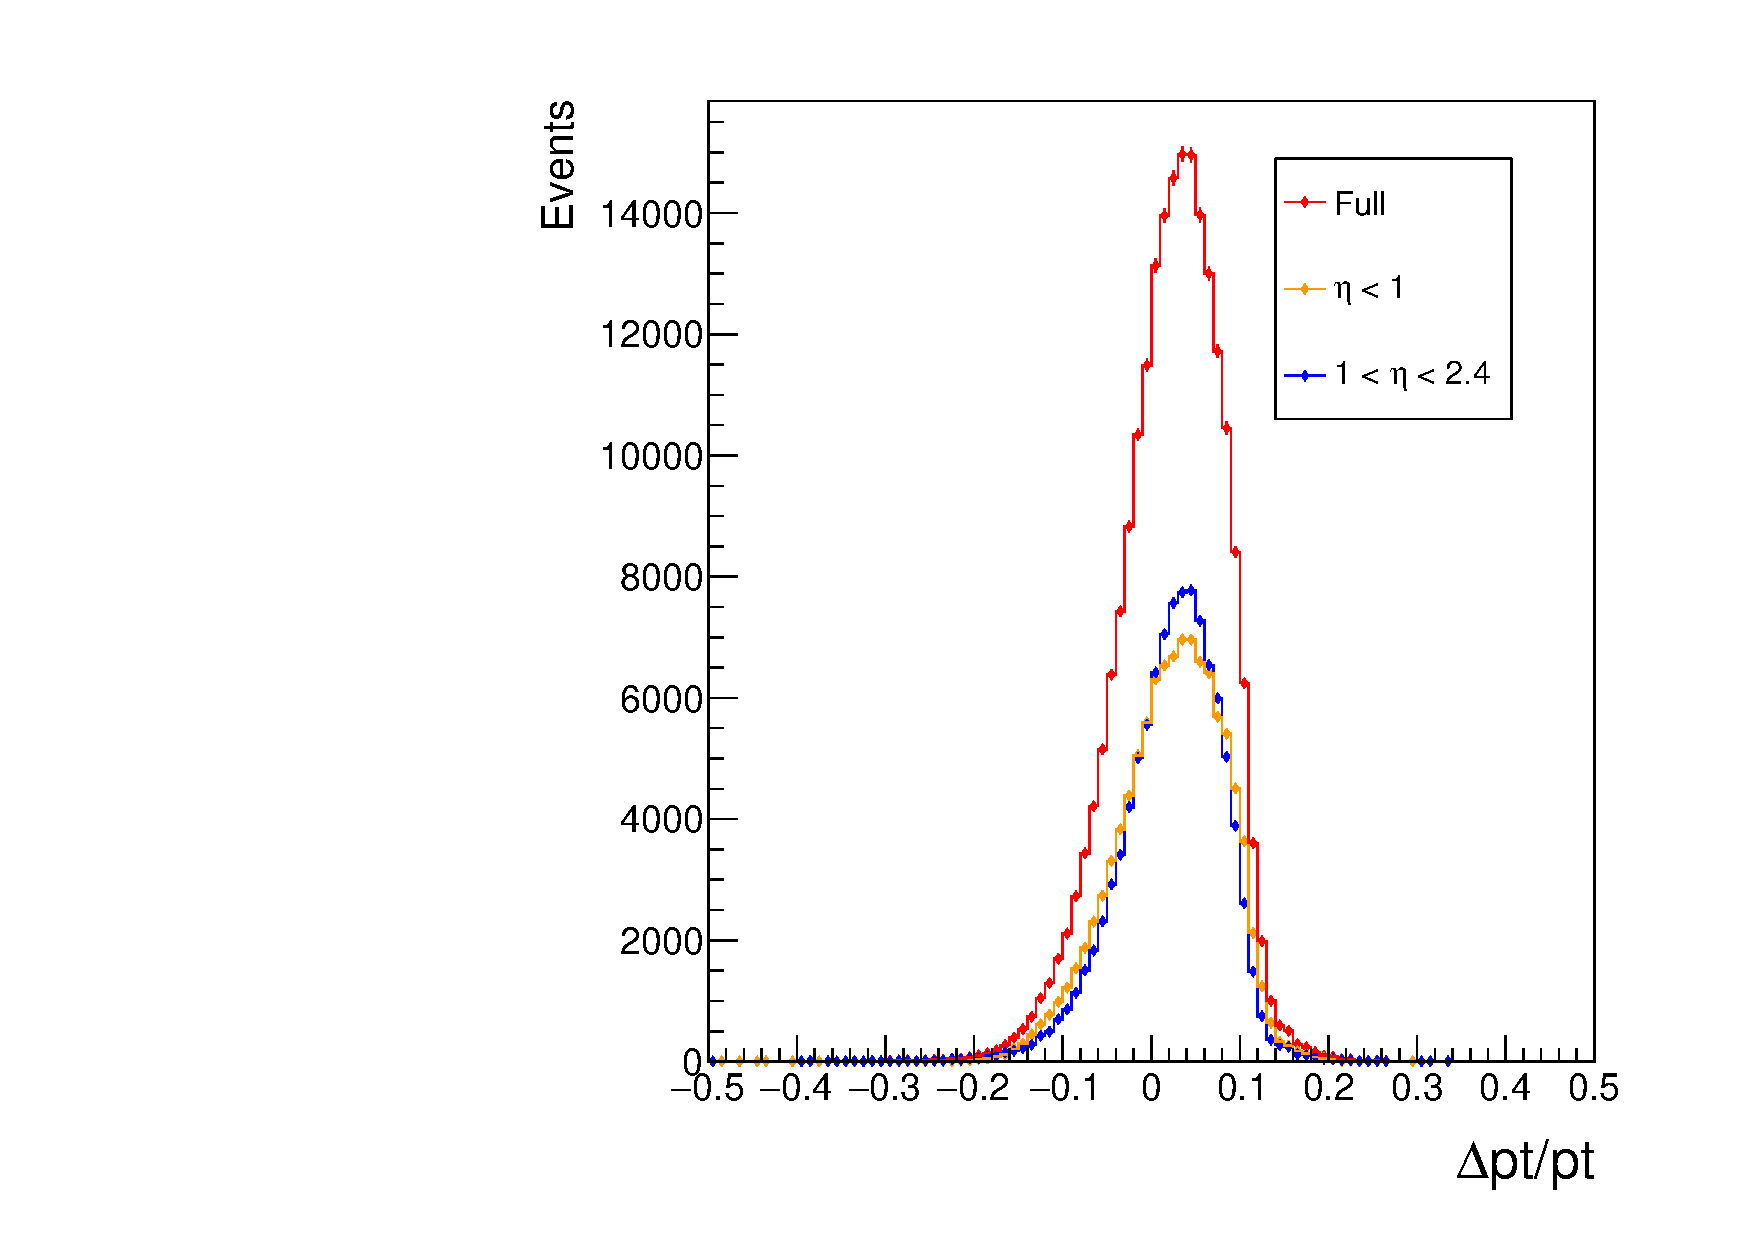
\includegraphics[width=1\linewidth]{Slices_Data_ptRatio_Leading_BJet}
			\end{minipage}
			\caption{\dptpt distribution for the leading \bjet with $89<$\pt$<91$ GeV. The distributions for all events and events split by $\eta$ region are shown. Monte-Carlo results are shown on the left and real data on the right.}
			\label{fig:O:leadingbptslice}
		\end{figure}

		 The results show similar profiles between the Monte-Carlo and Data events for \dptpt. Both plots show the offline \pt values to be consistently higher than the online, with a median shift of $4\%$ in Data and $2\%$ in Monte-Carlo. The performance between $\eta$ ranges was also consistent. The profiles broadly match the full shape of each other, but the Monte-Carlo showed a slight difference in \dptpt value as the central $\eta$ range peaked at $\sim0$. The breadth of these distributions is quite large, with both Data and Monte-Carlo showing $\pm10\%$ in \dptpt.
		 \newpage
		These comparisons can be carried out for other jet properties ($\eta$, $\phi$) to confirm the offline and online jets are behaving in a similar fashion.

		\begin{figure}[h]
			\centering
			\begin{minipage}[h]{0.48\linewidth}
				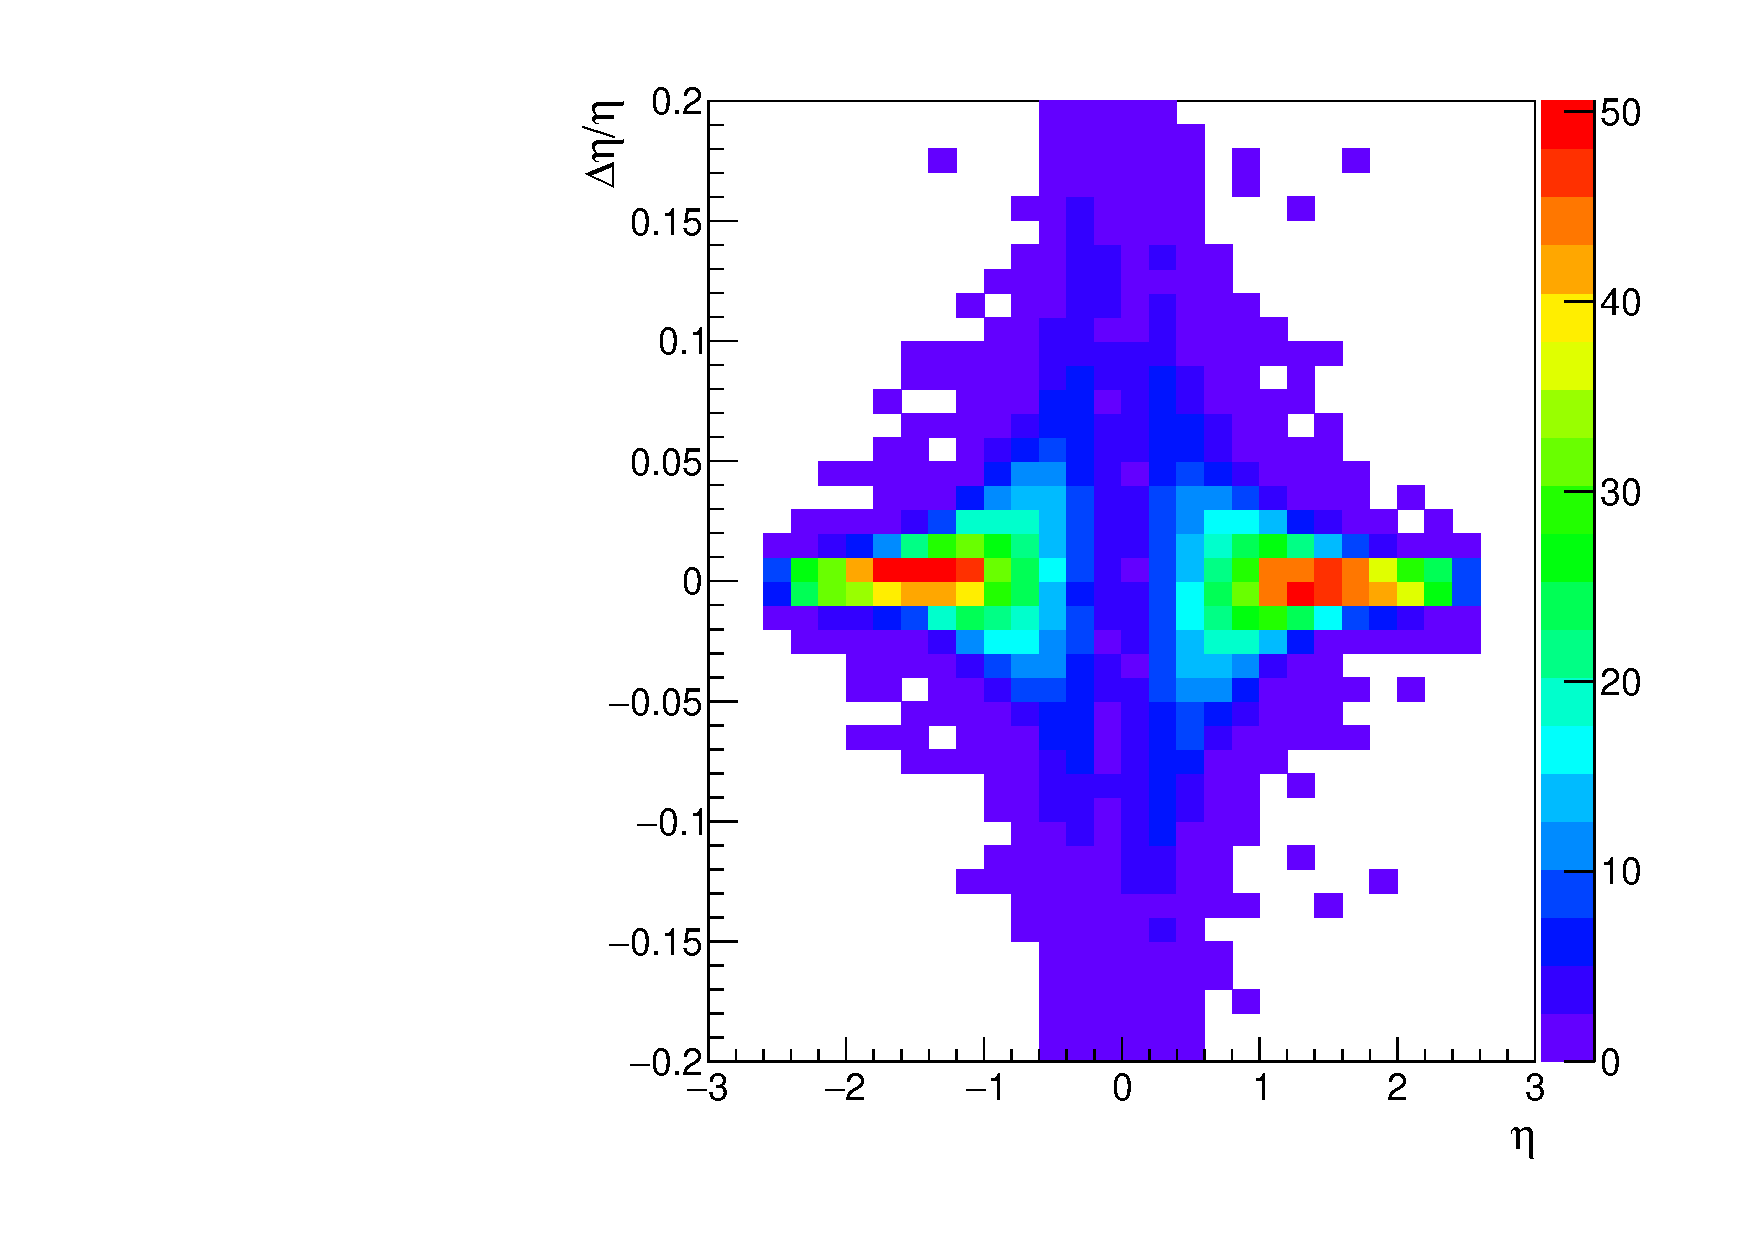
\includegraphics[width=1\linewidth]{etaRatio_Leading_BJet}

			\end{minipage}
			\quad
			\begin{minipage}[h]{0.48\linewidth}
				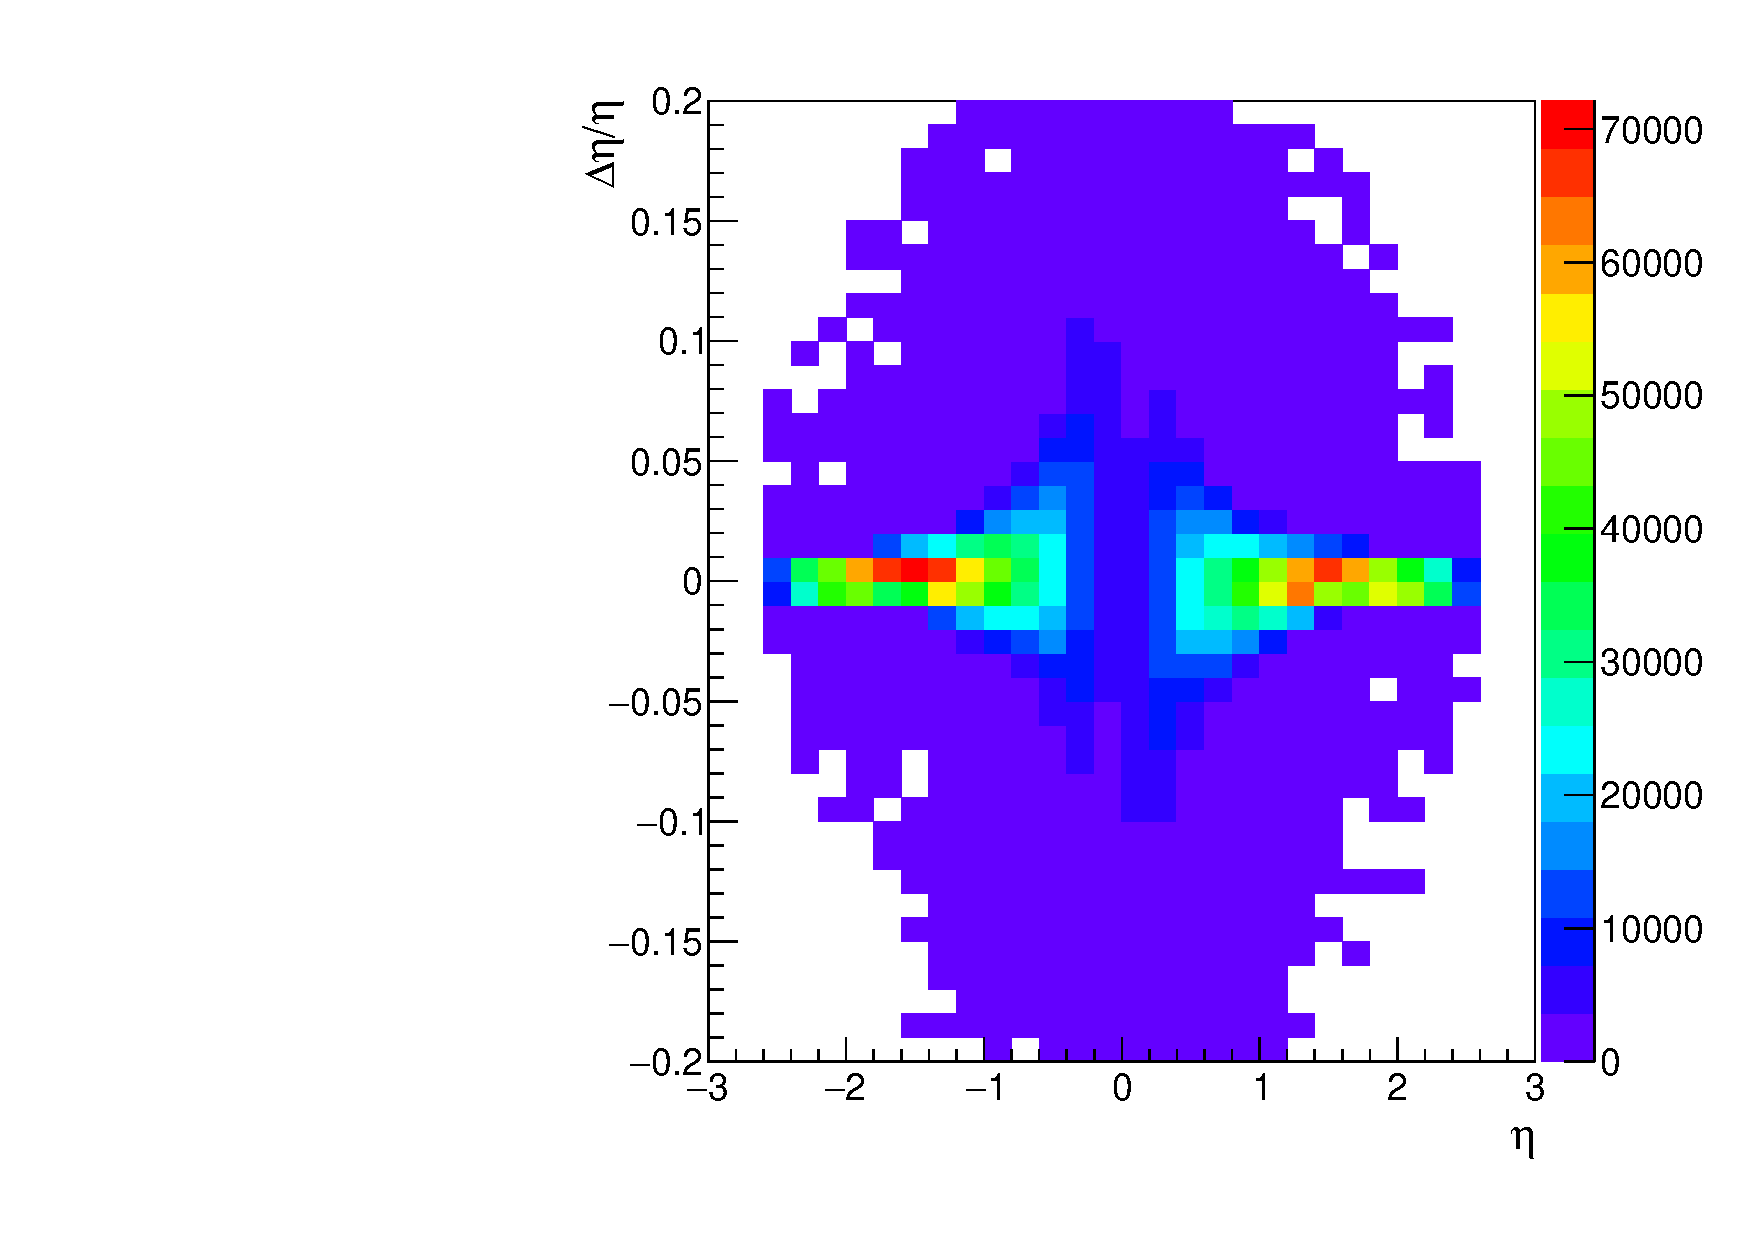
\includegraphics[width=1\linewidth]{Offline_2C_etaRatio_Leading_BJet}
			\end{minipage}
			\caption{\dee for the leading \bjet, for Monte-Carlo events (left) and real data (right).}
			\label{fig:O:leadingbeta}
		\end{figure}

		\begin{figure}[h]
			\centering
			\begin{minipage}[h]{0.48\linewidth}
				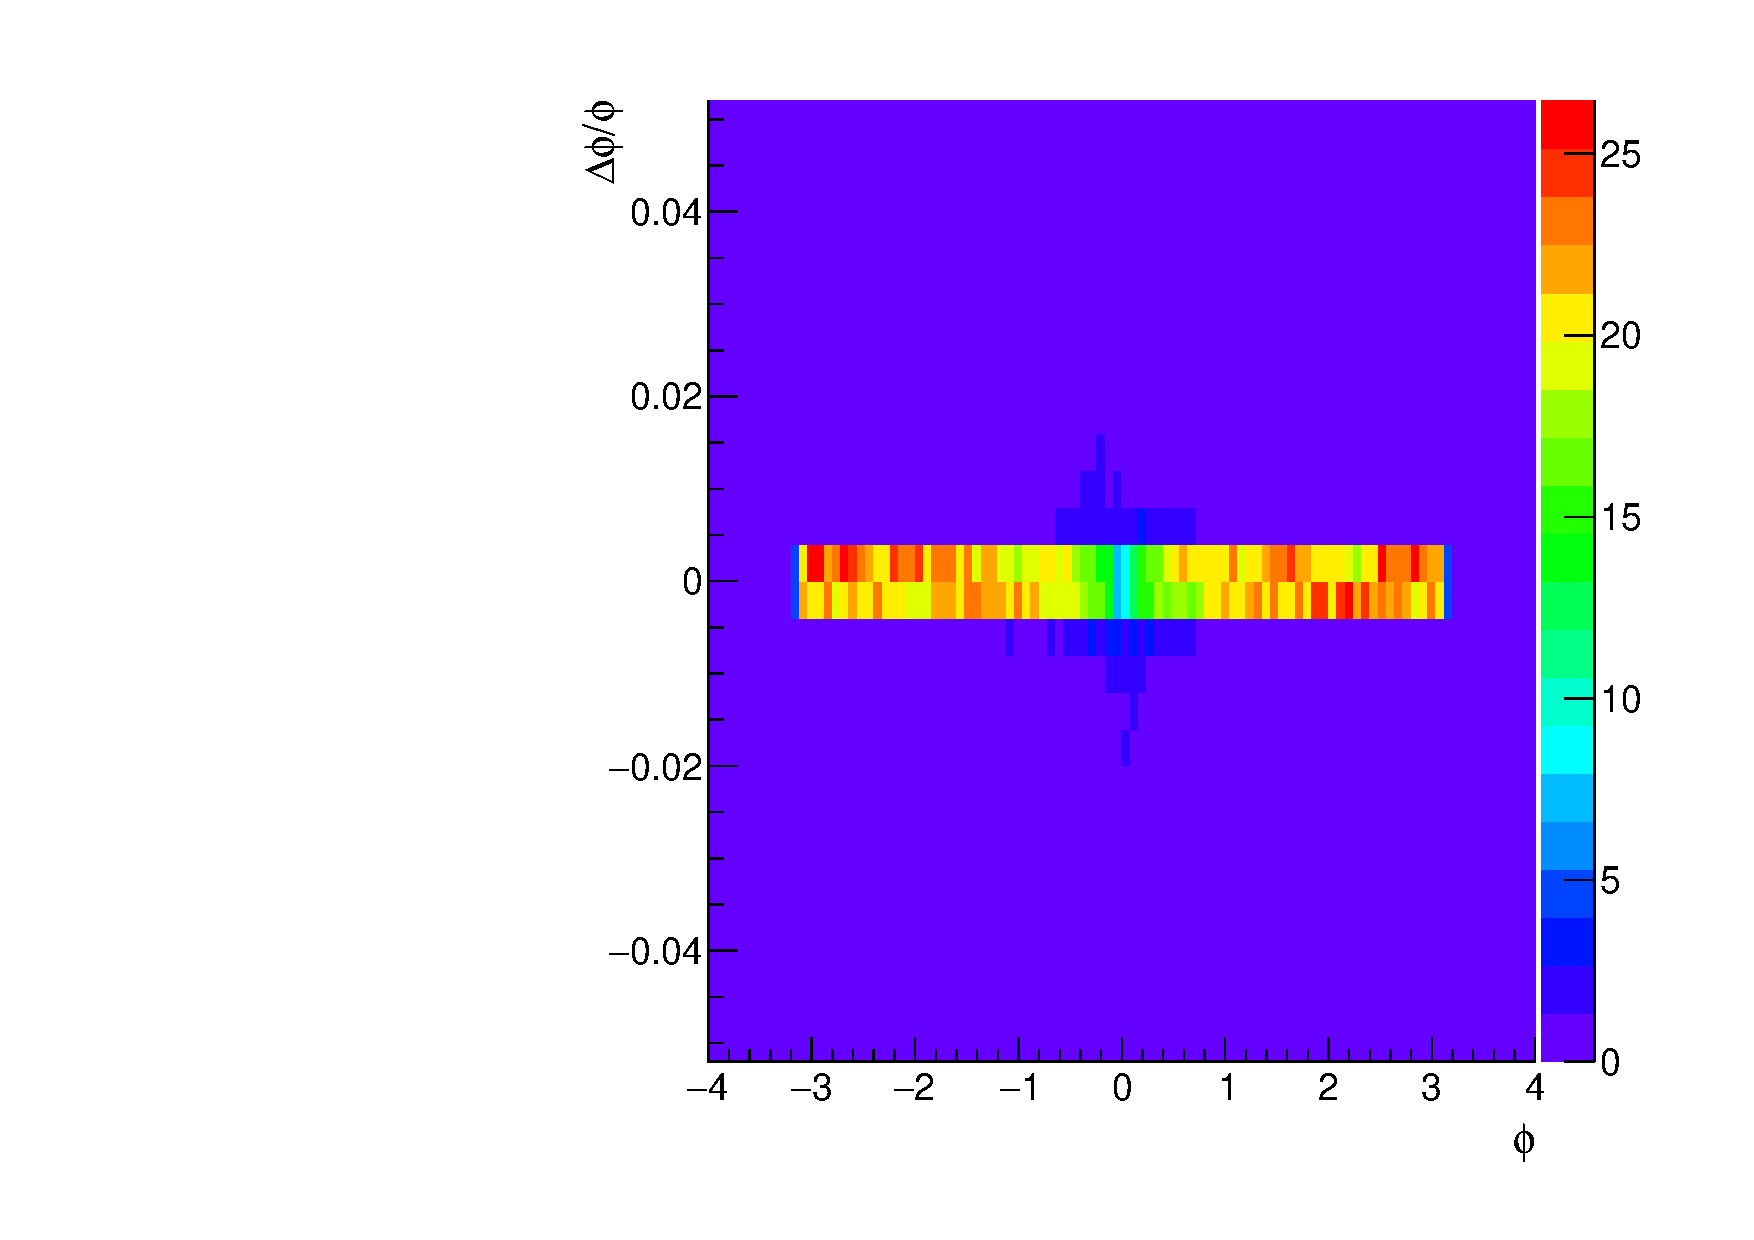
\includegraphics[width=1\linewidth]{phiRatio_Leading_BJet}

			\end{minipage}
			\quad
			\begin{minipage}[h]{0.48\linewidth}
				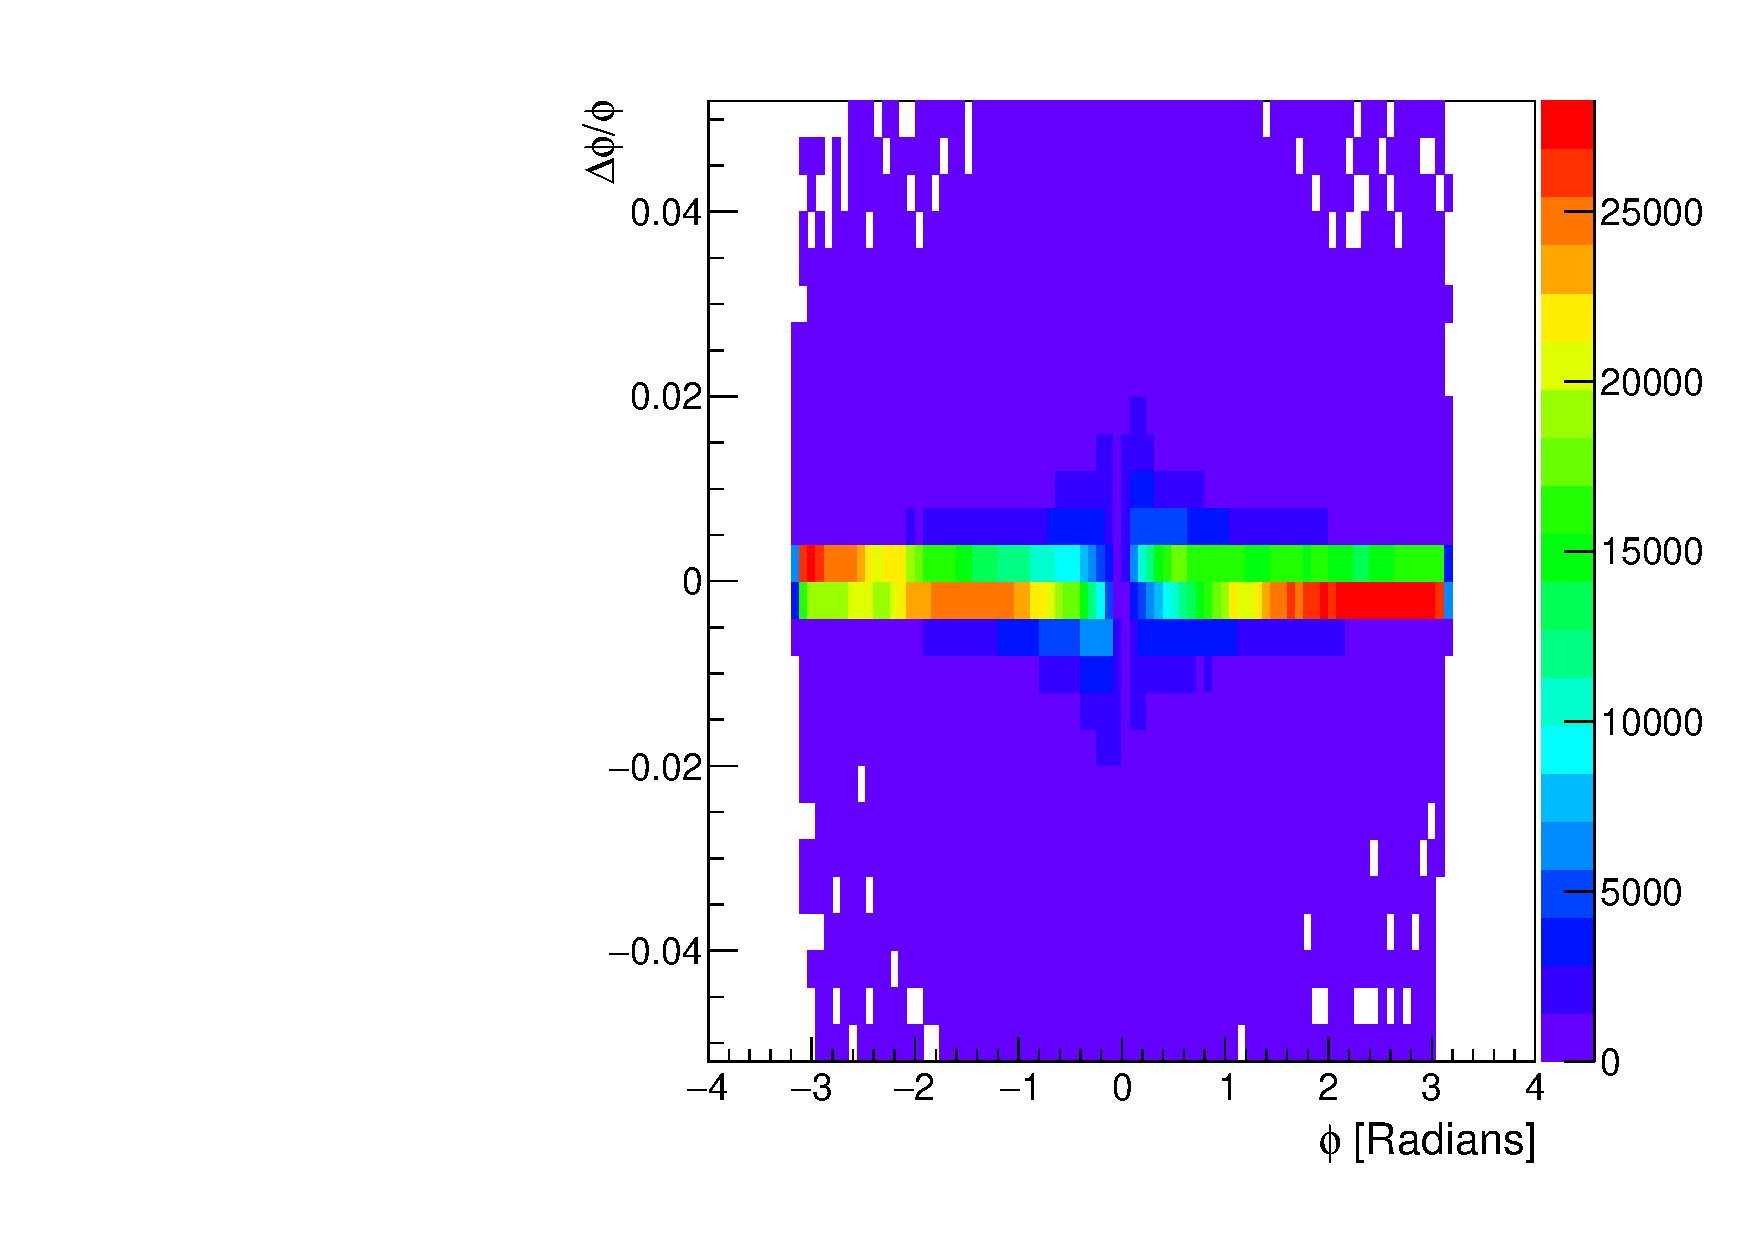
\includegraphics[width=1\linewidth]{Offline_2C_phiRatio_Leading_BJet}
			\end{minipage}
			\caption{\dphph for the leading \bjet, for Monte-Carlo events (left) and real data (right).}
			\label{fig:O:leadingbphi}
		\end{figure}

		The Data and Monte-Carlo distributions for these values are extremely similar to each other, and also show very close agreement between the values for offline and online jet objects. In both cases the median \dxx value is $\sim0$ and the breadth of the distribution is less than $1\%$ of the value.


\newpage
\section{Leading Non \textit{b}-jets}
	\label{OP:leadingnonb}

	For \VBFHBB\, the pair of high \pt forward jets is the other significant feature, so the offline/online performance in the leading non-\bjet was studied.

	\begin{figure}[h]
		\centering
		\begin{minipage}[h]{0.48\linewidth}
			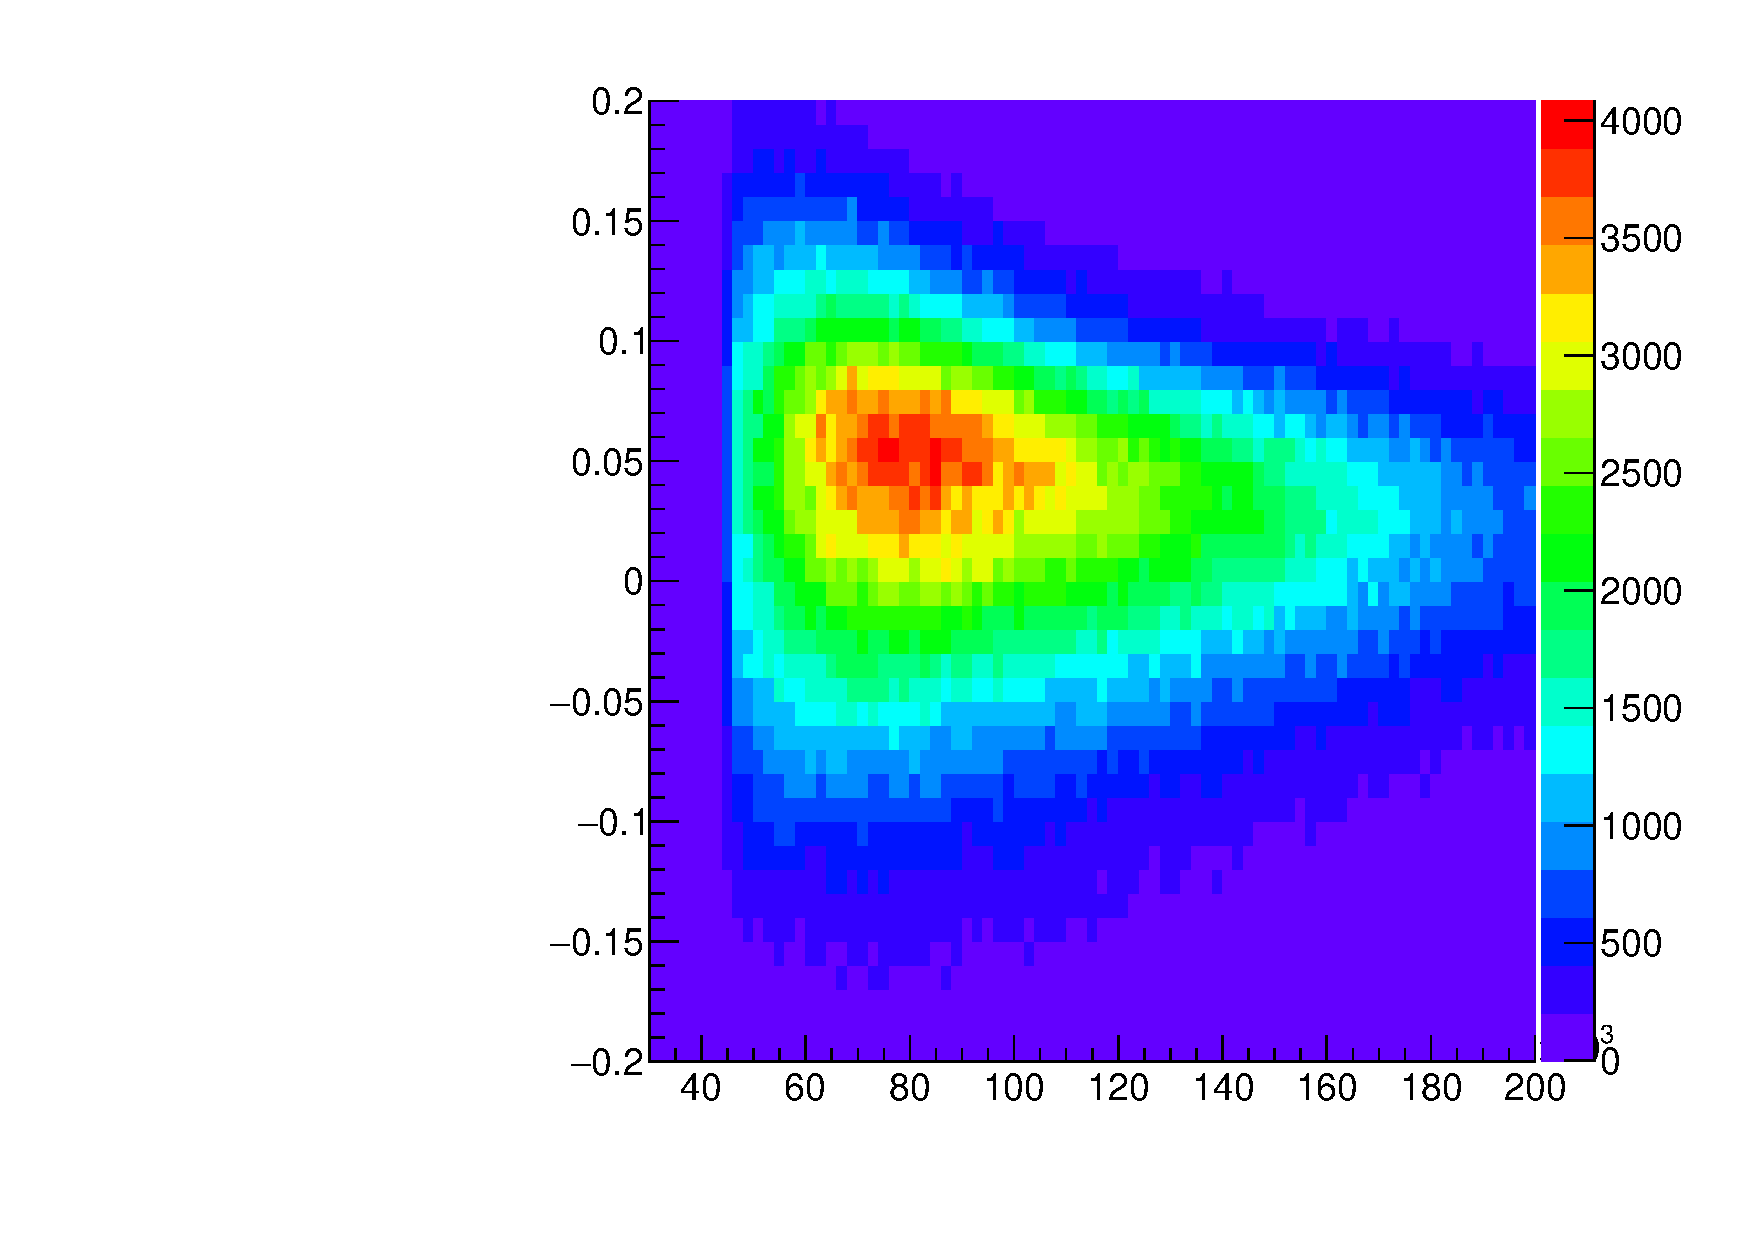
\includegraphics[width=1\linewidth]{ptRatio_Leading_Non_BJet}

		\end{minipage}
		\quad
		\begin{minipage}[h]{0.48\linewidth}
			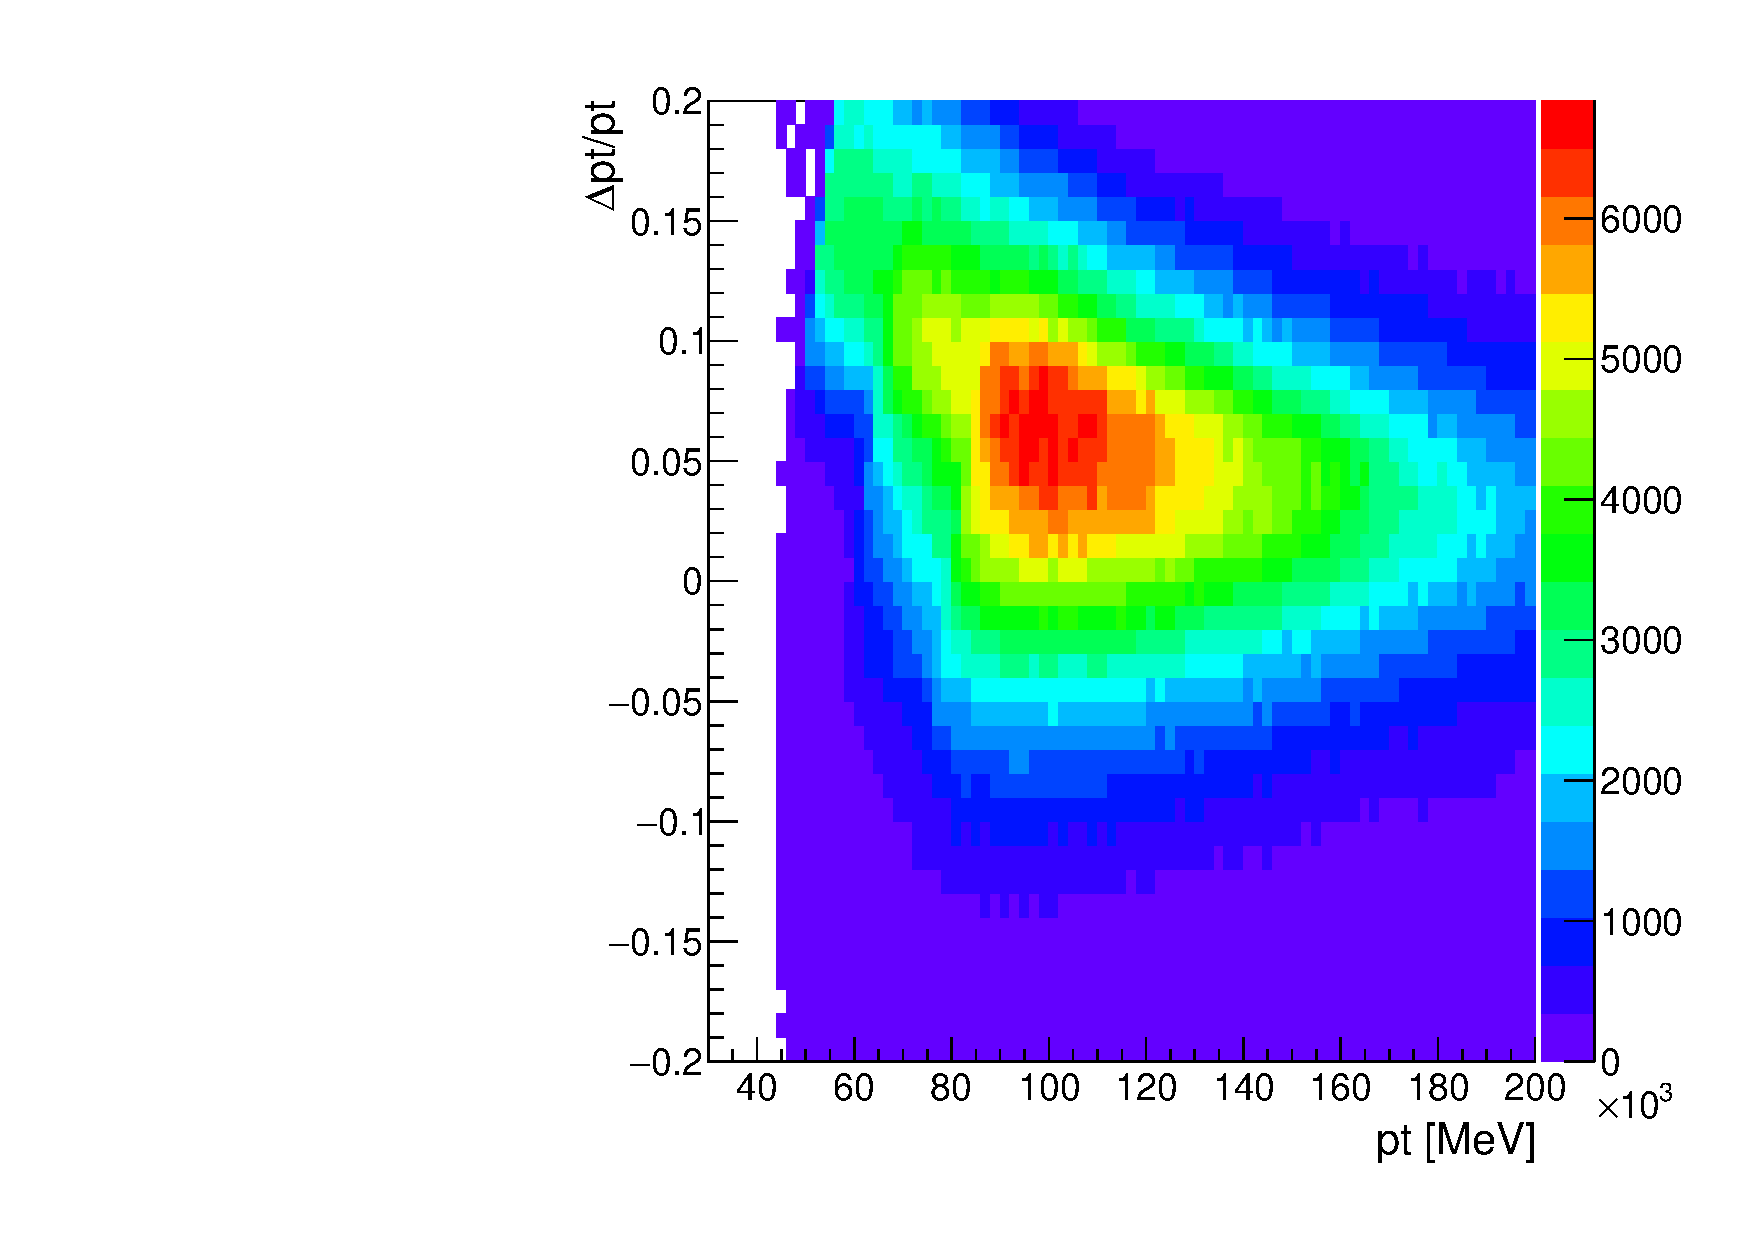
\includegraphics[width=1\linewidth]{Offline_2C_ptRatio_Leading_Non_BJet}
		\end{minipage}
		\caption{\dptpt for the leading \pt non $b$-jet against \pt of the offline jet, plotted for Monte-Carlo simulated results (left) and real data (right).}
		\label{fig:O:leadingnonbpt}
	\end{figure}

	The leading non \bjet\, shows a similar situation to the leading \bjet. At the peak of the \dptpt distribution the \pt of the offline jet is within $5\%$ of the online jet, and the overall shape of the distribution is comparable between the Monte-Carlo and real Data events.
	The results could also be split across $\eta$ regions, with the added ability to study the forward regions of the detector.

	\begin{figure}[h]
		\centering

		\begin{minipage}[h]{0.48\linewidth}
			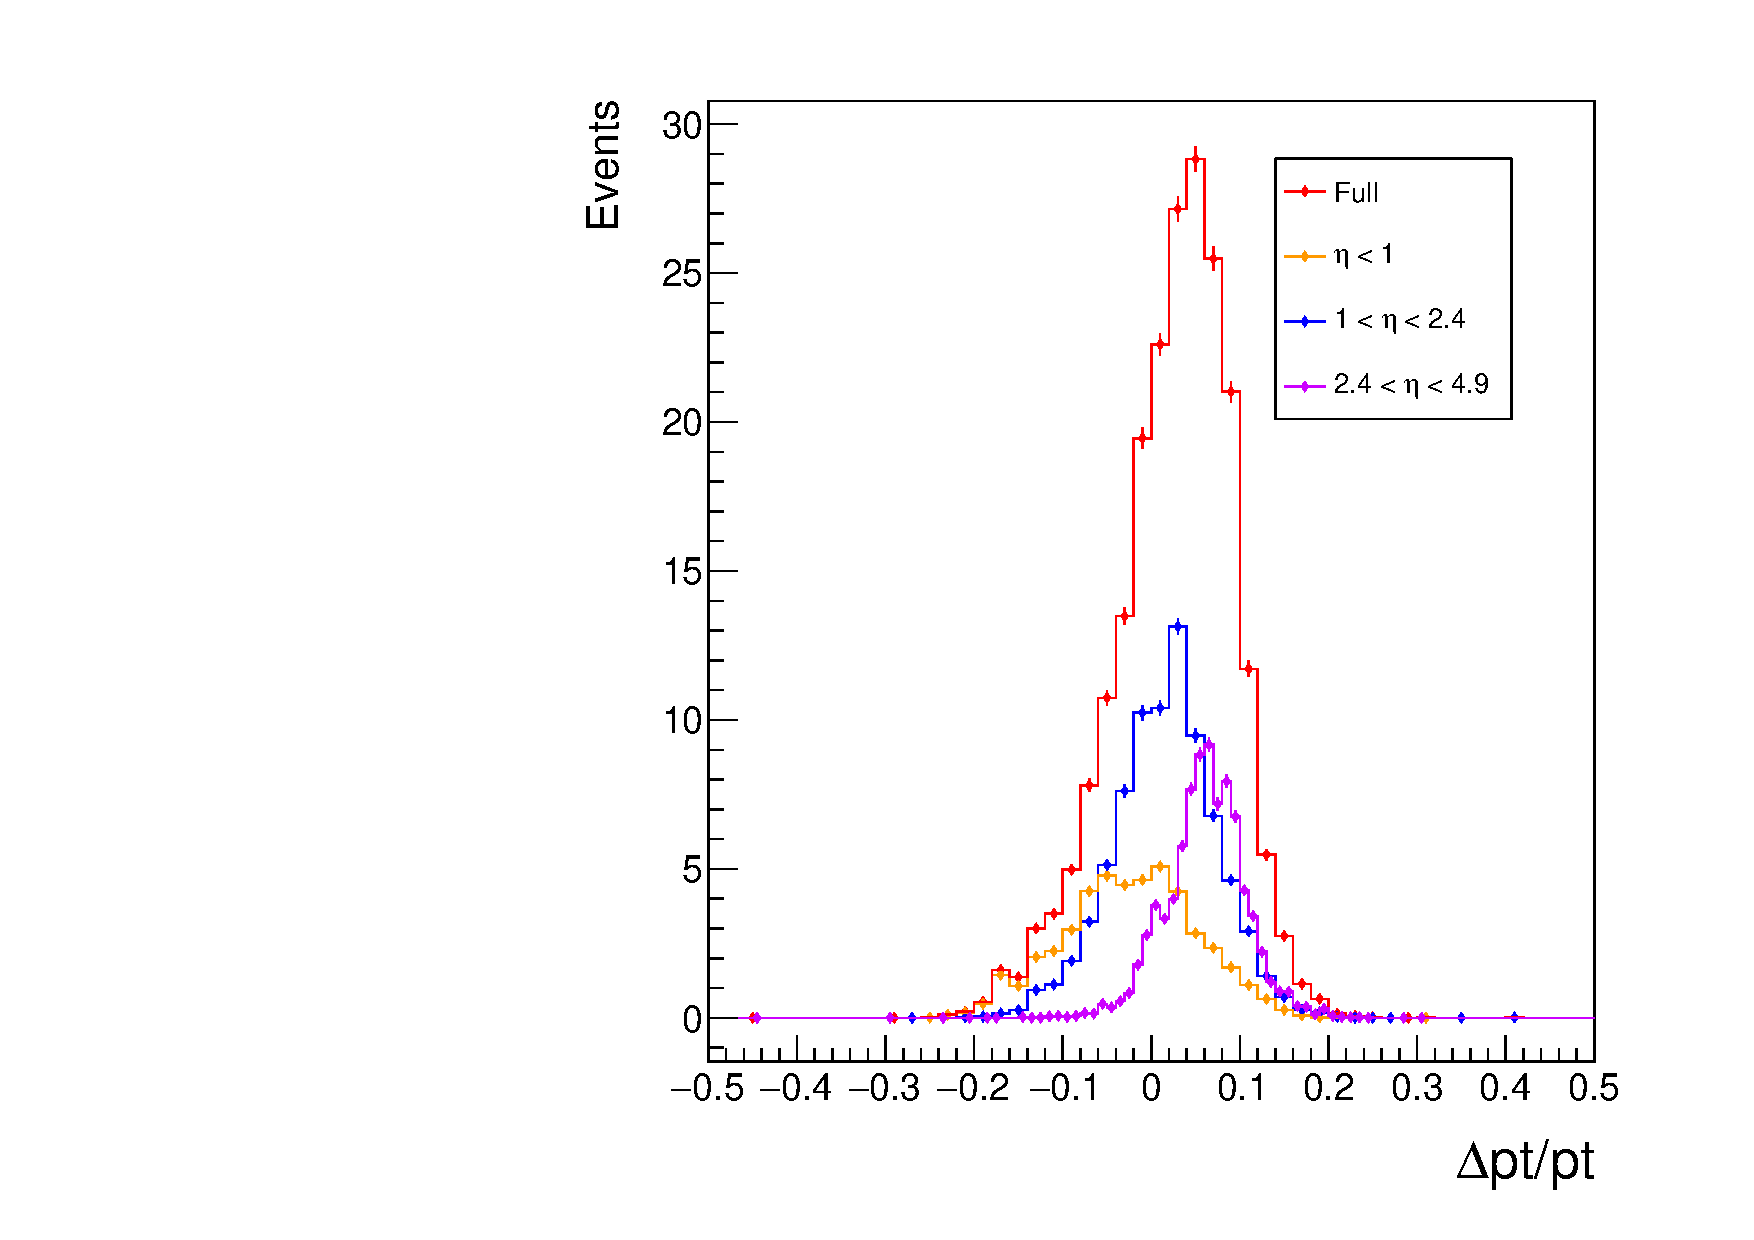
\includegraphics[width=1\linewidth]{Slices_ptRatio_Leading_Non_BJet}
		\end{minipage}
		\quad
		\begin{minipage}[h]{0.48\linewidth}
			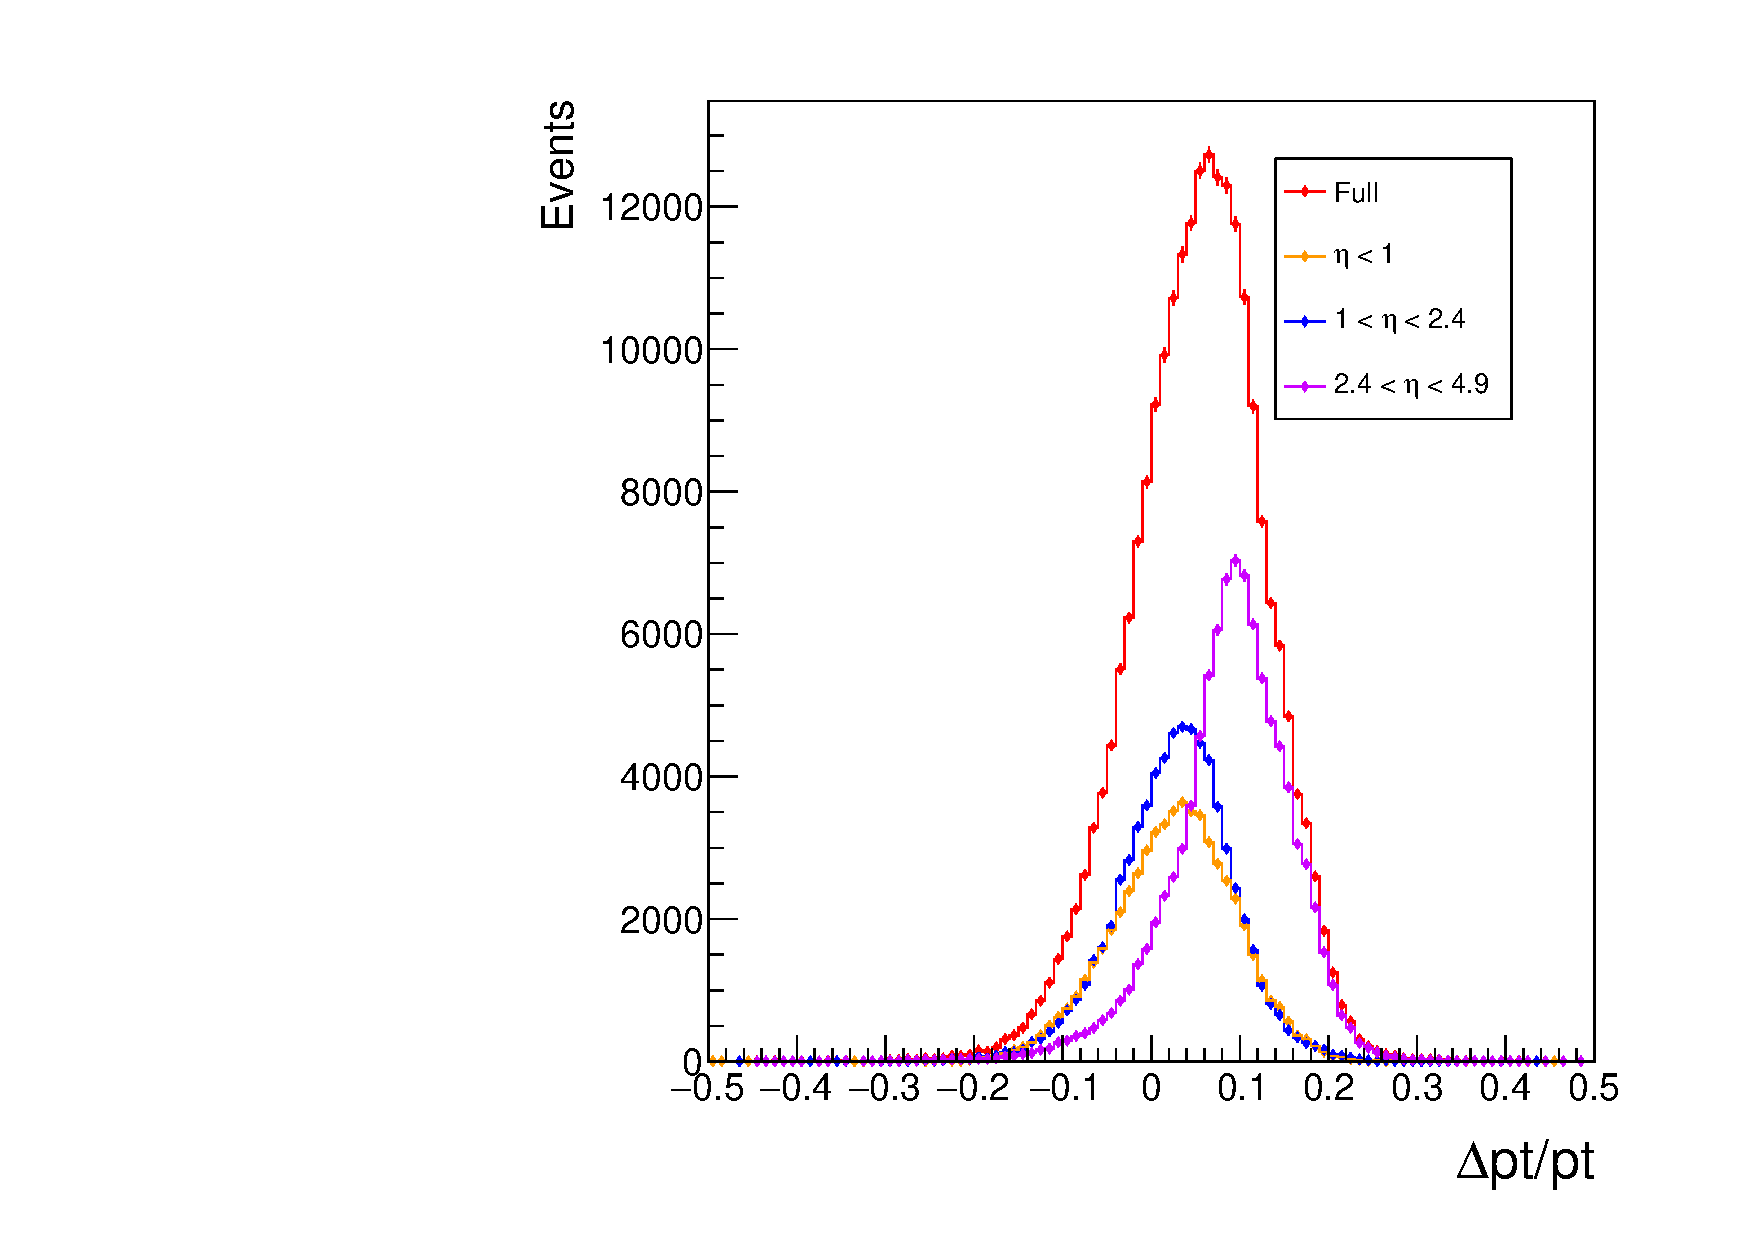
\includegraphics[width=1\linewidth]{Slices_Data_ptRatio_Leading_Non_BJet}
		\end{minipage}
		\caption{\dptpt distribution for the leading non \bjet\, with $89<$\pt$<91$ GeV plotted for Monte-Carlo simulated results (left) and real data (right). The distributions for all events and events split by $\eta$ region are shown.}
		\label{fig:O:leadingnonbptslice}
	\end{figure}

	Both Monte-Carlo and real data show offline jets to be consistently higher \pt than online by $4\%$ and $6\%$ respectively. The overall distribution shape is similar between the simulated and real events for the full set of results, but the distributions for the $\eta$ bands differ between the Monte-Carlo and the real data. The Monte-Carlo results for the central eta band show a dip in \pt at the centre of the distribution and are shifted in \dptpt towards the negative, showing that the online \pt exceeded the offline \pt. In addition, the relative proportions of the three $\eta$ bands differ. The central region of the Monte-Carlo distribution has a flattened peak and peaks at a negative value, showing the offline \pt was less than the online, compared toa positive value for the real data. The Both the MC and the Data show that the offset in \pt value is worse for the jets in the forward region than in the central regions of the detector, with a significantly higher median \dptpt.

	The other topological variables can also be compared.

	\begin{figure}[h]
		\centering
		\begin{minipage}[h]{0.48\linewidth}
			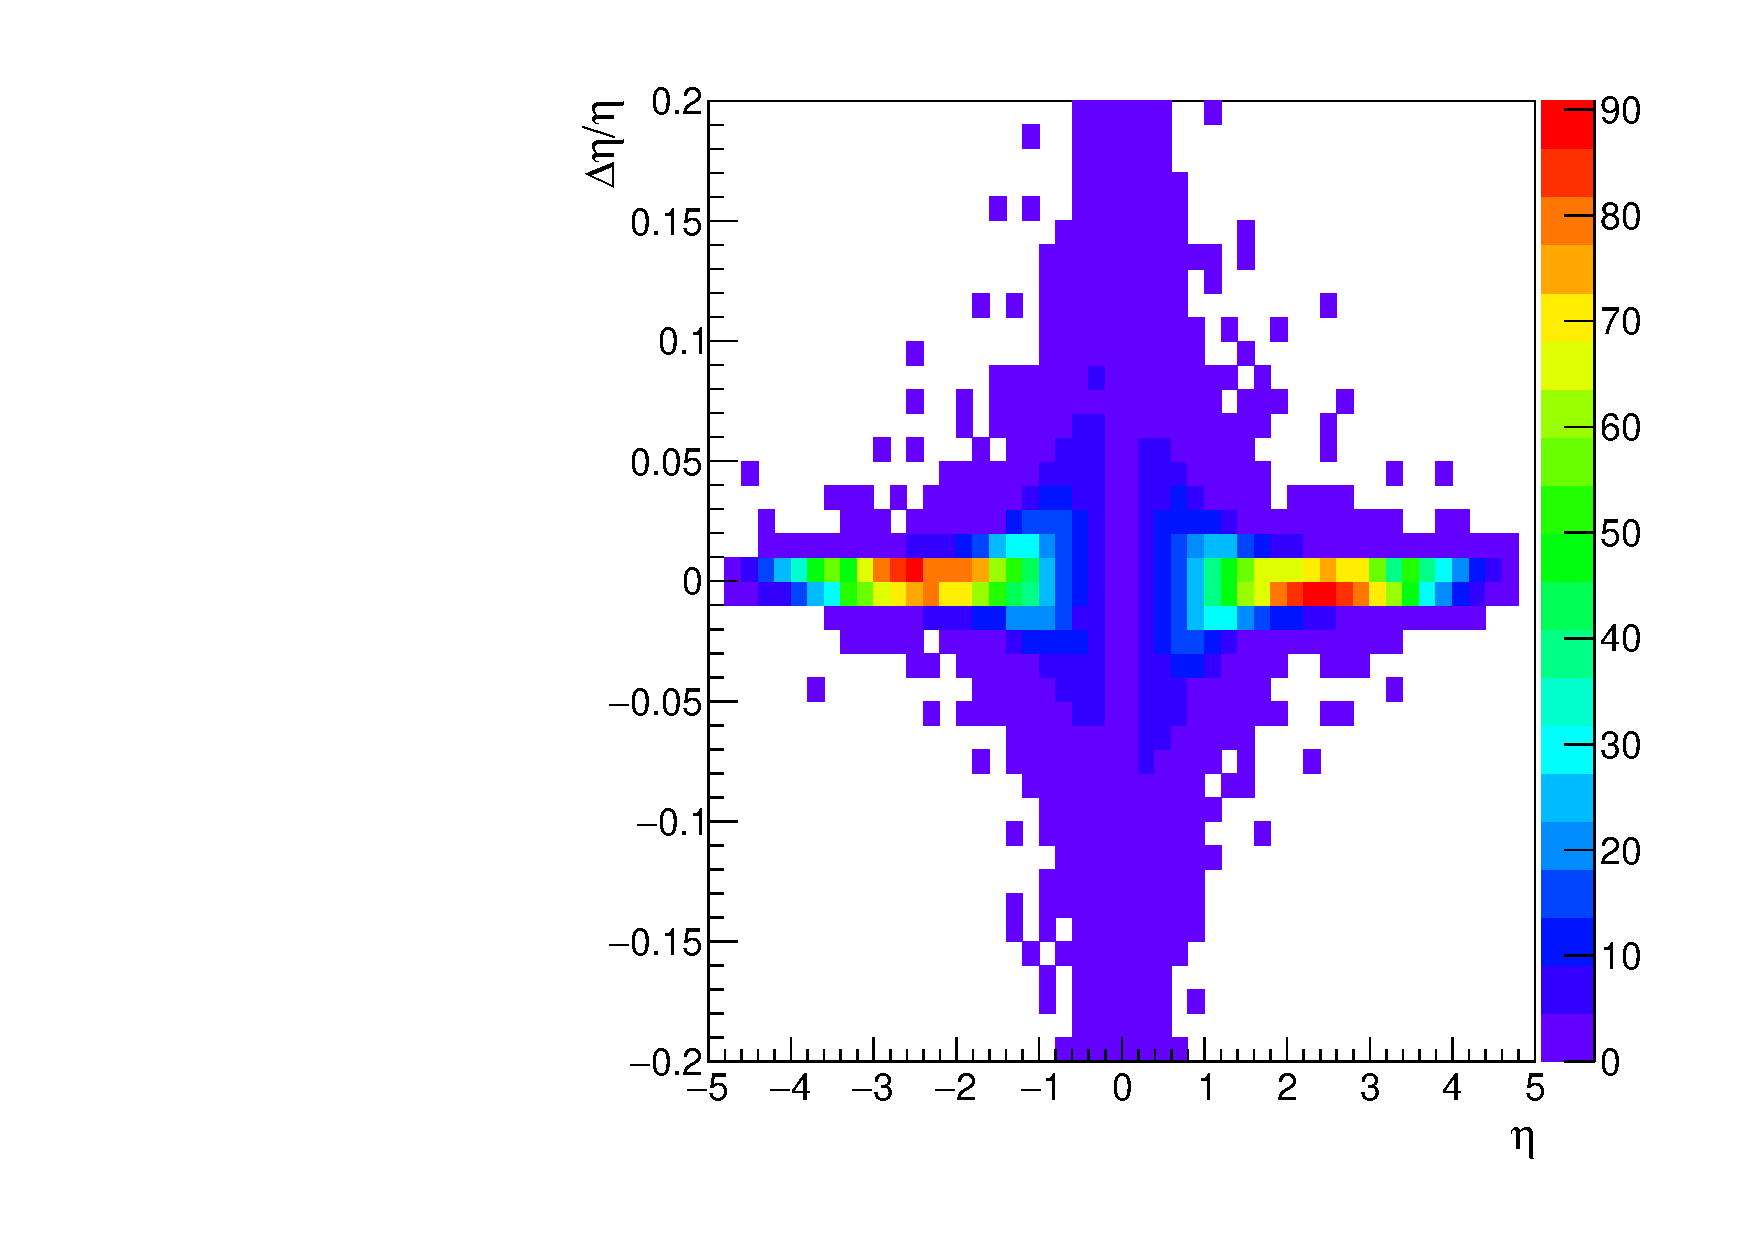
\includegraphics[width=1\linewidth]{etaRatio_Leading_Non_BJet}

		\end{minipage}
		\quad
		\begin{minipage}[h]{0.48\linewidth}
			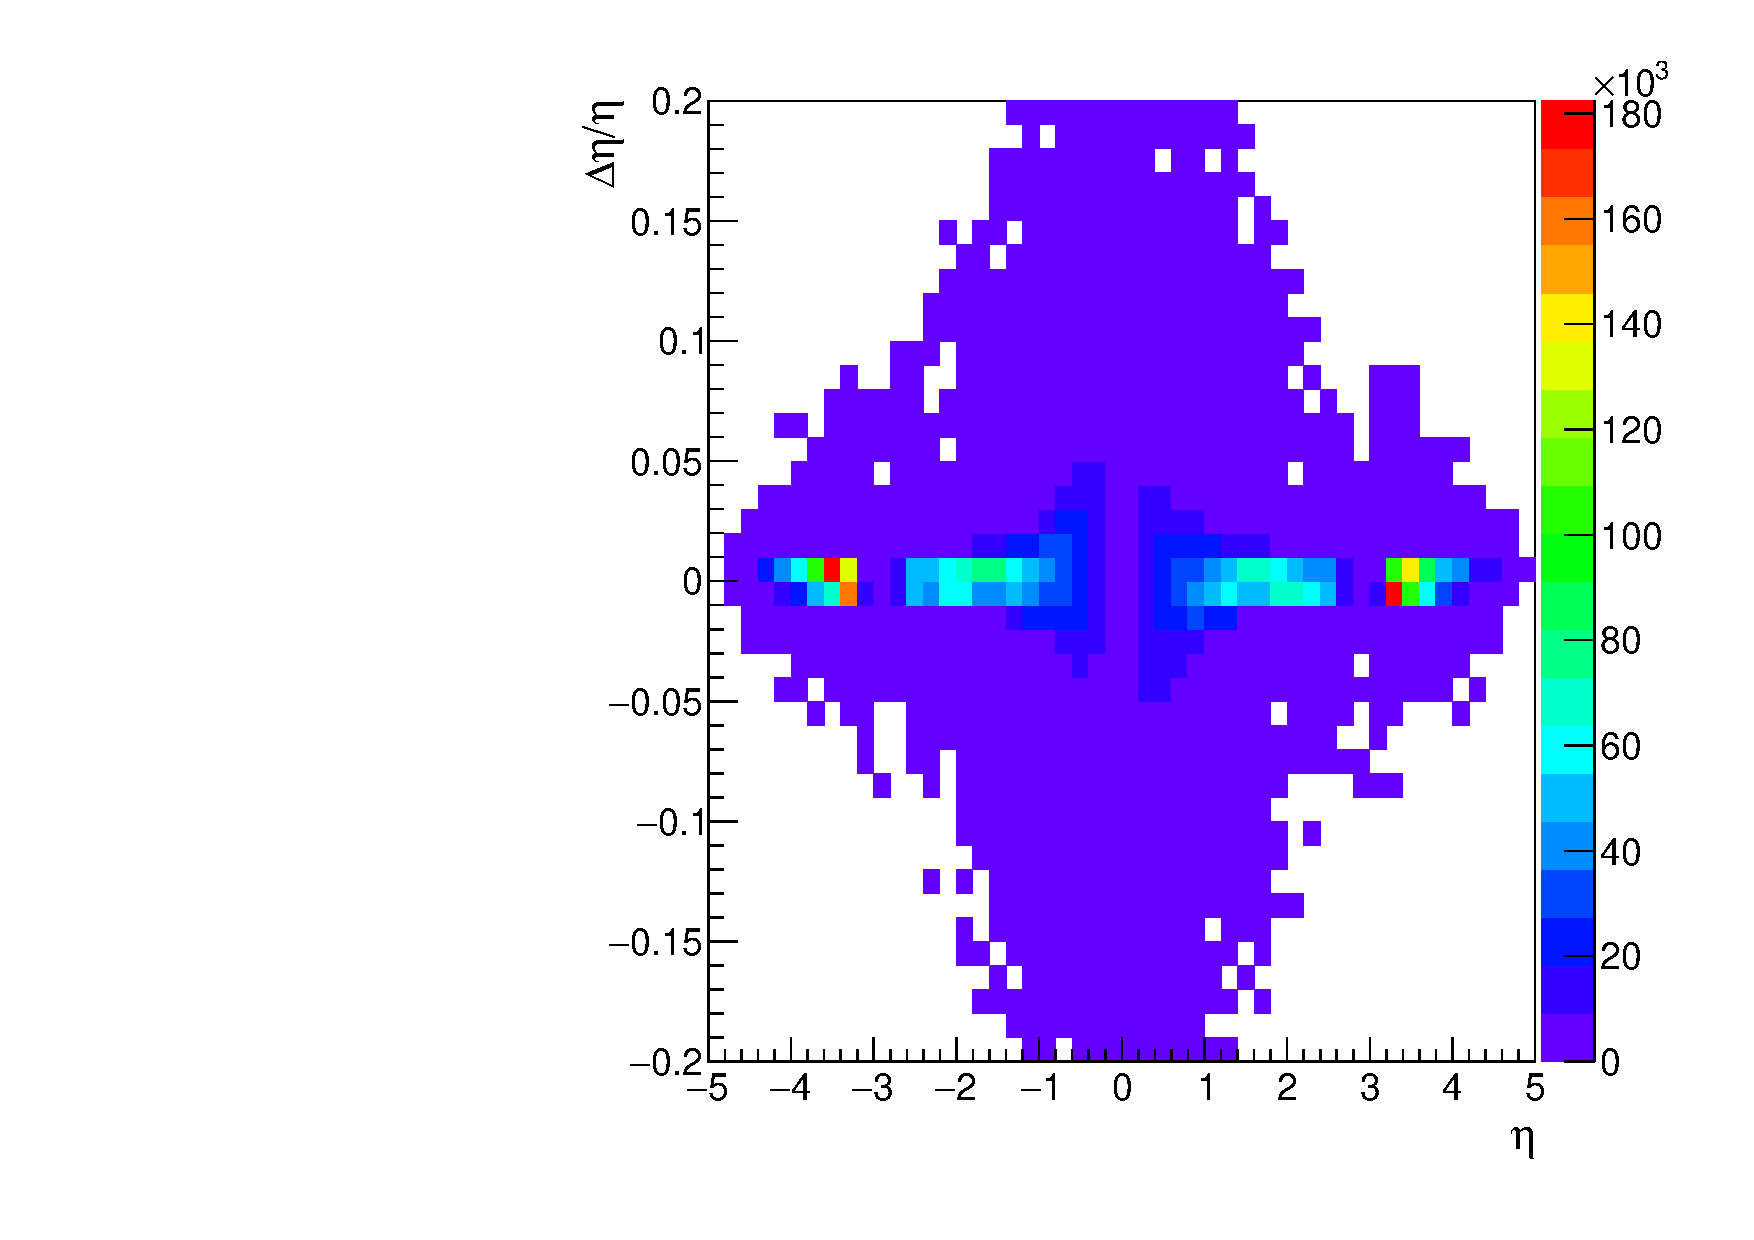
\includegraphics[width=1\linewidth]{Offline_2C_etaRatio_Leading_Non_BJet}
		\end{minipage}
		\caption{\dee for the leading non \bjet, for Monte-Carlo events (left) and real data (right).}
		\label{fig:O:leadingnonbeta}
	\end{figure}

	\begin{figure}[h]
		\centering
		\begin{minipage}[h]{0.48\linewidth}
			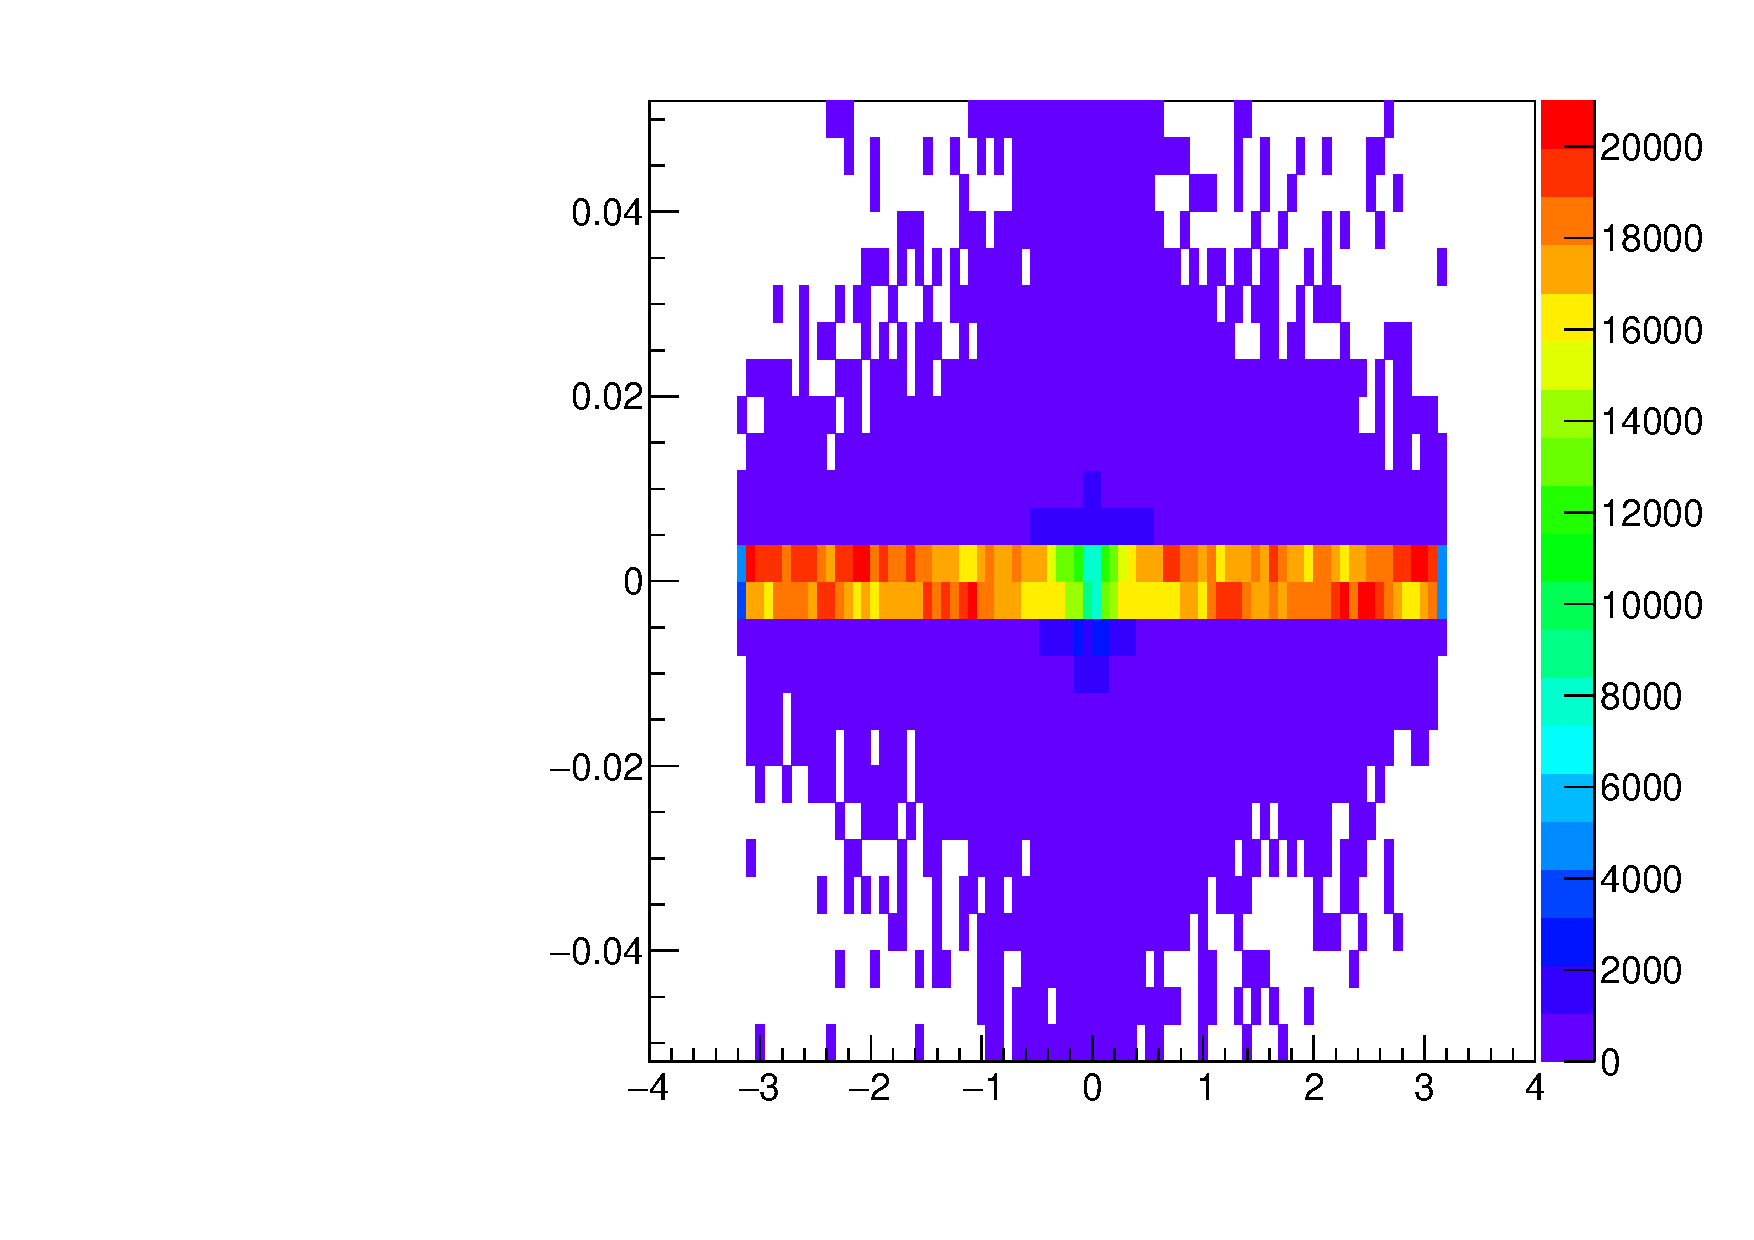
\includegraphics[width=1\linewidth]{phiRatio_Leading_Non_BJet}

		\end{minipage}
		\quad
		\begin{minipage}[h]{0.48\linewidth}
			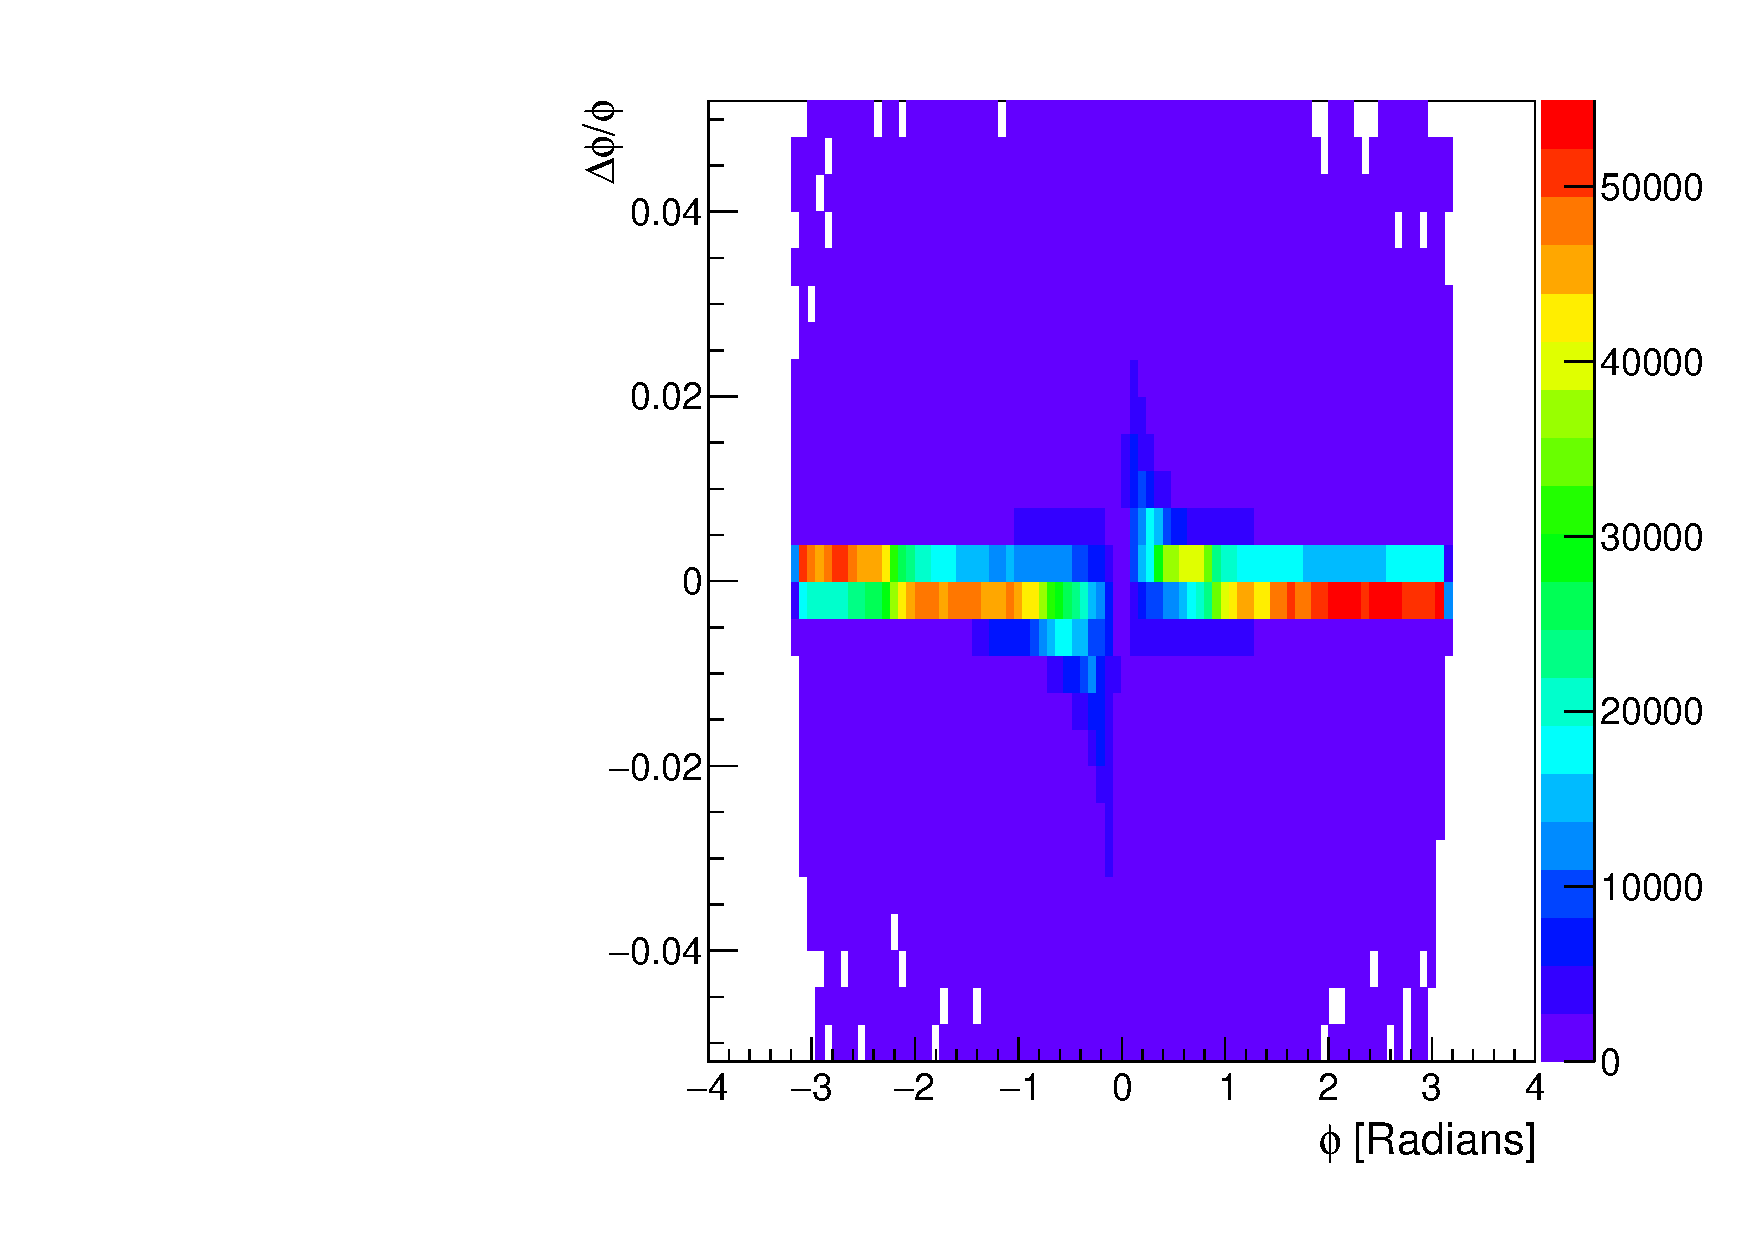
\includegraphics[width=1\linewidth]{Offline_2C_phiRatio_Leading_Non_BJet}
		\end{minipage}
		\caption{\dphph for the leading non \bjet, for Monte-Carlo events (left) and real data (right)}
		\label{fig:O:leadingnonbphi}
	\end{figure}

	As with the \bjets\, these other variables offline and online jets produce nearly identical results, with the distribution of \dxx firmly centred around 0 and a breadth of less than $1\%$.

	\subsection{Comparison of Jet Objects between Offline and Online}

		The jet objects reconstructed in the HLT have some slight differences in the reported values for key topological variables, but overall they perform in a similar fashion, both in Monte-Carlo simulations and in Real data. The positional variables, $\phi$ and $\eta$ are directly comparable between offline and online jet objects, with the majority of objects having values with $<1\%$ disagreement for both \bjets\, and non \bjets\,. For the \pt of jet objects, the values are not in perfect agreement, but have a consistent offset observed in Monte-Carlo and Real data which could be overcome with specific calibration of the jet objects reconstructed in the HLT.

\section{Jet Tagging Efficiency}

	As covered in Section  \ref{det:btag:mv}, the standard algorithm for 2016 physics analyses was chosen to be the 2016 MV2c10 algorithm. However, the HLT \btag\, algorithm uses the MV2c20 algorithm \cite{trig2015}. In order for any form a Trigger Level Analysis to be considered valid, the performance of the tagging algorithms used in the trigger, which are fixed at the point of data collection, must be comparable with the tagging executed offline with more up to date \btag\, configurations.

	To study this, the \btag\, efficiency at trigger level and offline is studied for different jet flavours using the MC sample. The Monte-Carlo sample was used as being generated rather than recorded the \textit{truth} nature of the jet object was known, and the result of the \btag\, algorithm can be compared to this truth label. This requirement for a truth label means only Monte-Carlo data can be used for this comparison.

	In the analysis, an offline/HLT jet pair was formed using $\Delta R$ matching and truth label of the offline jet used to assign a flavour to the pair. Light-jets, \bjets\, and \cjets\, were all studied separately to view the \btag\, efficiency and the mistag rate of both algorithms operating at the \textit{tight} working point. The efficiency plots in Figures \ref{fig:MC:bjetefficiency}, \ref{fig:MC:cjetefficiency} and \ref{fig:MC:lightjetefficiency} show the fraction of these jets that were identified as \bjets\, by the HLT and offline tagging algorithms.

	\newpage
	\subsection{\textit{b}-jet efficiency}

	For jets labelled as true \bjets, the tagging efficiency can be calculated and plotted with respect to topological variables of the jet objects.

		\begin{figure}[h]
			\centering
			\begin{minipage}[h]{0.48\linewidth}
				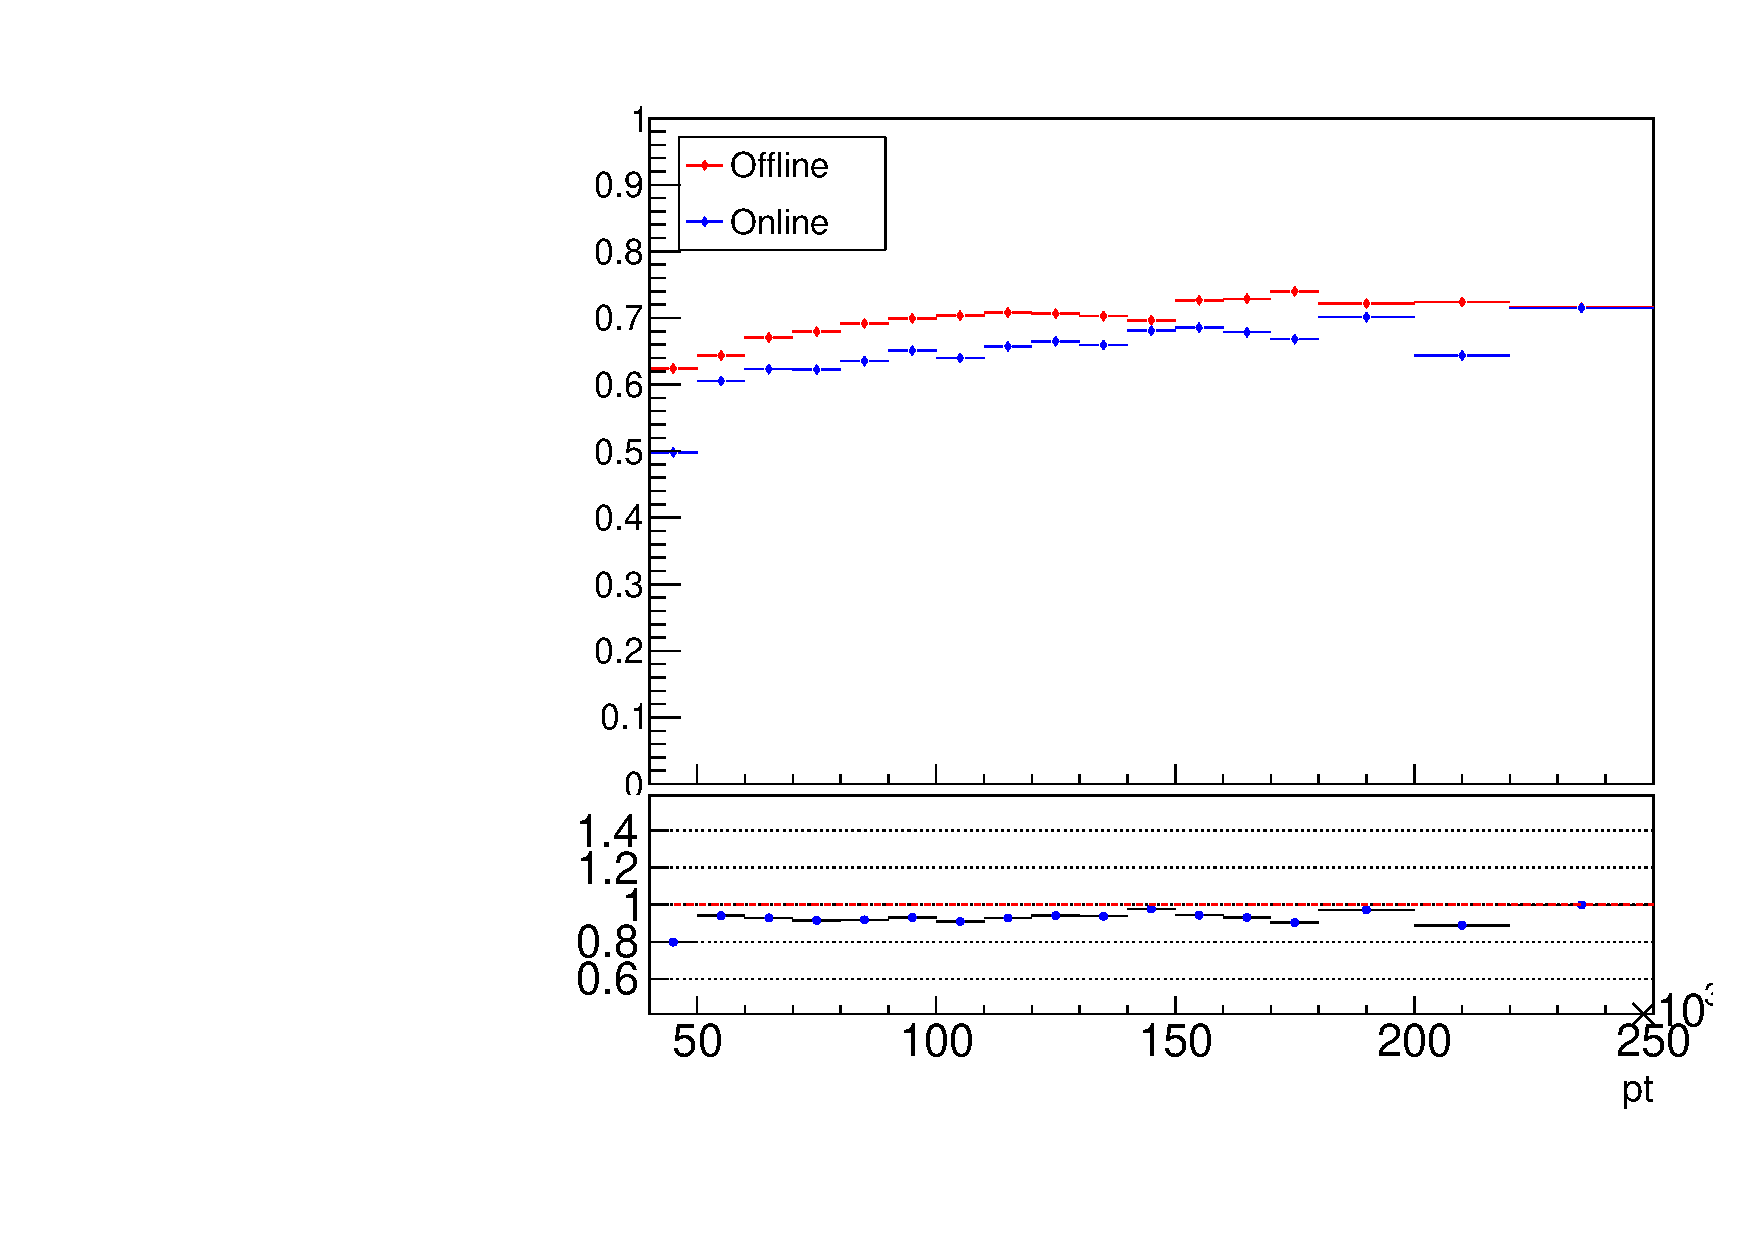
\includegraphics[width=1\linewidth]{ptBJET}

			\end{minipage}
			\quad
			\begin{minipage}[h]{0.48\linewidth}
				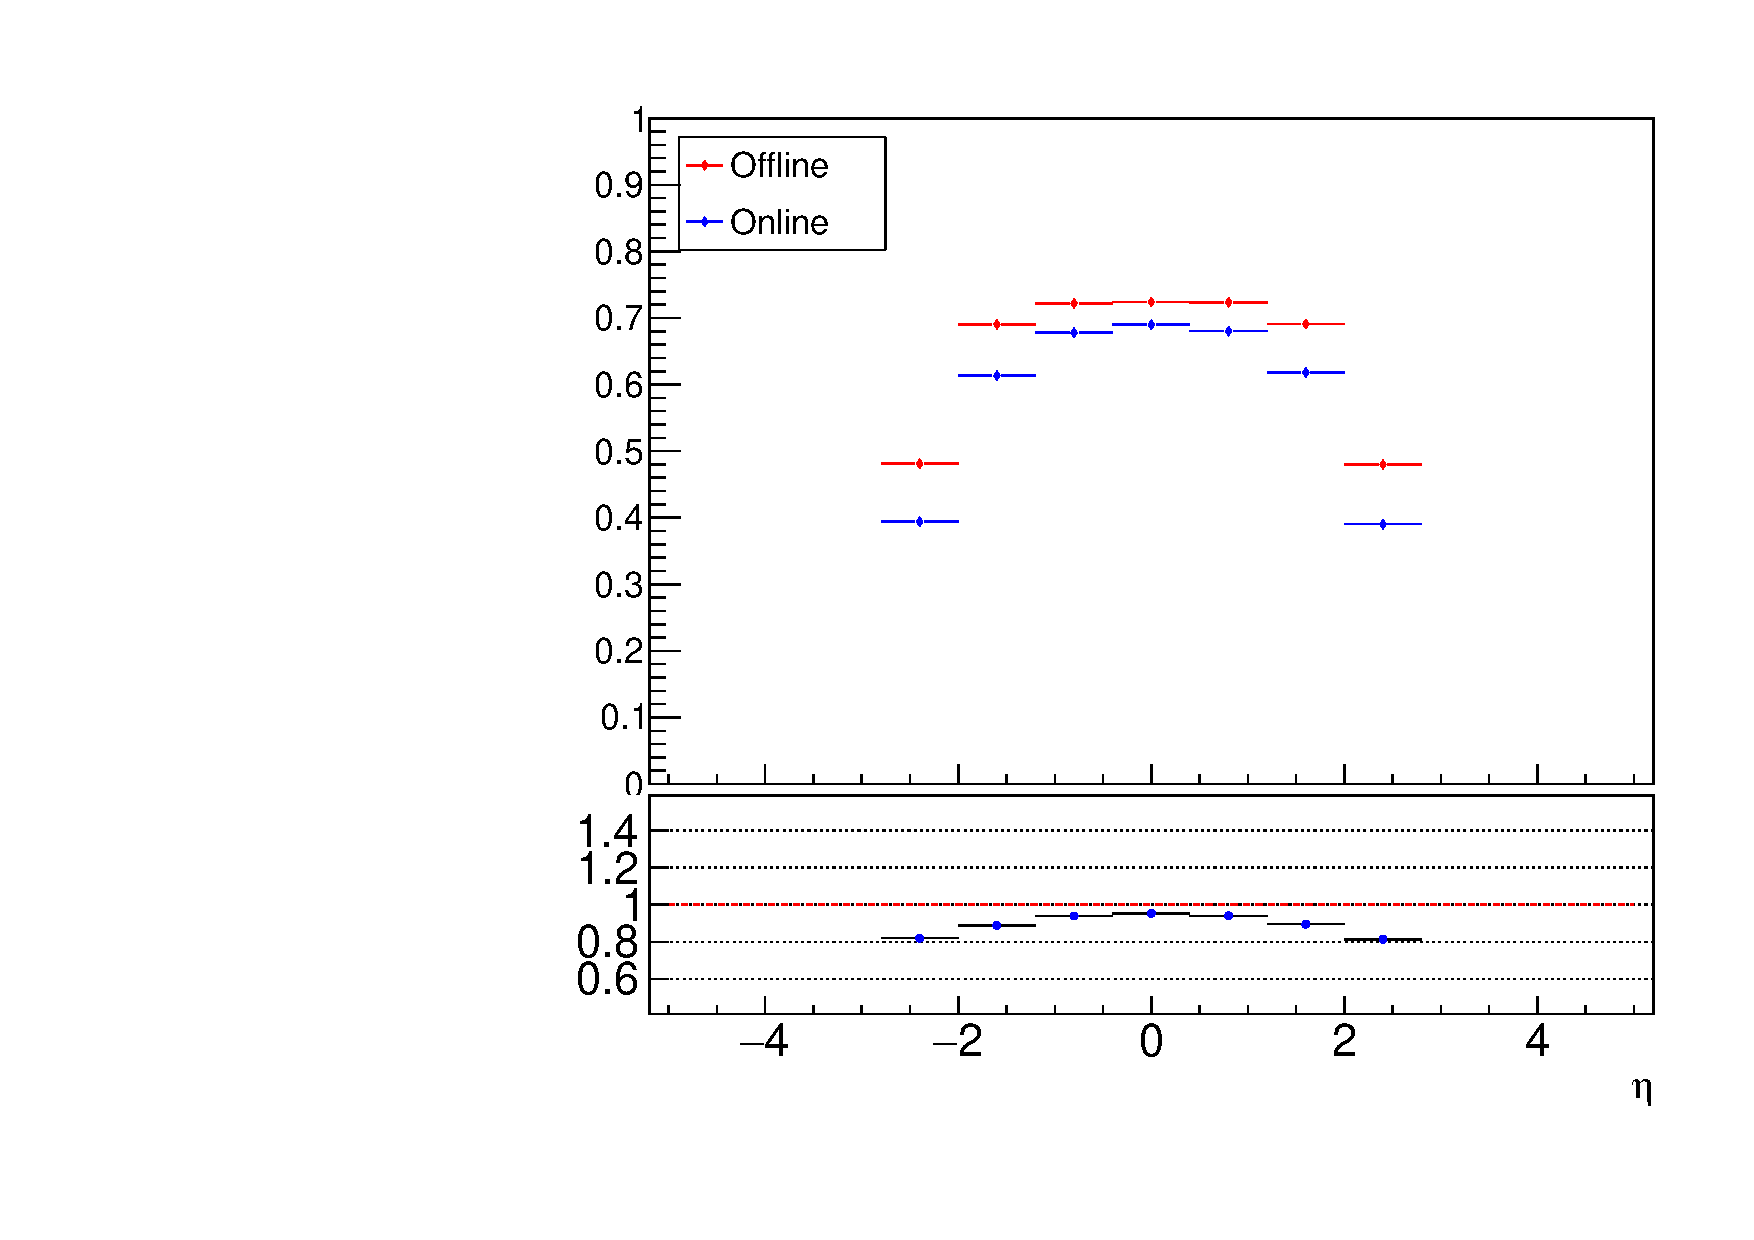
\includegraphics[width=1\linewidth]{etaBJET}
			\end{minipage}
			\caption{\btag\, efficiency for truth \bjets\, in Monte-Carlo data, plotted against jet \pt (left) and $\eta$ (right).}
			\label{fig:MC:bjetefficiency}
		\end{figure}

	\subsection{\textit{c}-jet efficiency}
	For \cjets\, and light-jets, plotting the same value gives the mistag rate for these jets in the detector.

		\begin{figure}[h]
			\centering
			\begin{minipage}[h]{0.48\linewidth}
				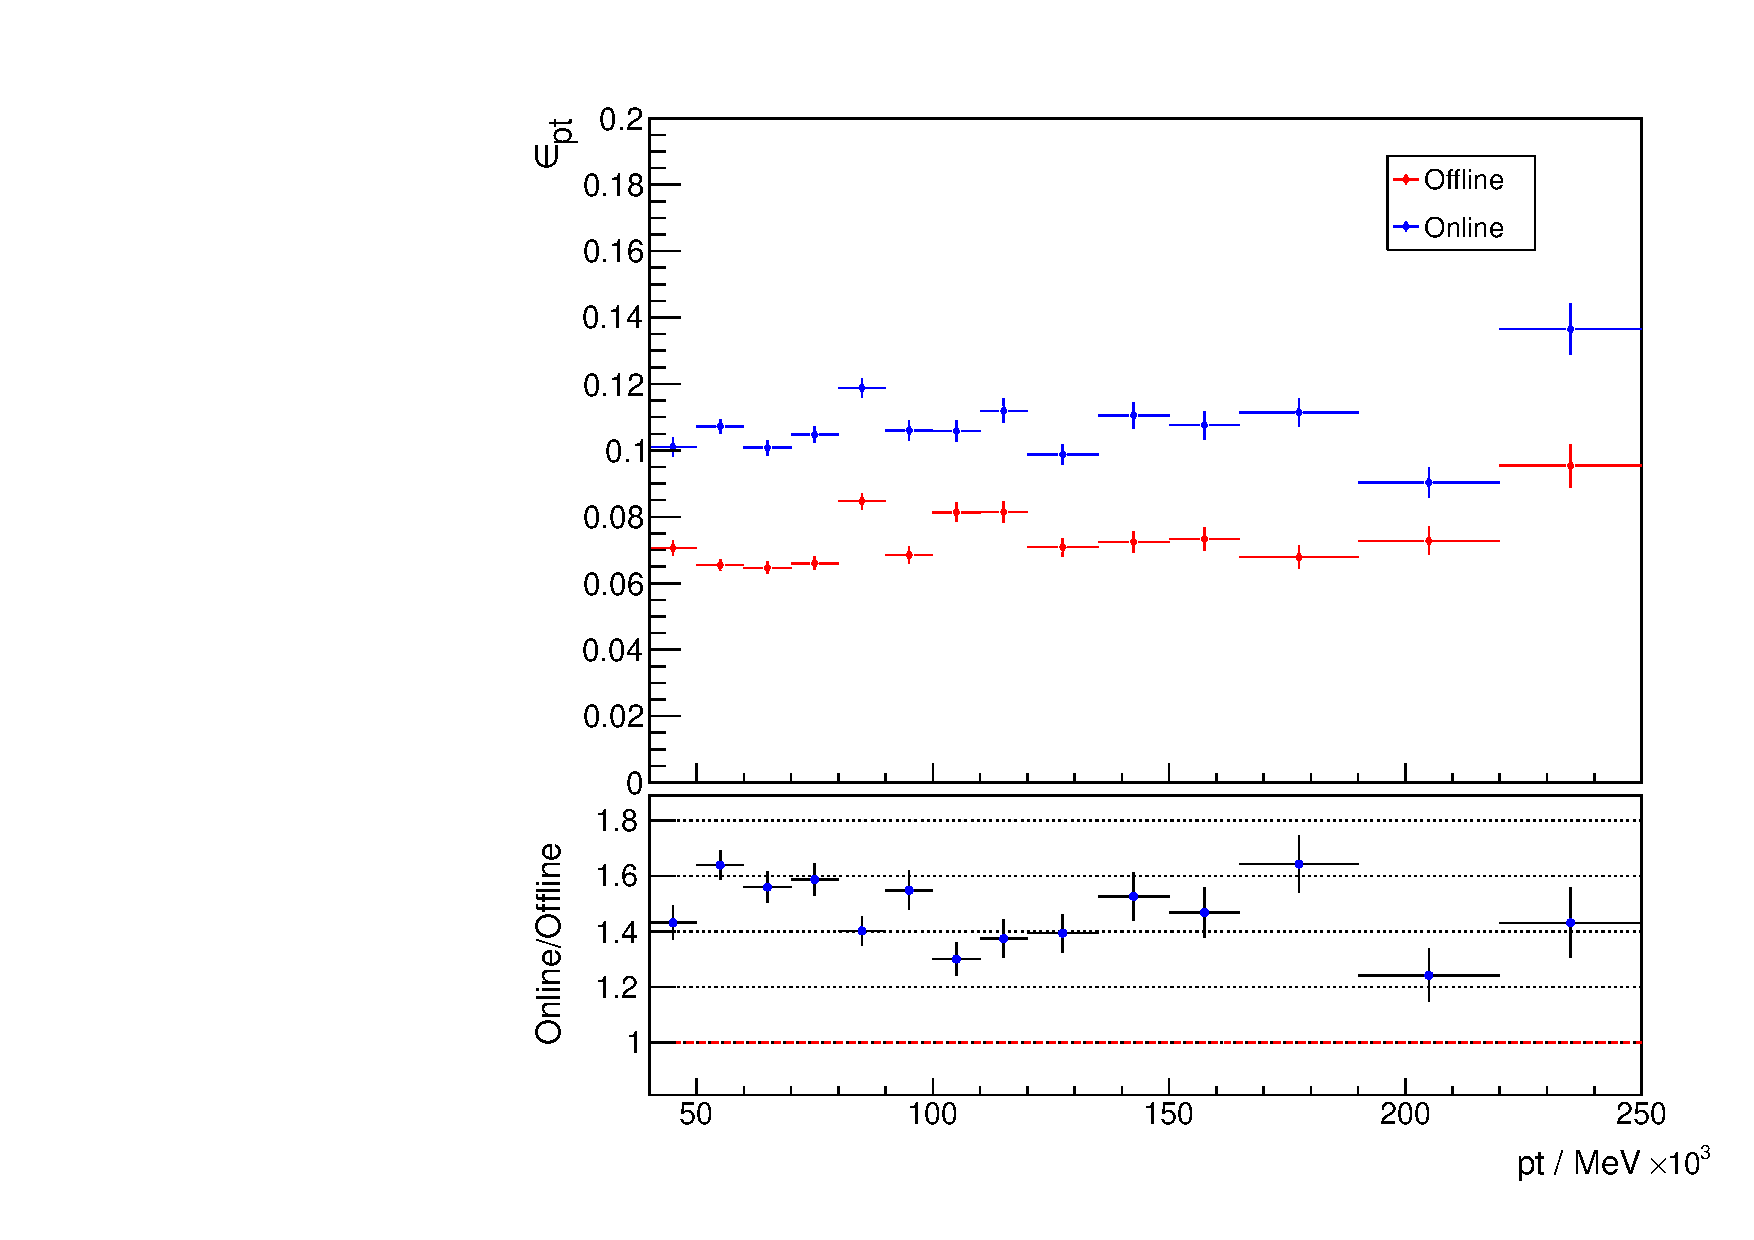
\includegraphics[width=1\linewidth]{ptCJET}

			\end{minipage}
			\quad
			\begin{minipage}[h]{0.48\linewidth}
				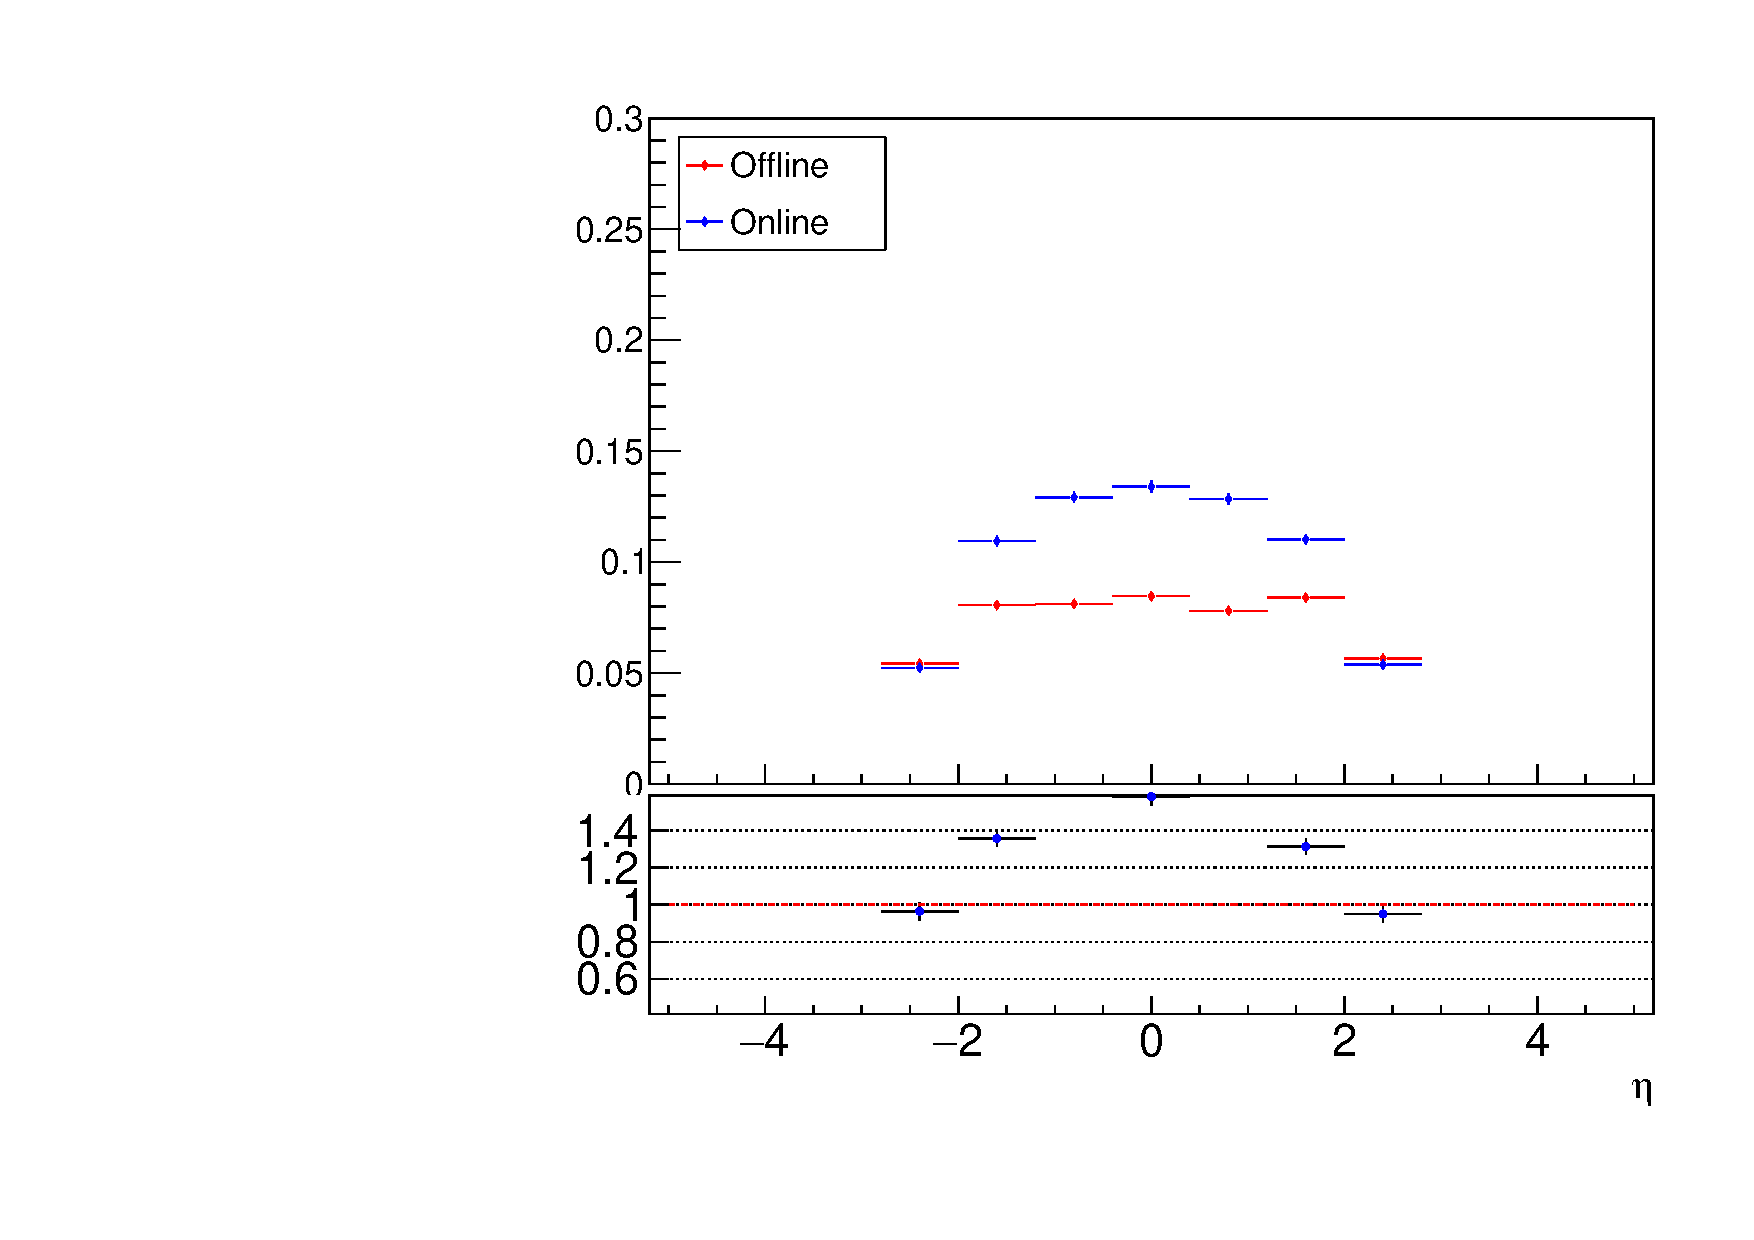
\includegraphics[width=1\linewidth]{etaCJET}
			\end{minipage}
			\caption{Mistag rate for truth \bjets\, in Monte-Carlo data, plotted against jet \pt (left) and $\eta$ (right).}
			\label{fig:MC:cjetefficiency}
		\end{figure}

\newpage
	\subsection{Light-jet efficiency}

		\begin{figure}[h]
			\centering
			\begin{minipage}[h]{0.48\linewidth}
				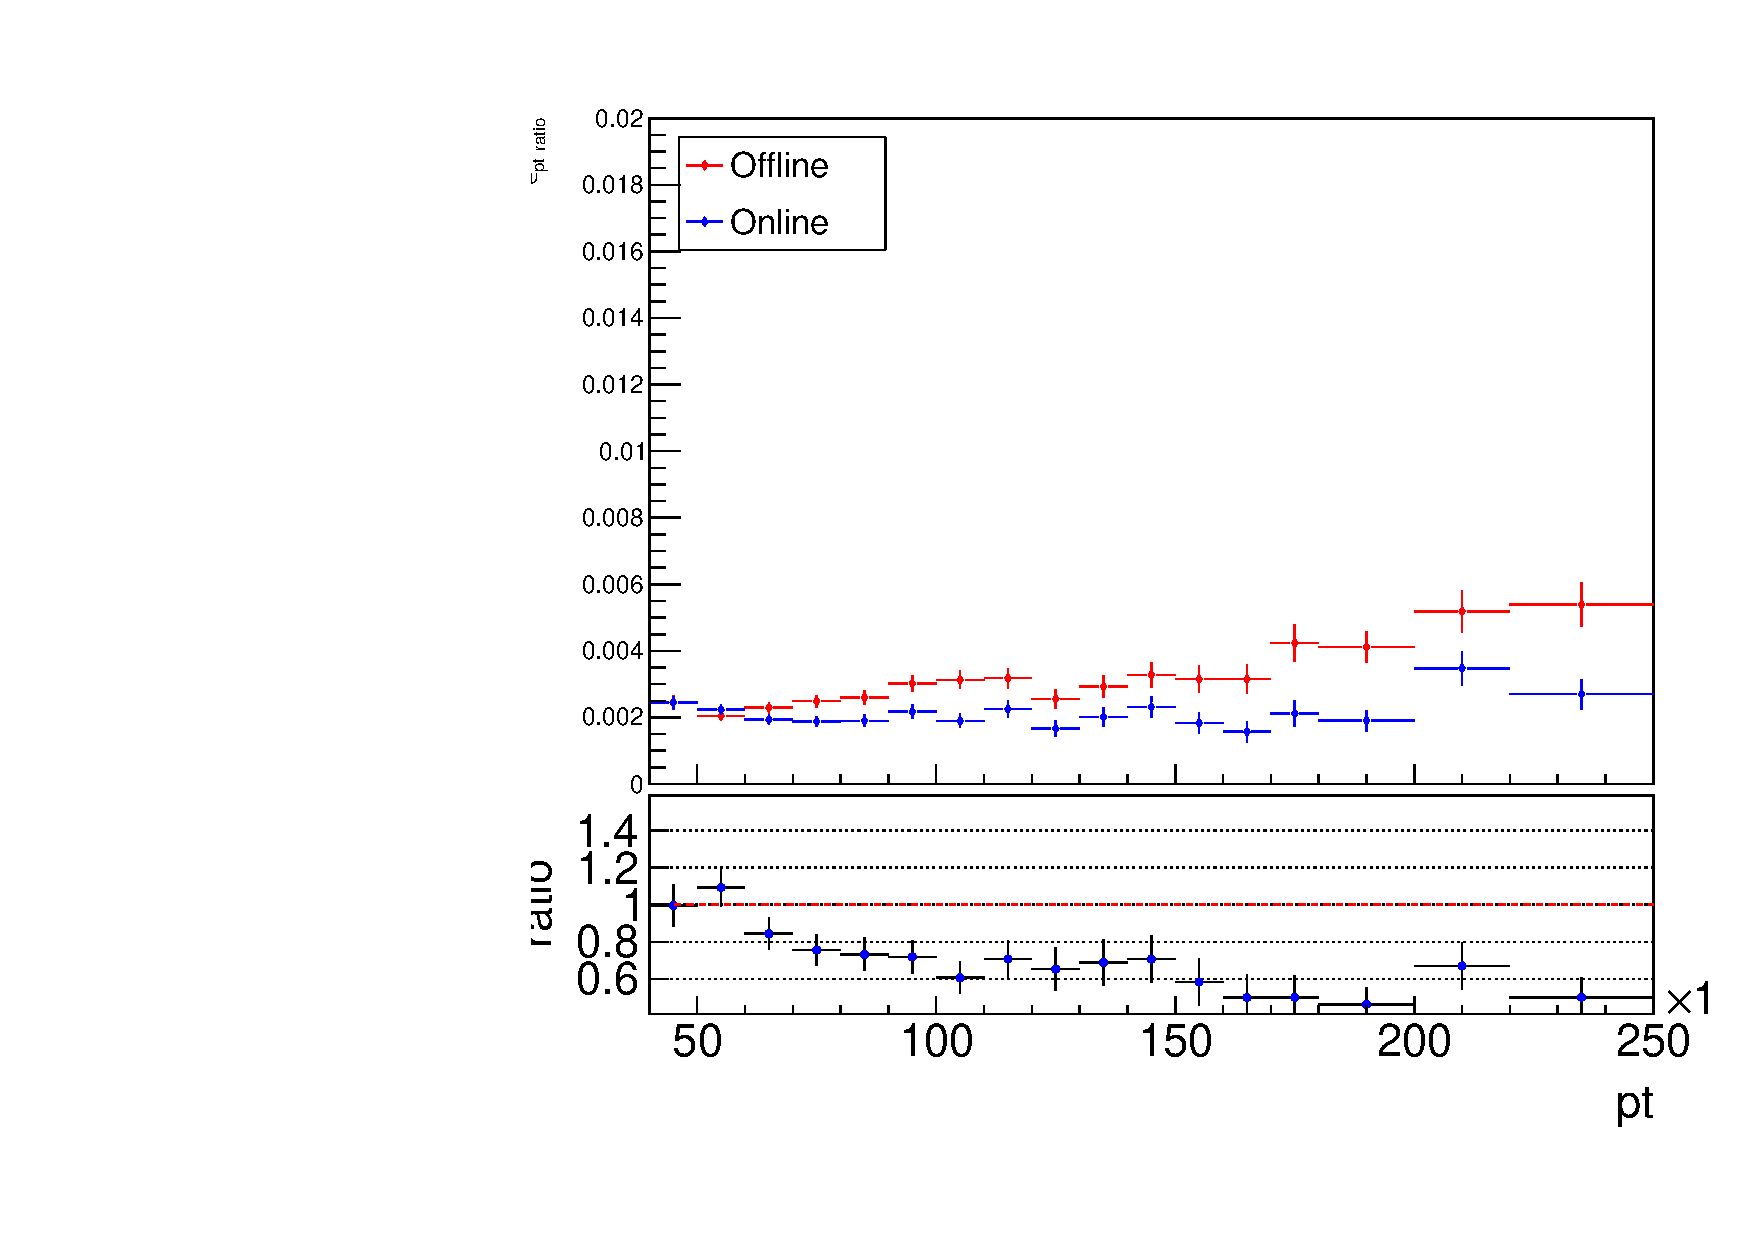
\includegraphics[width=1\linewidth]{ptLIGHTJET}

			\end{minipage}
			\quad
			\begin{minipage}[h]{0.48\linewidth}
				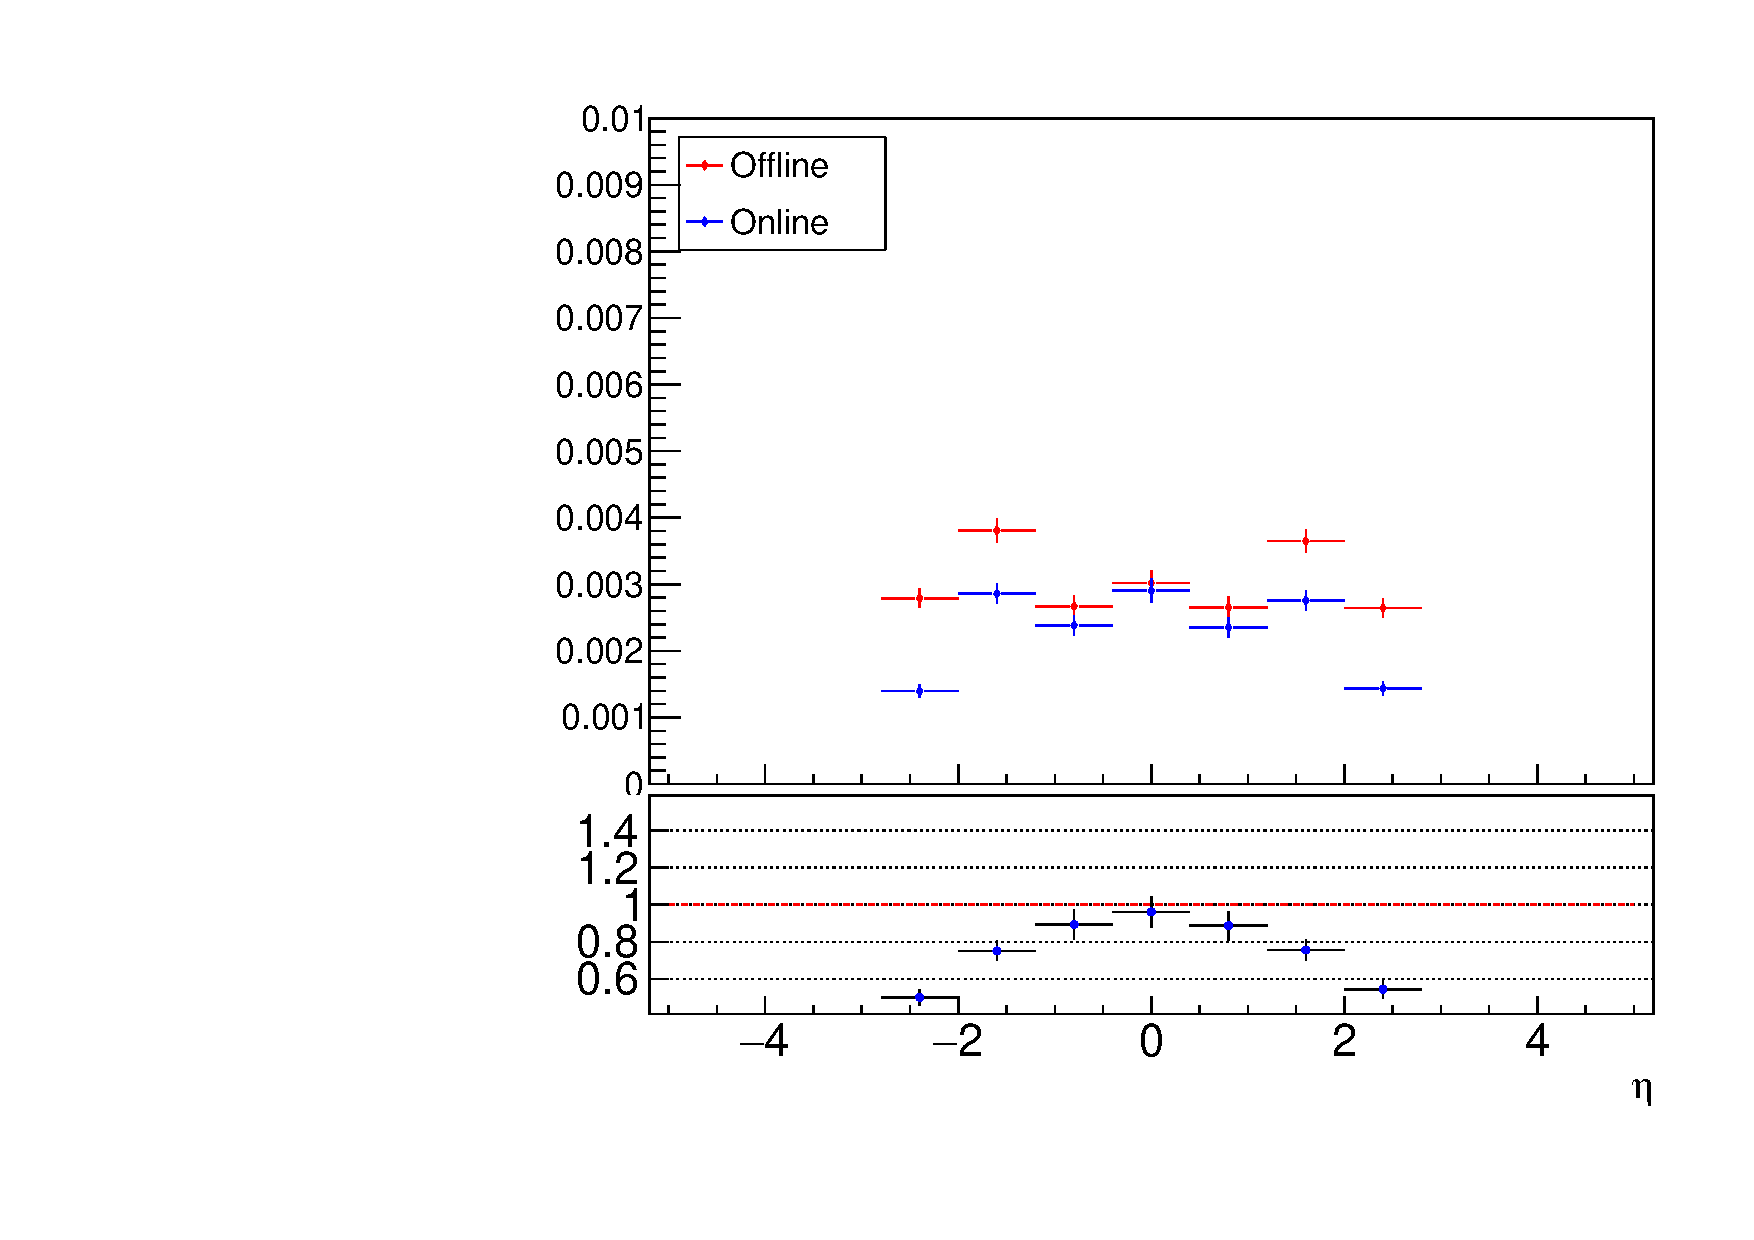
\includegraphics[width=1\linewidth]{etaLIGHTJET}
			\end{minipage}
			\caption{Mistag rate for truth light-jets in Monte-Carlo data, plotted against jet \pt (left) and $\eta$ (right). Analysis is confined to the central region of the detector where \btag\, is operational.}
			\label{fig:MC:lightjetefficiency}
		\end{figure}


	\subsection{Tag Matching}

	For each pair of jets that could be matched between online and offline, and then successfully have a \btag\, decision evaluated on the jets, the agreement of the \btag\, between the two jets was checked. These were found to match one another in $91\%$ of cases.

	\subsection{Comparison of HLT and offline tagging efficiencies}

		Primarily considering the \pt plots of efficiency, the HLT \btag\, is found to be around 5\% less efficient than the offline \btag\, for jets with \pt$>50$GeV. This is a consistent direction of efficiency shift as found when comparing the 2016 MV2c10 and 2015 MV2c20 algorithms on the training $t\bar{t}$ sample, but of a larger magnitude. The increase in the rate of \cjet\, mistagging is absolutely consistent with the refinements to the algorithm between the 2016 MV2c10 and 2015 MV2c20, with increased levels of \cjet\, rejection in the offline 2016 MV2c10, and the $\sim40$\% increase is consistent with the expected shift from the optimised algorithm \cite{btagOptimisation}.


\endinput


\graphicspath{{K/FIGS/}{.}}
\chapter{\VBFHBB\, Analysis}\label{c:K}

    After finding the base constituents of the \VBFHBB\, event at the offline and HLT levels to be similar in behaviour, the specific objects that make up a \VBFHBB\, event can be studied and compared. In this Section, the events were required to pass all cuts discussed in Section \ref{es:as}.


\section{Cutflow}
\label{k:cutflow}

    Prior to investigating the kinematic variables of the \VBFHBB\ event and the variables used for the BDT training (Appendix \ref{a:bdt}), the event cutflow for both the Monte-Carlo simulations and data should be studied to highlight any differences between the event counts. These counts are given in Table~\ref{t:cutflow}, and the ratio of the events is shown in Figures \ref{f:cutflowMC} and \ref{f:cutflowD}.

    \begin{table}[h]
        \caption[Results cutflow for the \textit{two-central} \VBFHBB\, events]{Cutflow for the \textit{two-central} \VBFHBB\, events as described in Section~\ref{es:as}. The cutflows are given for the online and offline channels in both data and Monte-Carlo.}
        \label{t:cutflow}
        \medskip
        \centering
        \begin{tabular}{c|c|c|c|c}\toprule
            Cut & MC Offline & MC Online & Data Offline & Data Online \\\midrule
            Clean Events & 6229.48 & 6229.48 & 150611000 & 150611000 \\
            Trigger & 6229.48 & 6229.48 & 6679390 &  6679390 \\
            $\geq2$ \textit{loose} \bjets & 503.552  & 467.146 & 2275760 &  2932620 \\
            $\geq2$ light-jets & 483.499  & 417.845 & 2189700 &  2671280 \\
            \textit{Tight} \bjet\, requirement & 330.962  & 288.806 & 1490320 &   1640290 \\
            Forward jet requirement & 51.843   & 40.8484 & 1186610 &  958414  \\
            \ptbb$>160$GeV & 32.7426  & 26.7038 & 309454  &  259411  \\
            \bottomrule
        \end{tabular}
    \end{table}

    \subsection{Monte-Carlo}
        \begin{figure}[h]
            \centering
            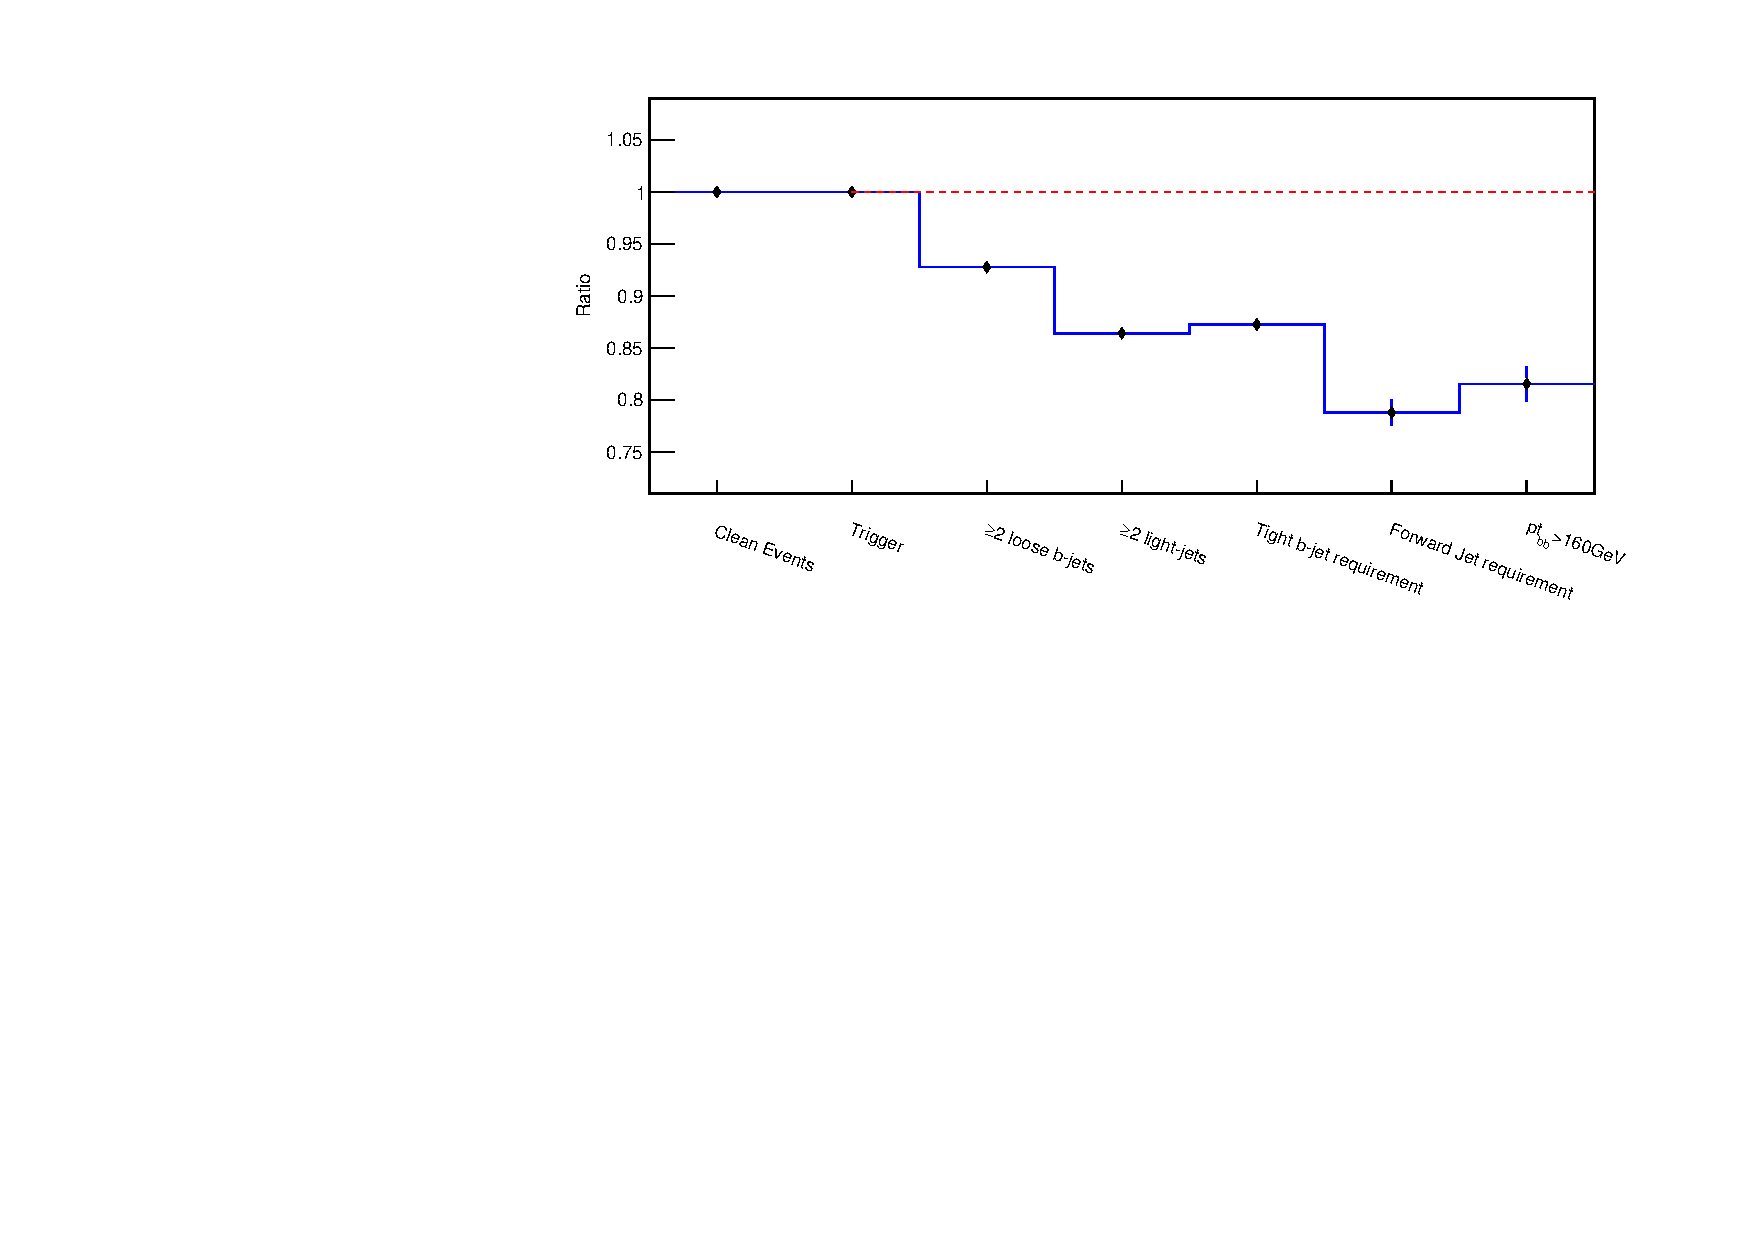
\includegraphics[width=0.75\linewidth]{MC_cutflow}
            \caption[\VBFHBB\ Cutflow ratio for Monte-Carlo simulation]{Ratio of the online event count over the offline event count for the Monte-Carlo simulations.}
            \label{f:cutflowMC}
        \end{figure}

    The online performance has fewer events than the offline for all points in the cutflow, and overall produces $\sim82\%$ of the total signal events. There are three distinct jumps in the cutflow ratio: at the cuts on the \textit{loose} \bjets, light-jets and the forward jet requirement, of $\sim7\%$ each. As shown in Figure \ref{fig:MC:bjetefficiency}, online \btag\, is $\sim93\%$ as efficient as the offline \btag\ in Monte-Carlo simulations. When considering tagging two distinct \bjets, any difference in efficiency is squared. Given the difference in tagging rates, this would result in $\sim86\%$ tagging efficiency for two \bjets\,, which is lower than shown in the cutflow. As shown for the leading \bjet\ in Section \ref{OP:leadingb}, the offline jet is typically higher in \pt than the corresponding online jet. However the difference is small, $\sim2\%$, so any effect on the cutflow should not be very pronounced.

    The $\sim7\%$ drop on the light jet requirement is unexpected, as the requirement was solely for 2 jets with \pt$>20$GeV. Given the points above with respect to the \pt difference between online and offline, this drop should not be so severe. The fact the \pt cuts on the light jets were so low also suggests an anomalous result, as such a cut should not contribute a significant reduction in either online or offline events.

    Following the drop for the light-jet cut, there is an unexpected increase in the online ratio following the \textit{tight} \btagging\, cut. As highlighted, the tagging efficiency was worse for online than offline, so any requirement for a tagged \bjet\, would be expected to produce a decrease in the online event count, relative to the offline count. Perhaps spuriously, the cutflow at this point corresponds to the $86\%$ figure expected given the relative tagging efficiency for two \bjets.

    The final drop occurs following the requirement for a high \pt forward jet. Figure \ref{fig:O:leadingnonbptslice} shows that for non-\bjets\ in the forward region of the detector, the \pt of the offline jet is consistently higher than the online $p_\text{T}$. This difference would result in a drop in the online events, with fewer jets passing the threshold \pt cut compared to the offline events.

    For the Monte-Carlo events, while the individual steps of the cutflow show some unusual results, the overall effect was an 18\% reduction in the number of events that passed the \VBFHBB\, cuts.

    \subsection{Data}
        \begin{figure}[h]
            \centering
            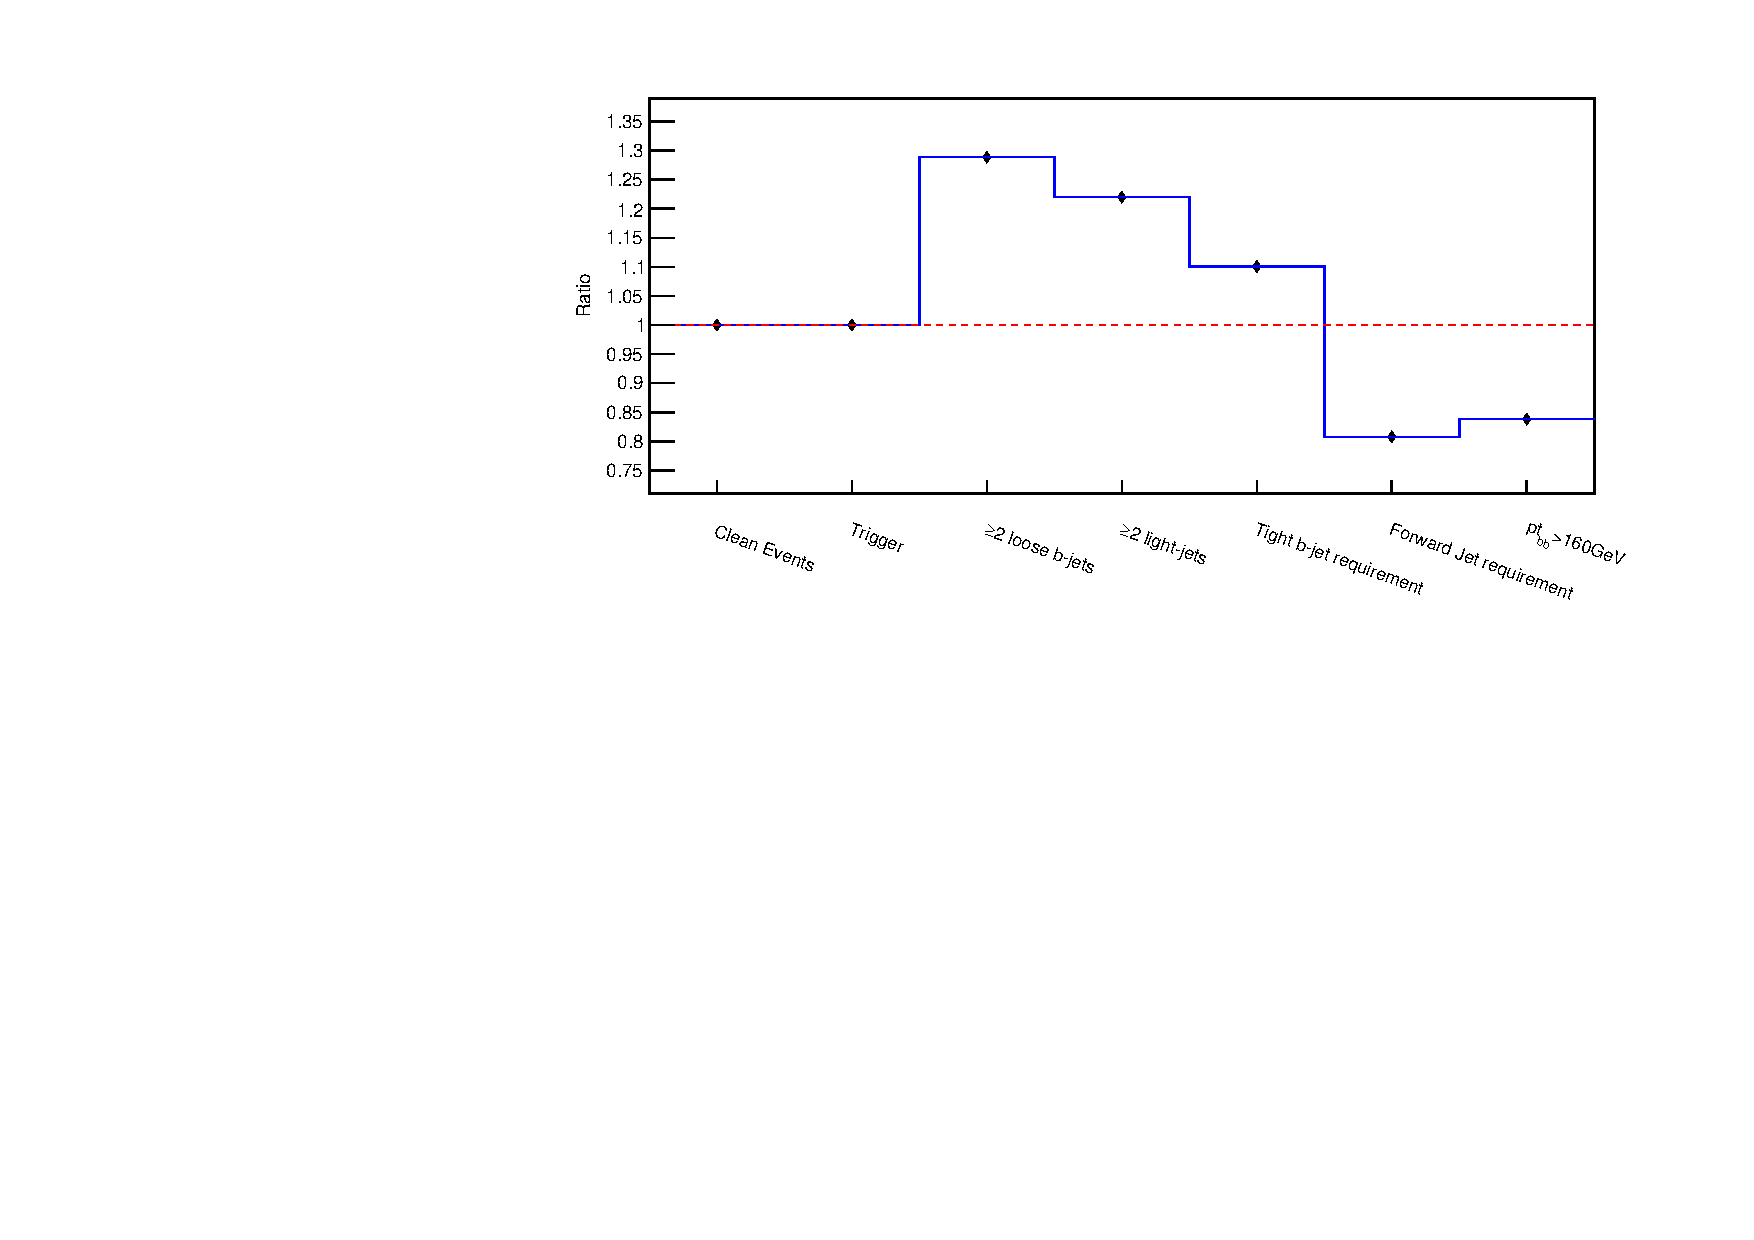
\includegraphics[width=0.75\linewidth]{D_cutflow}
            \caption[\VBFHBB\ Cutflow ratio for data]{Ratio of the online event count over the offline event count for the data.}
            \label{f:cutflowD}
        \end{figure}

    The cutflow performance in data shown in Figure \ref{f:cutflowD} does not show the online event count being consistently lower that the offline as demonstrated for the Monte-Carlo simulations in Figure \ref{f:cutflowMC}. The overall effect of the cutflow for data described by Table \ref{t:cutflow} is a reduction in online events compared to offline events of $\sim84\%$.

    The first step shows a 25\% increase in the number of events passing the loose \bjets\ cut online compared to offline. This result is not expected if the \btag\ differences between the MV2c10 and MV2c20 algorithms shown for the Monte-Carlo simulations (Figure \ref{fig:MC:bjetefficiency}) are consistent in the data. Assuming the \btag\ performs in the same way for data as for Monte-Carlo simulations, a decrease would be expected after this cut, rather than an increase.

    After this increase, there is a drop in ratio of $\sim 7\%$, which is consistent with the drop shown in the Monte-Carlo Figure \ref{f:cutflowMC}, but as discussed in the previous Section this drop is not expected from the Chapter \ref{c:OP} results regarding non-\bjet\ performance. Following this drop, there are two more drops in the ratio value, for the tight \bjet\ requirement and forward \bjet\ requirement. While these drops are expected, the magnitude of them (15\% and 30\% respectively) is much higher than could be expected.

    This sharp drop on the forward jet requirement could suggest that in the online events in the data, the jet collection is partitioned differently to the offline jet collection. If the online jet collection contained more \bjets\ proportionally to non-\bjets\ than the offline jet collection, the increase at the $\geq2$ loose \bjet\ cut could be explained by having more jet objects marked as \bjet\ candidates than the offline, which in turn, assuming there is a consistent jet population in both online and offline, would leave fewer jet candidates for the forward jet requirement. The likely source of this discrepancy arises in the process of building the jet collection discussed in Section \ref{es:jetextract}, which in future TLA applications should be formalised.

    The individual steps of the data cutflow are not in agreement with the expected comparative behaviour of the online and offline jet objects. However, the end result of the applied cuts to the data was a $16\%$ reduction in the number of online events compared to offline.

    \subsection{Summary of Cutflow Comparison for the Online and Offline \VBFHBB\ events}

    The final reduction in online event count relative to the offline event count for the Monte-Carlo simulations was $\sim82\%$ of the offline event count, and $\sim84\%$  for the data. The results from individual steps in the cutflow are not supported by the results of Chapter \ref{c:OP}, but these overall results, which are broadly consistent for both data and Monte-Carlo, are supported by the expected decrease in efficiency as a result of the diffent \btag\ algorithms. Looking only at the overall reduction at the final states suggests that future analyses may be able to apply TLA to the \VBFHBB\ channel to increase the final event yield.

    With an average $\sim83\%$ reduction in event rate for the channel, usage of TLA at a rate of $2$kHz as described in Ref. \cite{tla} and Section \ref{t:tla}, would result in an increase in output events of $\sim66\%$ compared to a standard offline analysis.

    This value is an estimate, there is additional computational cost involved with storing and computing the quantities required for TLA \VBFHBB\ analysis, such as the increased event size mentioned in Section \ref{obp:beff} as a result of storing the \btag\ training quantities. A rate analysis, to ensure the TLA can be applied in the \VBFHBB\ channel without decreasing the rate increase down to the point the final TLA event count is no longer an improvement, is a necessary step before approving TLA, but is beyond the scope of this dissertation.

\newpage
\section{Specific Jet Feature Distributions}
\label{k:jets}

    While the previous chapter showed that the \bjets\ and non-\bjets\ had slight differences that could be rectified for future analyses, the behaviour of those jets is sufficiently similar that plots of the kinematic quantities of the \VBFHBB\ jets can be made.

    \begin{table}[h]
        \caption[Signal/Background definition \mbb values]{\mbb bins defining an event as signal or background, along with the data source for the quantities.}
        \label{t:signalback}
        \medskip
        \centering
        \begin{tabular}{ccc}\toprule
            Designation & \mbb range / GeV & Sample \\\midrule
            Background (Lower) & \mbb<$100$ & Data \\
            Signal & $100<$\mbb$<140$ & Monte-Carlo \\
            Background (Upper) &  $140<$\mbb & Data \\
            \bottomrule
        \end{tabular}
    \end{table}

    These plots were presented in signal and background regions, as defined by the \mbb value as shown in Table \ref{t:signalback}. The signal was plotted only using the Monte-Carlo simulation while the background regions were taken from data events. The kinematic quantities for leading \bjet\ and leading non-\bjet\ of the \VBFHBB\ event are plotted for both the online and offline objects. The \pt distributions are shown in Figures \ref{f:ptb1} and \ref{f:ptj1} respectively, while the pseudorapidity plots are shown in Figure \ref{f:etab1} and \ref{f:etaj1}.

        \begin{figure}[h]
            \centering

            \begin{minipage}[h]{0.48\linewidth}
                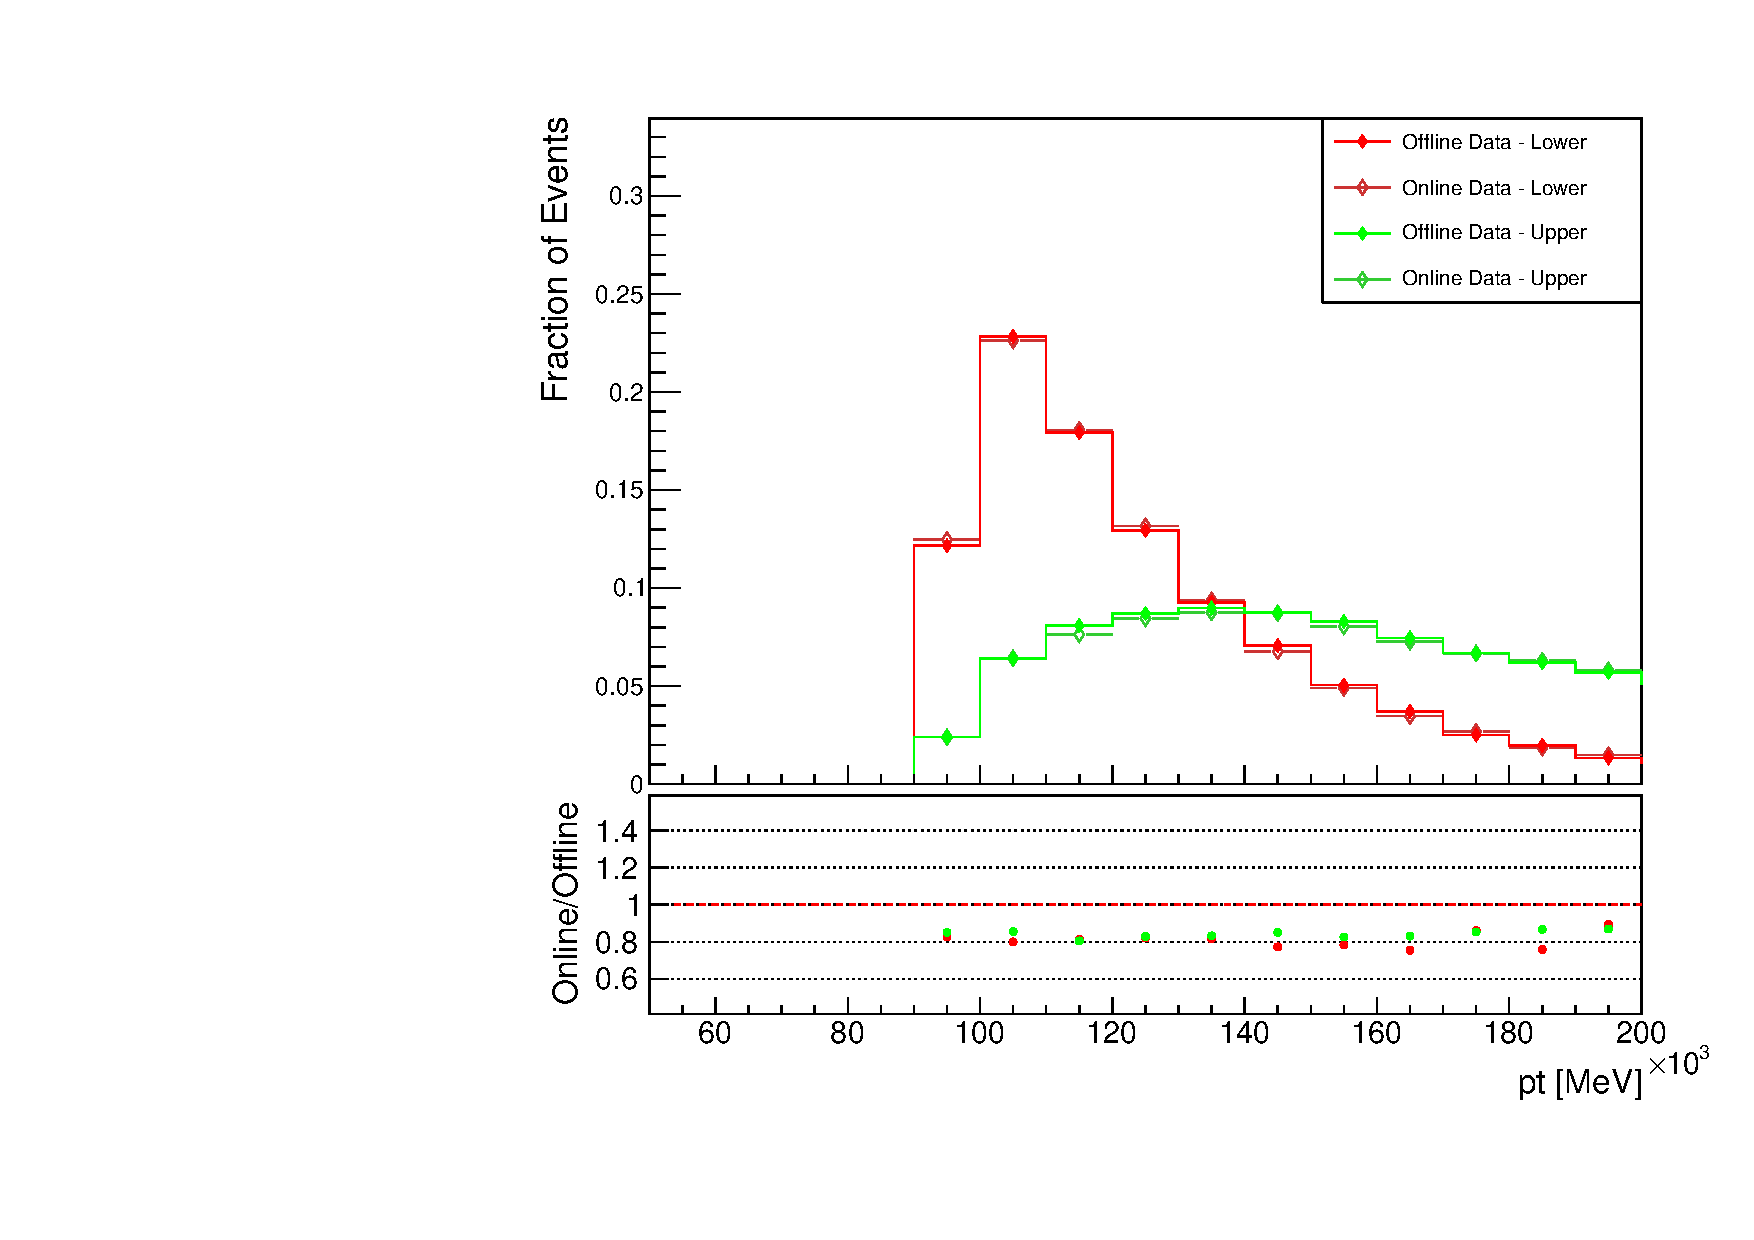
\includegraphics[width=1\linewidth]{pt_bJet1_data_}
            \end{minipage}
            \quad
            \begin{minipage}[h]{0.48\linewidth}
                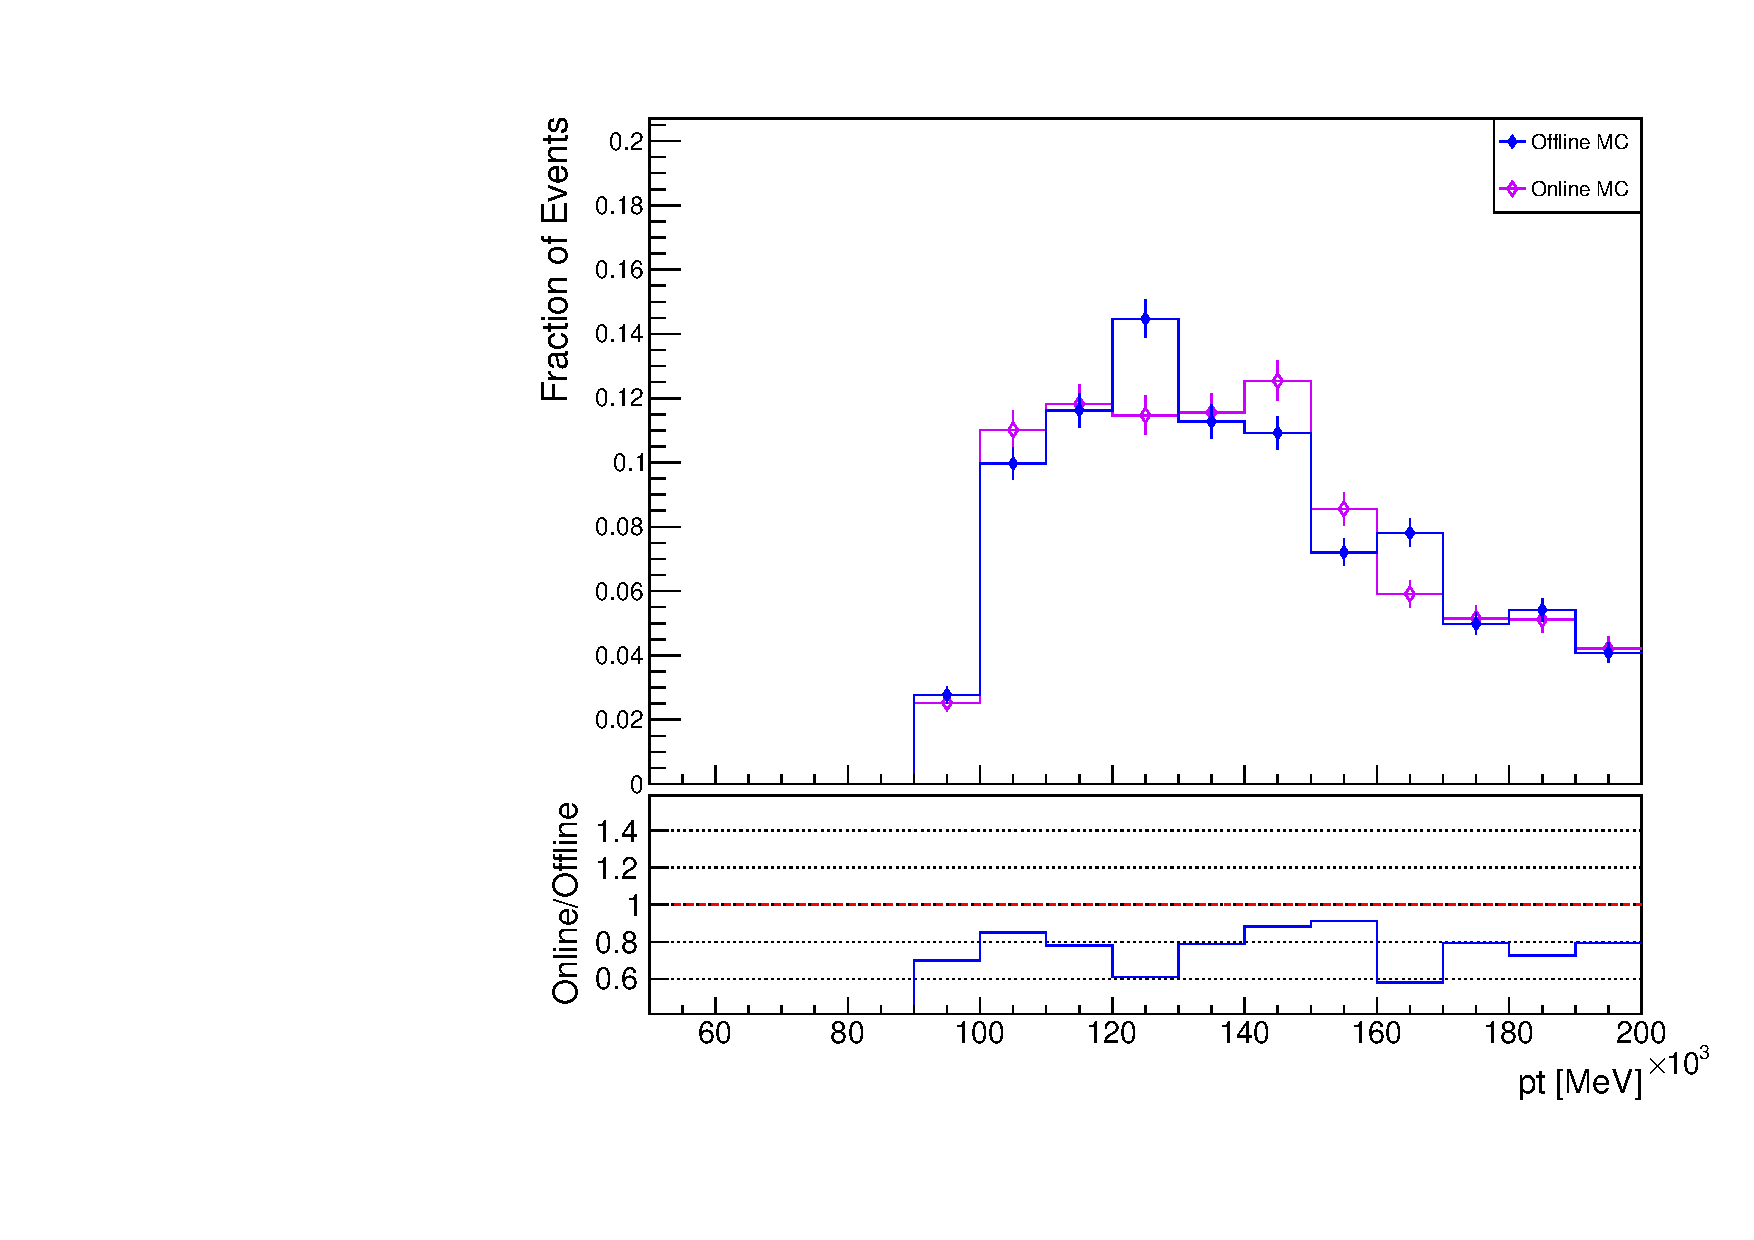
\includegraphics[width=1\linewidth]{pt_bJet1_mc_}
            \end{minipage}
            \caption[\pt distribution of the leading \bjet\ of the \VBFHBB\ event]{\pt distribution of the leading \bjet\ of the \VBFHBB\ event, plotted for both the backgroud data regions in the left panel and Monte-Carlo signal events in the right panel.}
            \label{f:ptb1}
        \end{figure}

        \begin{figure}[h]
            \centering

            \begin{minipage}[h]{0.48\linewidth}
                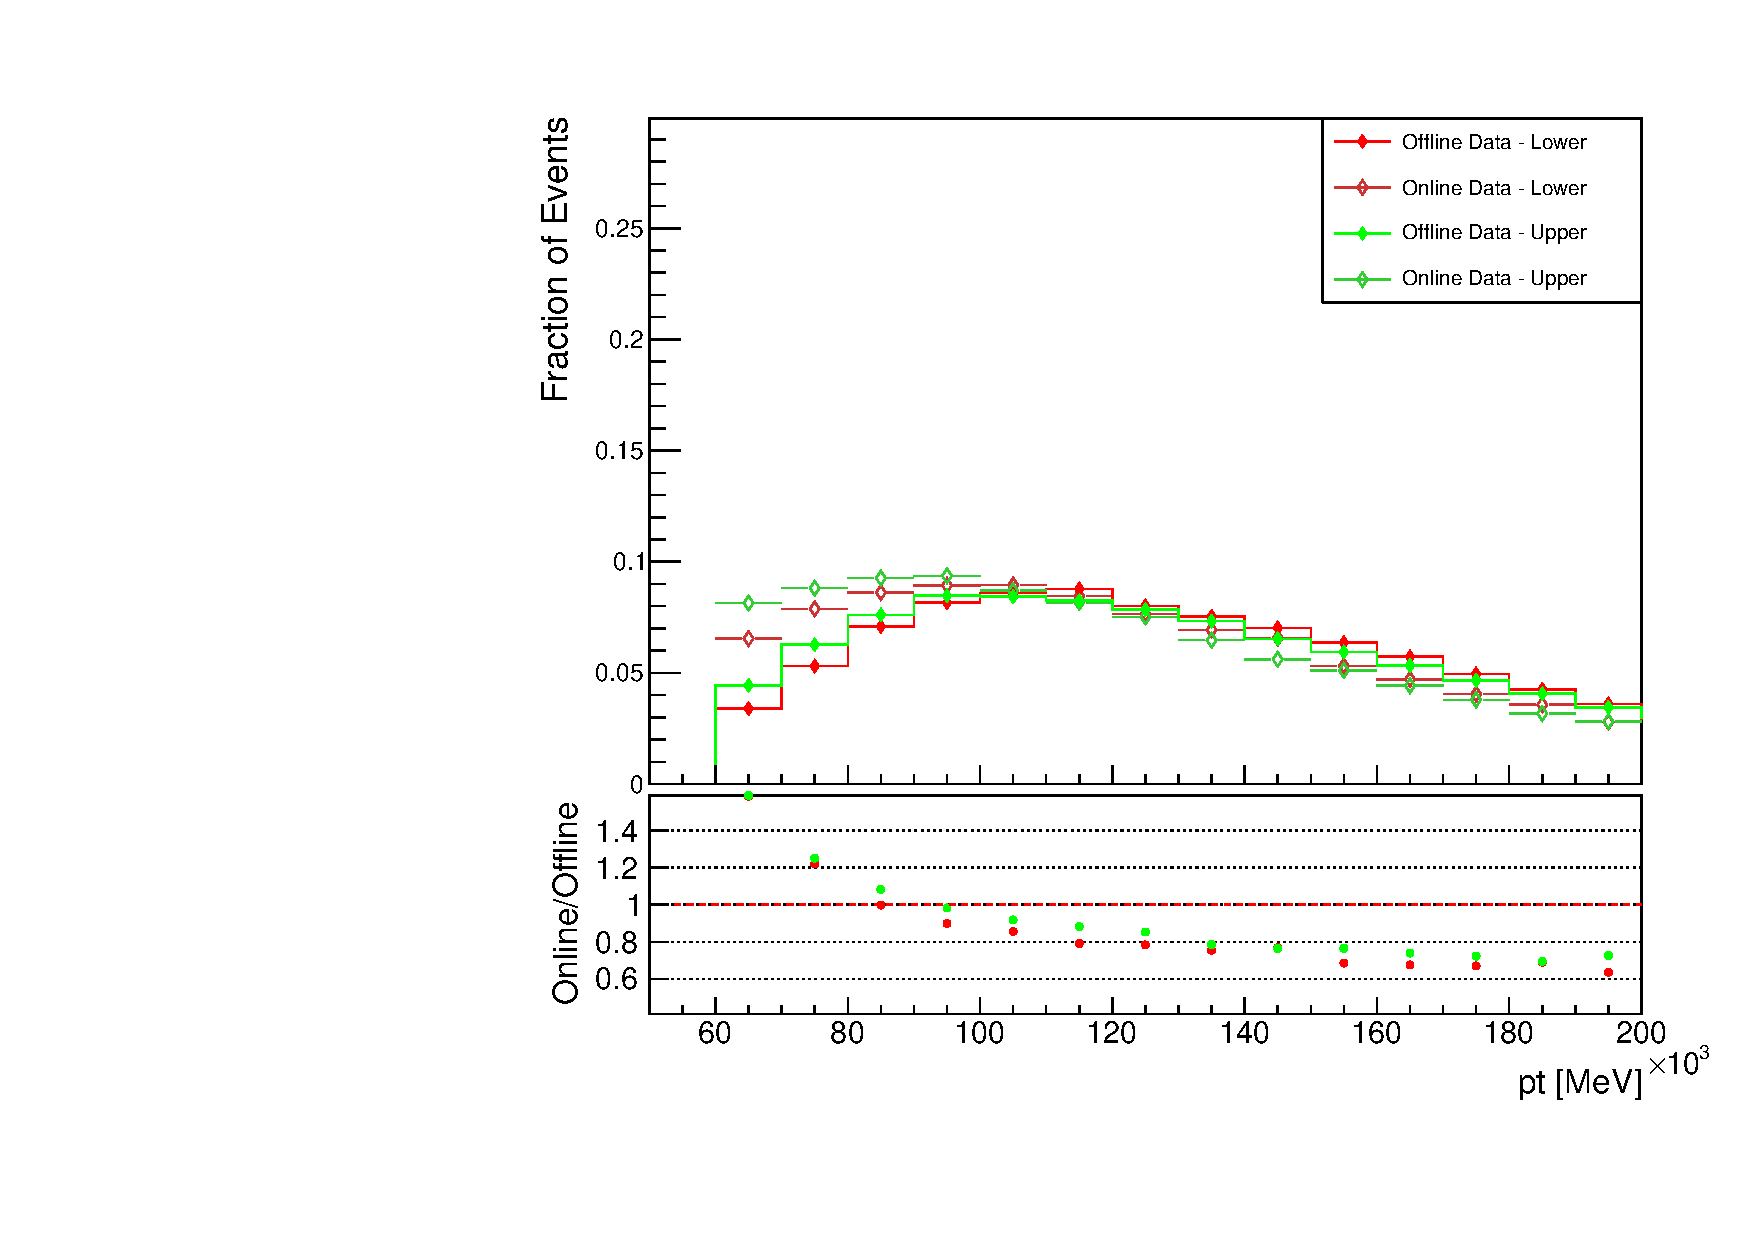
\includegraphics[width=1\linewidth]{pt_lJet1_data_}
            \end{minipage}
            \quad
            \begin{minipage}[h]{0.48\linewidth}
                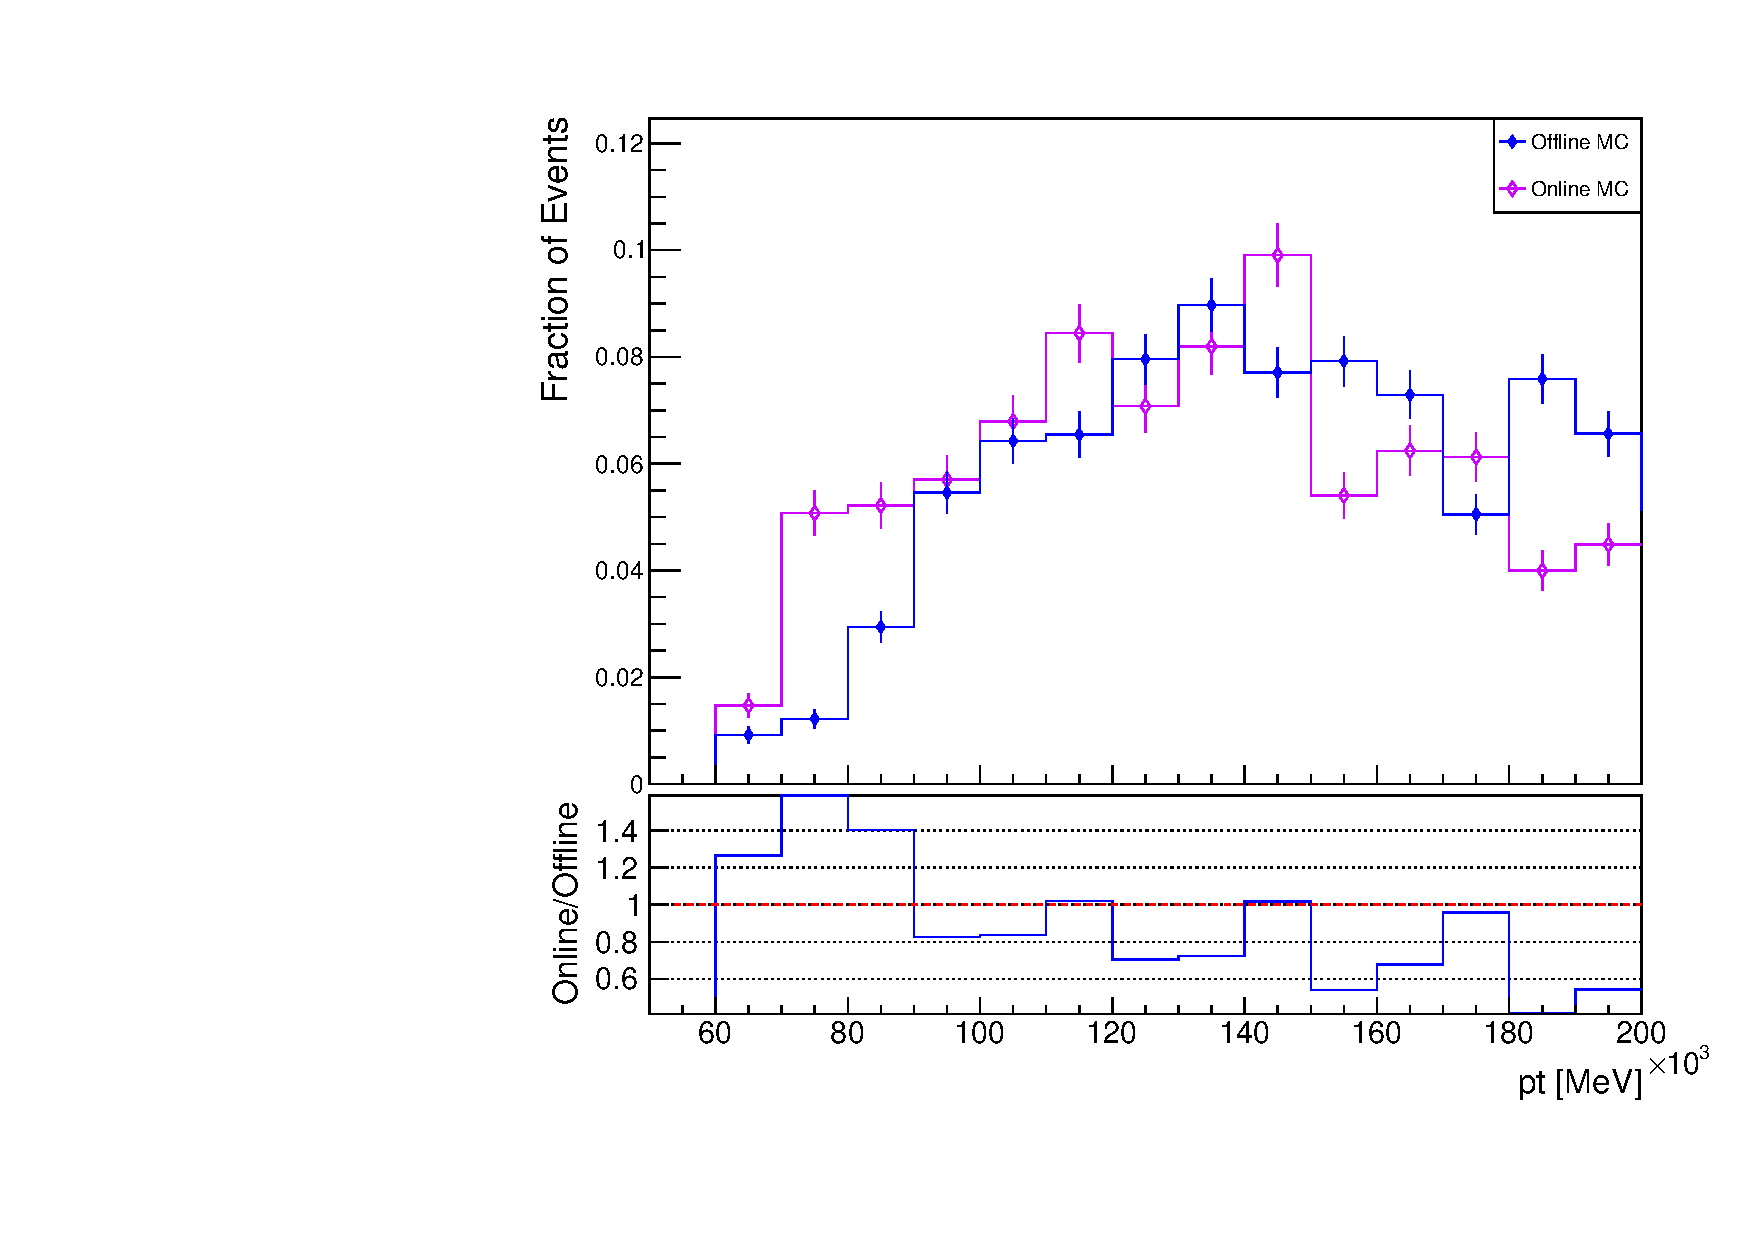
\includegraphics[width=1\linewidth]{pt_lJet1_mc_}
            \end{minipage}
            \caption[\pt distribution of the leading non-\bjet\ of the \VBFHBB\ event]{\pt distribution of the leading non-\bjet\ of the \VBFHBB\ event, plotted for both the backgroud data regions in the left panel and Monte-Carlo signal events in the right panel.}
            \label{f:ptj1}
        \end{figure}

    The distribution of the \pt values for the leading \bjet\ shown in Figure \ref{f:ptb1} peaks at a higher value for the upper background region than the lower background region. This is a result of the \mbb sculpting the background distributions, as higher \mbb values will correlate with higher \bjet\ \pt values. For the background \pt plot of the leading non-\bjet, this sculpting is not seen as the \pt of the forward jet is not directly linked to the \mbb of the event. For both the leading \bjet\ and the leading non-\bjet\, the online and offline distributions are similarly shaped for each of the defined \mbb regions.

    For the leading \bjet, the ratio of the online to the offline events shown in Figure \ref{f:ptb1} is flat in both the upper and lower background regions, and has a value of $\sim0.8$. This value is consistent with the expected decrease in the online event count shown in Figure \ref{f:cutflowD}. The Monte-Carlo signal plot shown in Figure \ref{f:ptb1}, the line is insufficiently clear to make a firm statement but the ratio values are distributed around $0.8$. For the leading non-\bjet, the behaviour of the online/offline ratio is more complex, as shown by the distinct curve in the left panel of Figure \ref{f:ptj1}. The online jets show a bias towards low \pt compared to the offline jets in both the upper and lower background regions, along with in the signal region. The relative ratio of the online and offline jets is affected by this, flattening out at a lower value of $\sim0.7$ than the expected $0.8$ in both the background regions. This bias towards lower \pt events was seen in Figure \ref{fig:O:leadingnonbpt} in the previous chapter showing the \dptpt distribution for the leading non-\bjet. Figure \ref{fig:O:leadingnonbpt} showed a large number of data jets with offline $50<$ \pt$90$GeV which had a \dptpt value between 0.1 and 0.2, indicating that for this region the offline \pt was significantly larger than the online. This observation is consistent with the left panel of Figure \ref{f:ptj1}, as it suggests there will more online jets with $50<$ \pt$<80$GeV than offline jets in the data, accounting for the shift in the distribution peaks. For the signal plot, Figure \ref{fig:O:leadingnonbpt} did not show such a pronounced discrepancy for the Monte-Carlo jets, only a slight increase of \dptpt values around 0.1 for this low \pt region, so such a shift is not absolutely expected for the signal region. In addition, as for the leading \bjet, a clear statement on the ratio of the Monte-Carlo events cannot be made, but the curve broadly follows the background ratios.

    While there are differences between the signal and background regions and the small effects at low \pt in the leading non-\bjets, for the complete \pt distributions of leading \bjet\ and most of the distribution for the leading non-\bjet\, the offline jets performed the same as the online jets. This suggests that the online jet objects could be used in a TLA without any major effects on the outcome.

    The plots for the same leading jet objects against $\eta$ show the expected features for \VBFHBB\ jets. Figure \ref{f:etab1} shows the pseudorapidity ranges for the \bjet\ confined to the central region of the detector where \btag\ is operational. The $\eta$ plot for the leading non-\bjet\ displays spikes of events with $|\eta|\sim3$, which is expected given the requirements for a forward jet passing a \pt cut covered in Section \ref{es:as}. These features are present in both the signal and background regions.

    \begin{figure}[h]
        \centering

        \begin{minipage}[h]{0.48\linewidth}
            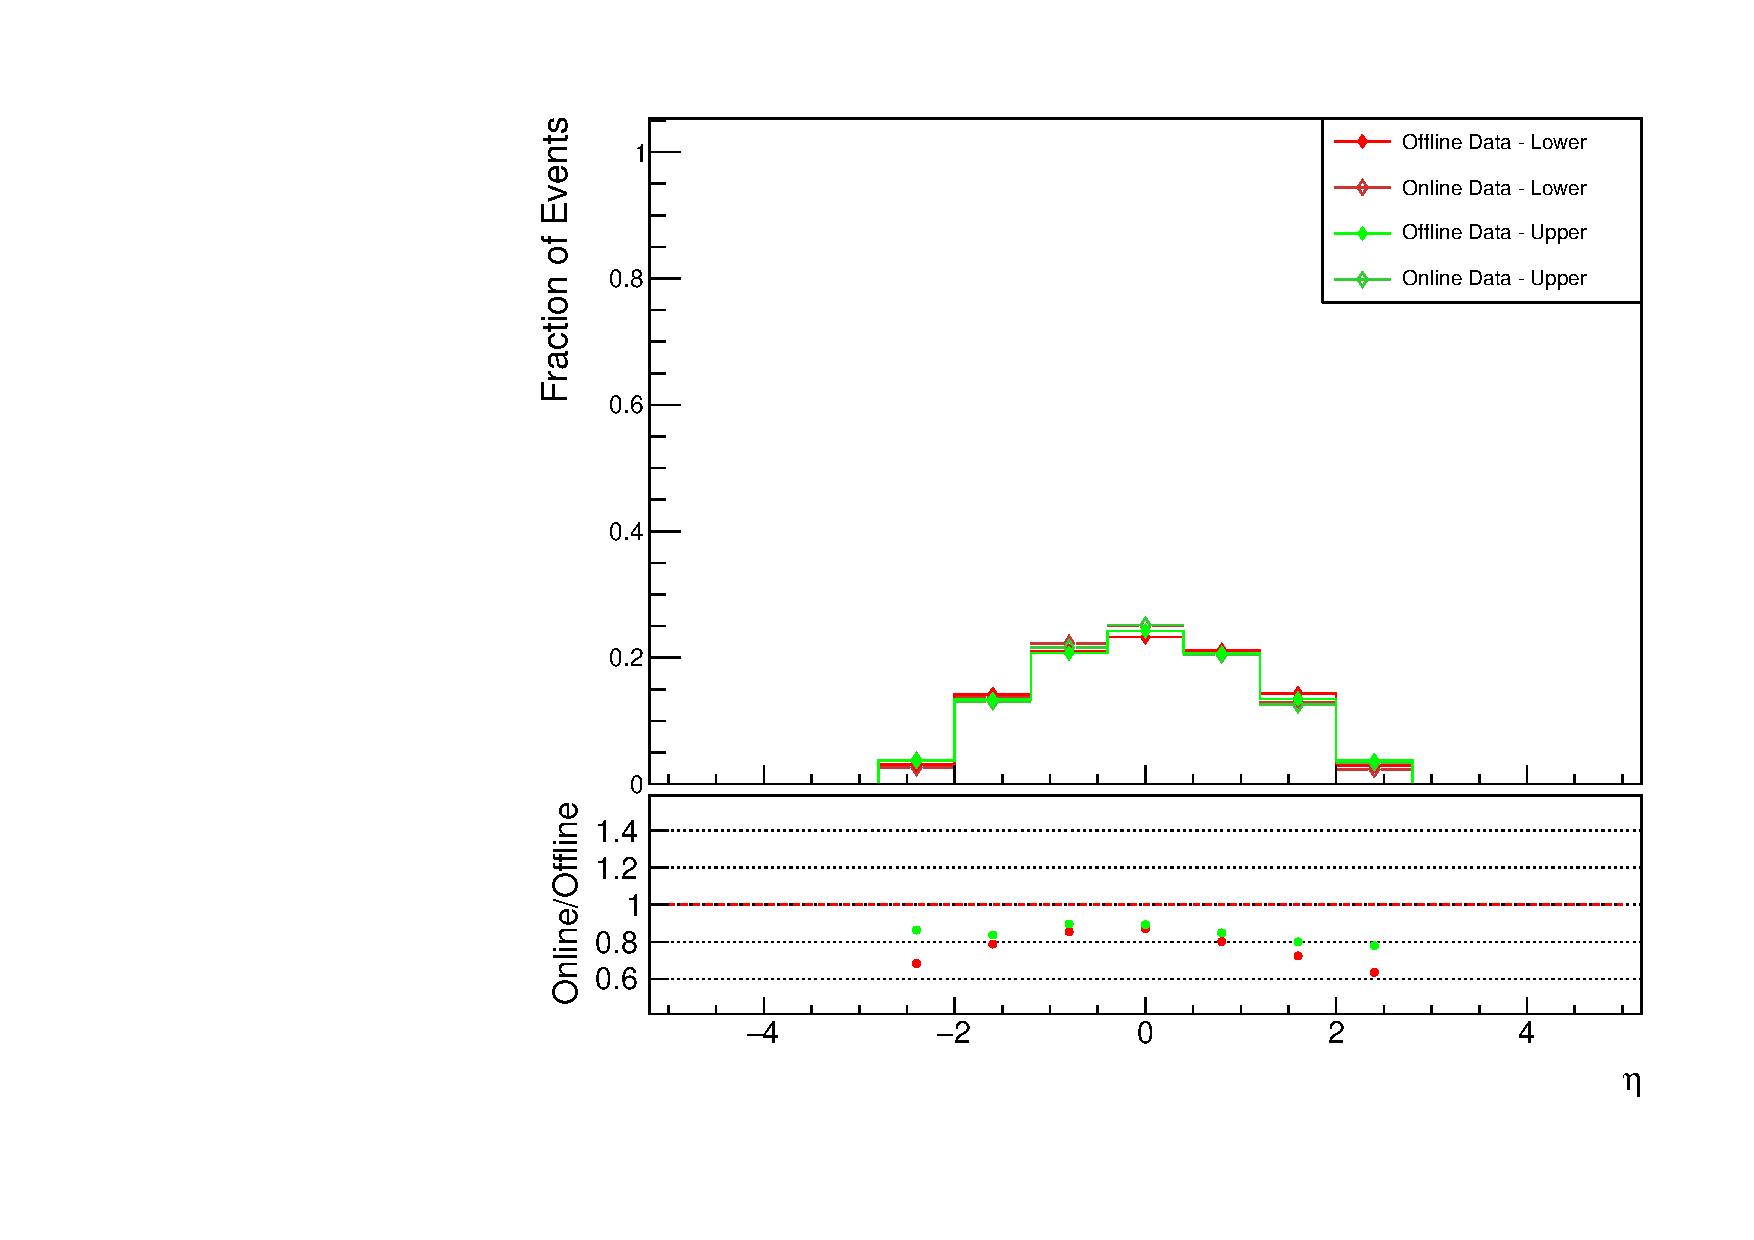
\includegraphics[width=1\linewidth]{eta_bJet1_data_}
        \end{minipage}
        \quad
        \begin{minipage}[h]{0.48\linewidth}
            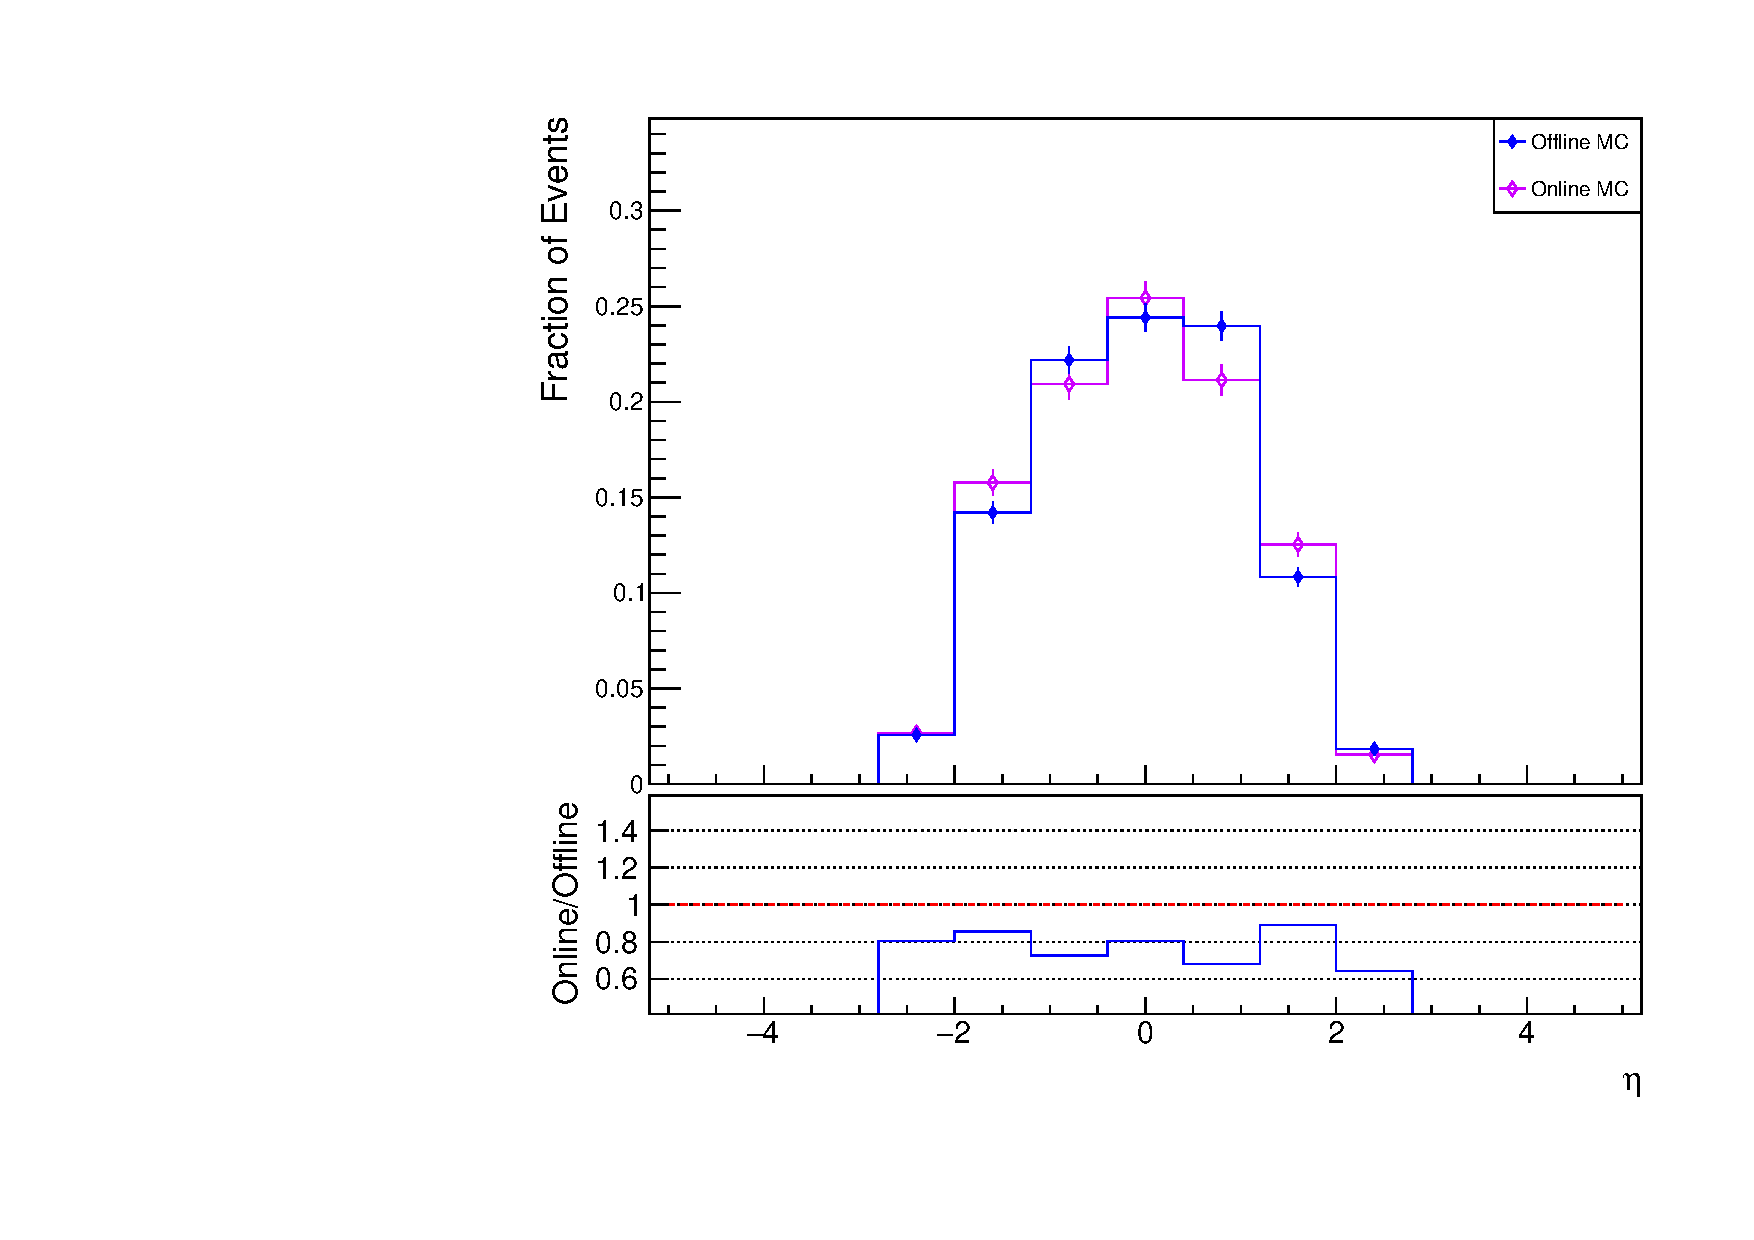
\includegraphics[width=1\linewidth]{eta_bJet1_mc_}
        \end{minipage}
        \caption[$\eta$ distribution of the leading \bjet\ of the \VBFHBB\ event]{$\eta$ distribution of the leading \bjet\ of the \VBFHBB\ event, plotted for both the background data regions in the left panel and Monte-Carlo signal events in the right panel.}
        \label{f:etab1}
    \end{figure}

    \begin{figure}[h]
        \centering
        \begin{minipage}[h]{0.48\linewidth}
            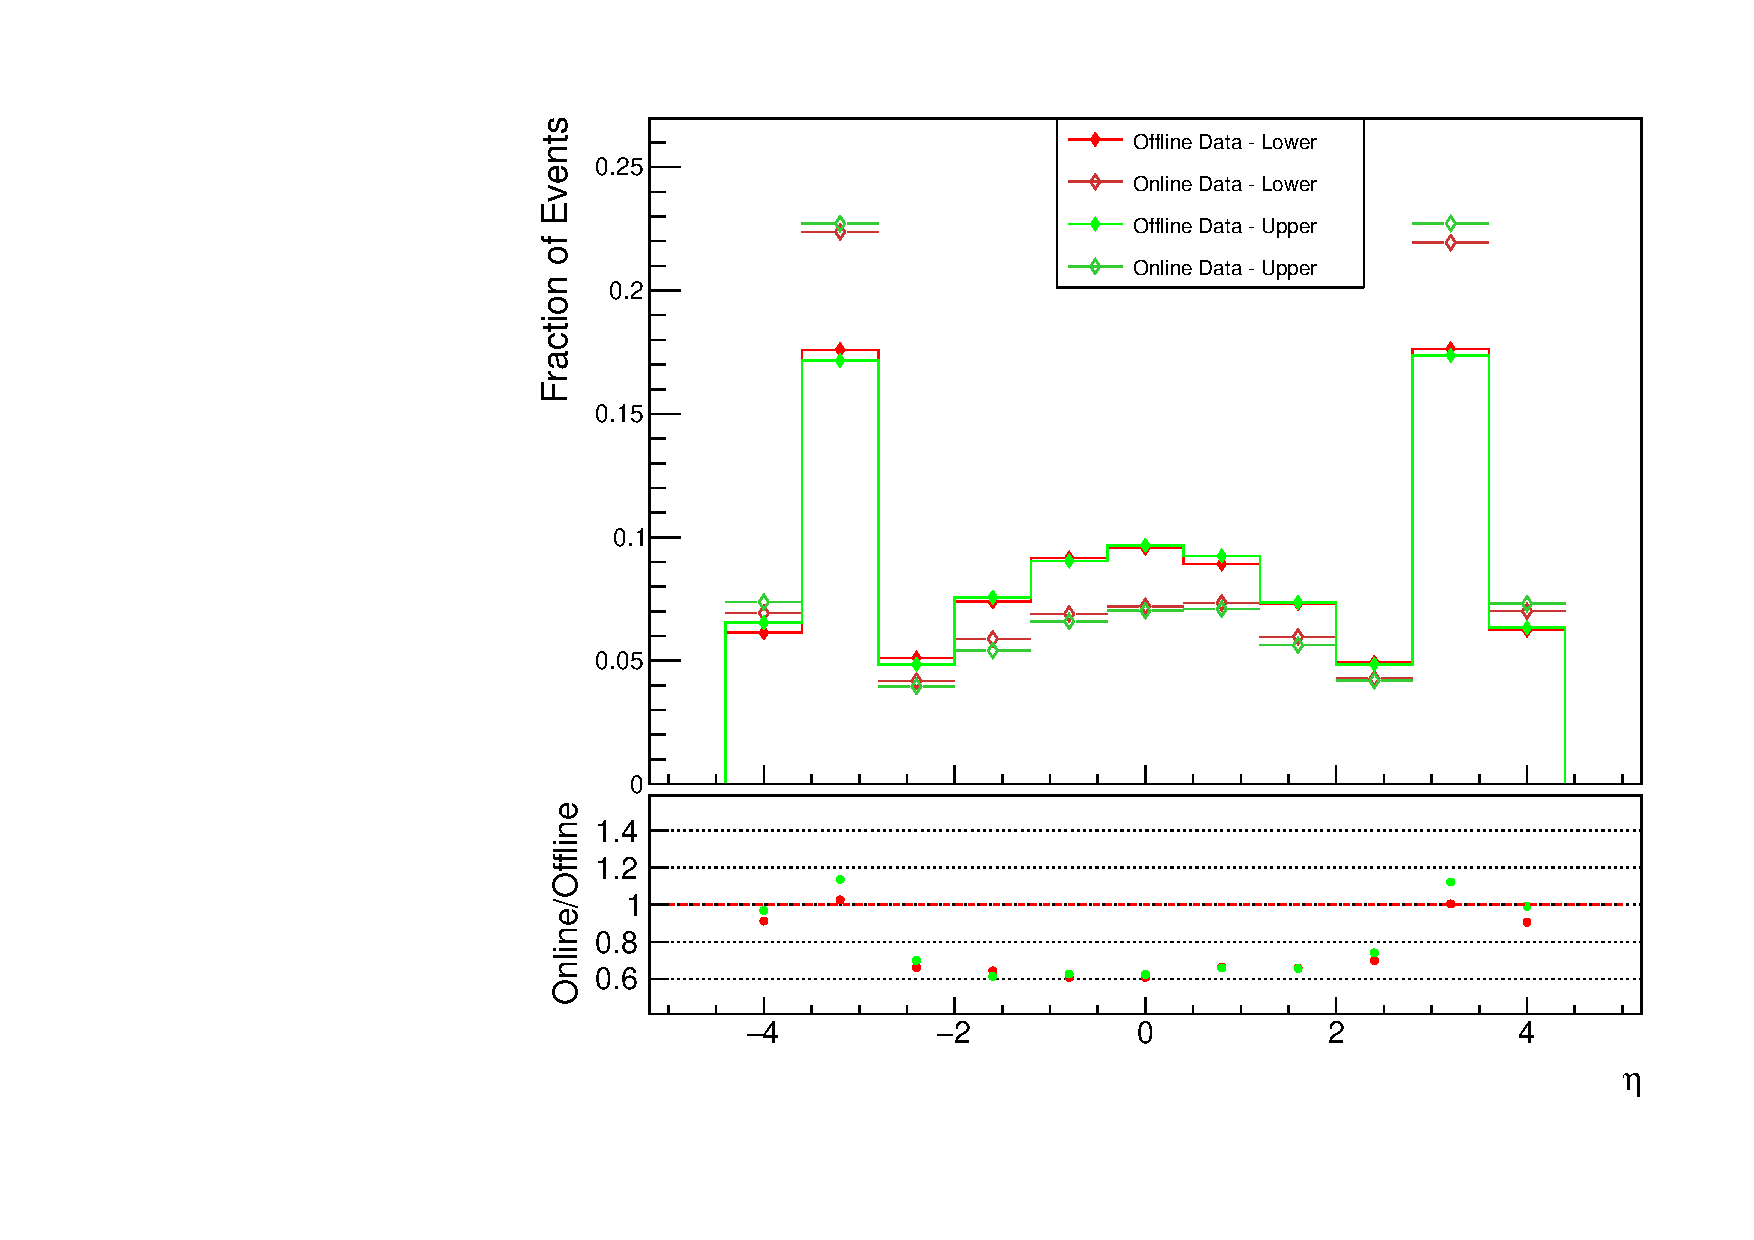
\includegraphics[width=1\linewidth]{eta_lJet1_data_}
        \end{minipage}
        \quad
        \begin{minipage}[h]{0.48\linewidth}
            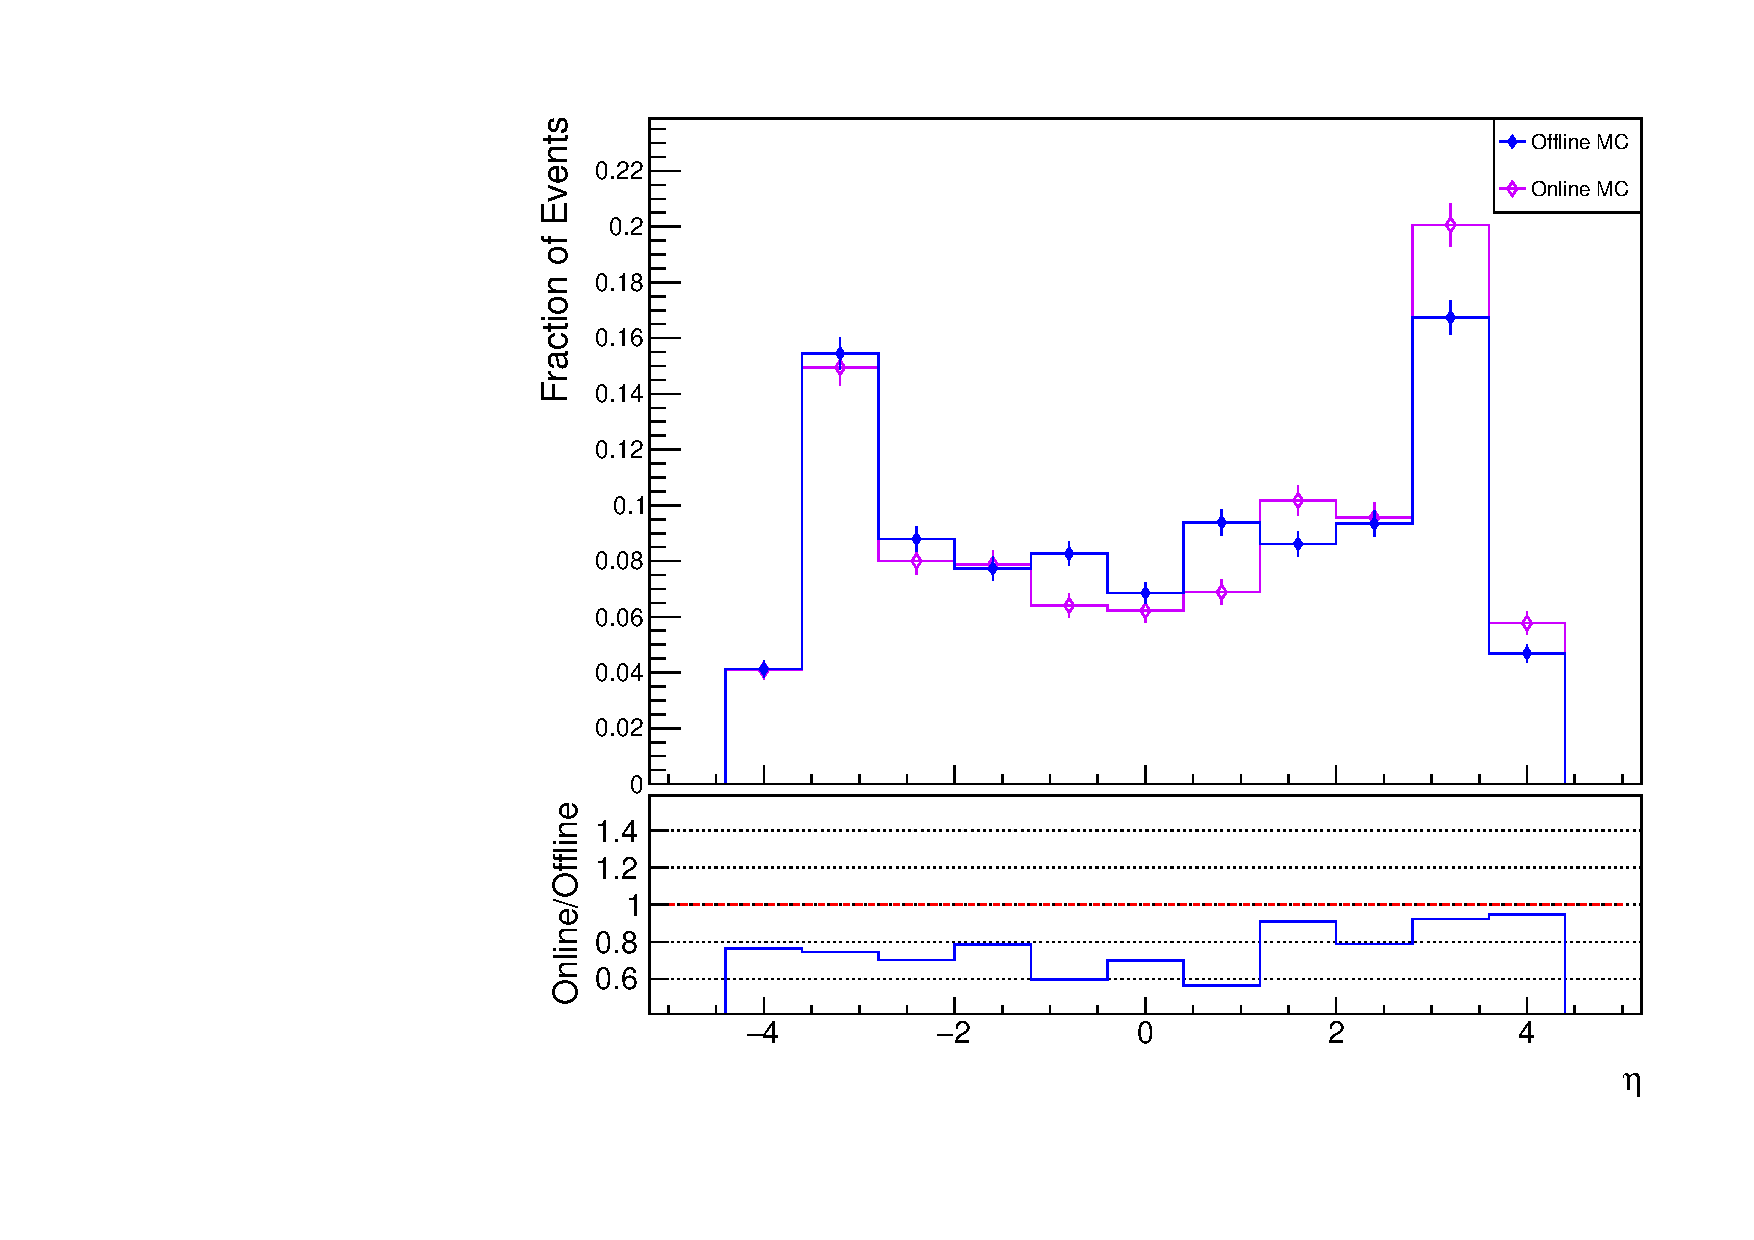
\includegraphics[width=1\linewidth]{eta_lJet1_mc_}
        \end{minipage}
        \caption[$\eta$ distribution of the leading non-\bjet\ of the \VBFHBB\ event]{$\eta$ distribution of the leading non-\bjet\ of the \VBFHBB\ event, plotted for both the background data regions in the left panel and Monte-Carlo signal events in the right panel.}
        \label{f:etaj1}
    \end{figure}

    The relative performance of online to offline shows some slight differences with respect to $\eta$. For the leading \bjet\ there is a noticeable peak in the ratio at $\eta=0$ for the lower signal region shown in Figure \ref{f:etab1}, however the upper signal region shows moderately consistent distribution around the expected $0.8$ value. The signal $\eta$ online/offline ratio has a larger degree of variation but is consistently around $\sim0.8$. For the leading non-\bjet\ shown in Figure \ref{f:etaj1} the ratio for the upper and lower background sectors is lower than expected in the central region of the detector, but increases in the forward regions. For the signal sector, the distribution suggests a slight increase of the ratio at the outer $\eta$ regions, but the difference is less pronounced than in the background regions.

    Overall, the behaviour of the leading jets of the \VBFHBB\ event was fairly consistent for online and offline in most phase space regions. The plots showed the distribution features expected for the variables and the differences associated with the \mbb bins, along with showing agreement with the reduction in event number for online events. The discrepancy in online behaviour relative to the offline for the low \pt leading non-\bjets\ can be explained by the observed differences in the non-\bjet\ objects explored in the previous Chapter, however the cause of the improved relative performance of the online objects in the forward regions for the leading non-\bjet\ are unknown. The upper background sector frequently had a higher ratio than the lower background sector, as shown across the entire \pt range in Figures \ref{f:ptb1} and \ref{f:ptj1}. These observations suggest a TLA using these objects would show little change in the overall behaviour, and if the calibration steps suggested in Section \ref{obp:jetsum} were applied, the differences in the online and offline behaviour may be removed.


\section{Kinematic quantities of the \VBFHBB\ event}

	Along with studying the kinematic quantities associated with single \VBFHBB\ jets, the kinematic properties of the jet pairs were compared for online and offline. For the non-\bjet\ pair, \ptjj and \mjj are plotted in Figures \ref{f:ptjj} and \ref{f:mjj}. Both of these variables are also used as training variables to the BDT used to refine the produced results (Appendix \ref{a:bdt}). Figure \ref{f:ptbb} shows the \ptbb distribution and Figure \ref{f:mbb} shows the \mbb distribution.

        \begin{figure}[h]
            \centering
            \begin{minipage}[h]{0.48\linewidth}
                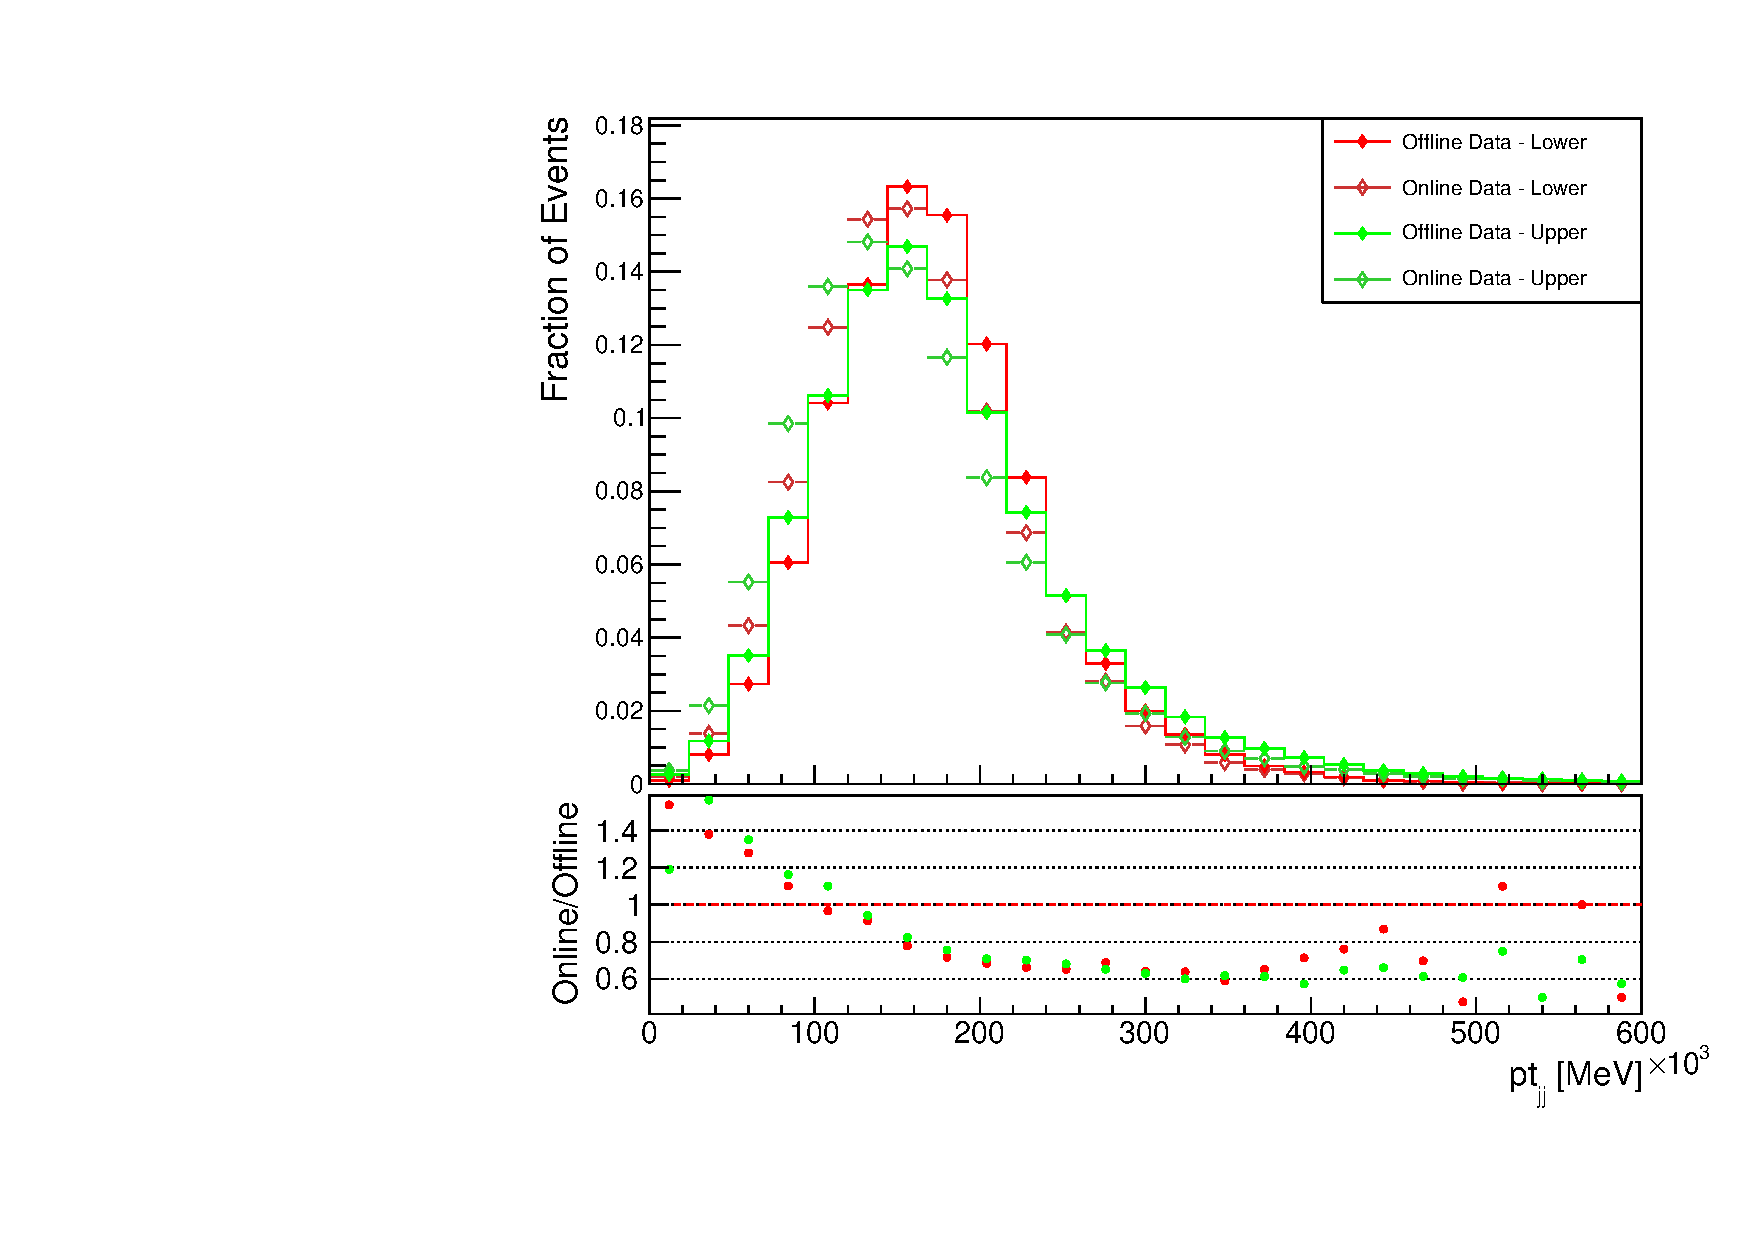
\includegraphics[width=1\linewidth]{ptjj_data_}
            \end{minipage}
            \quad
            \begin{minipage}[h]{0.48\linewidth}
                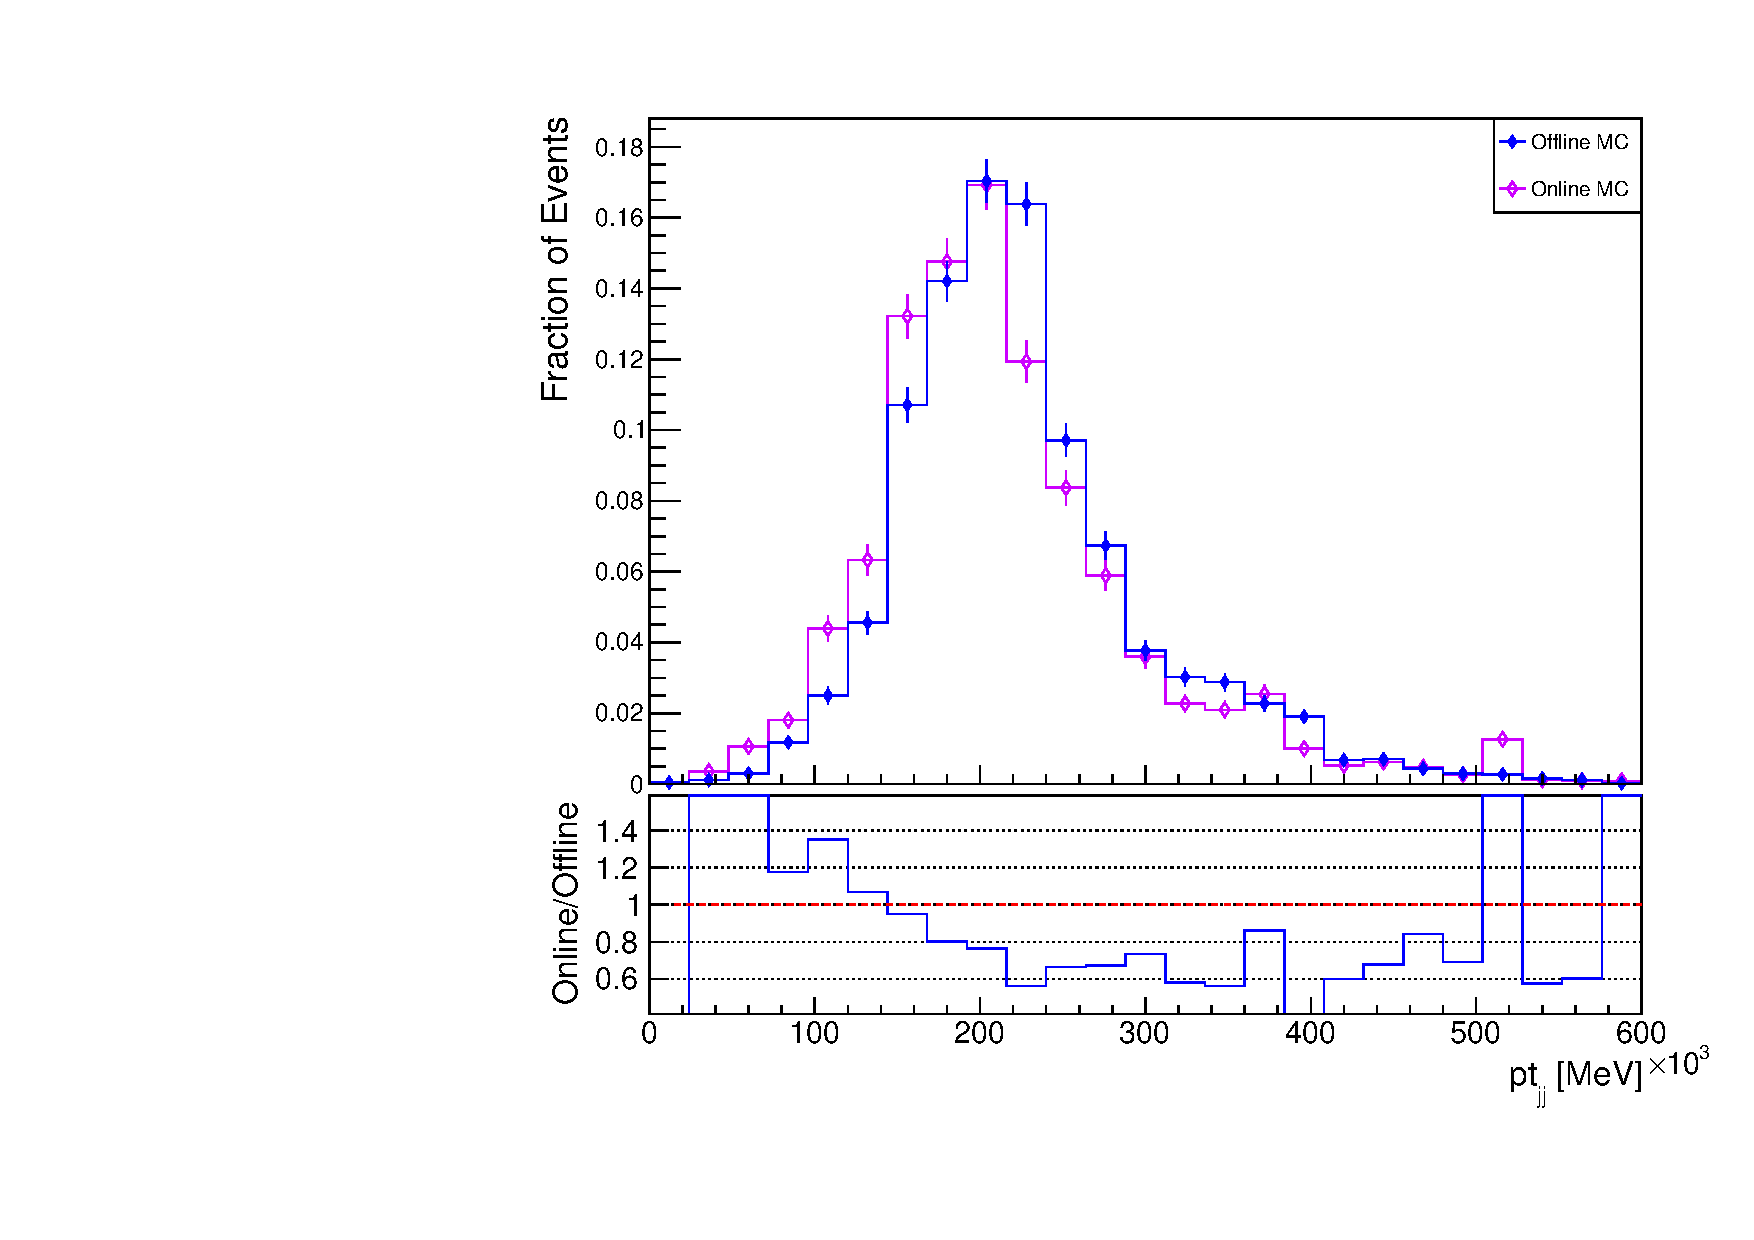
\includegraphics[width=1\linewidth]{ptjj_mc_}
            \end{minipage}
            \caption[Comparison of the \ptjj distribution of the \VBFHBB\ events for HLT and offline objects]{\ptjj distribution for the online and offline \VBFHBB\ events, with background events from data shown in the left panel and Monte-Carlo signal events in the right.}
        	\label{f:ptjj}
        \end{figure}

        \begin{figure}[h]
            \centering
            \begin{minipage}[h]{0.48\linewidth}
                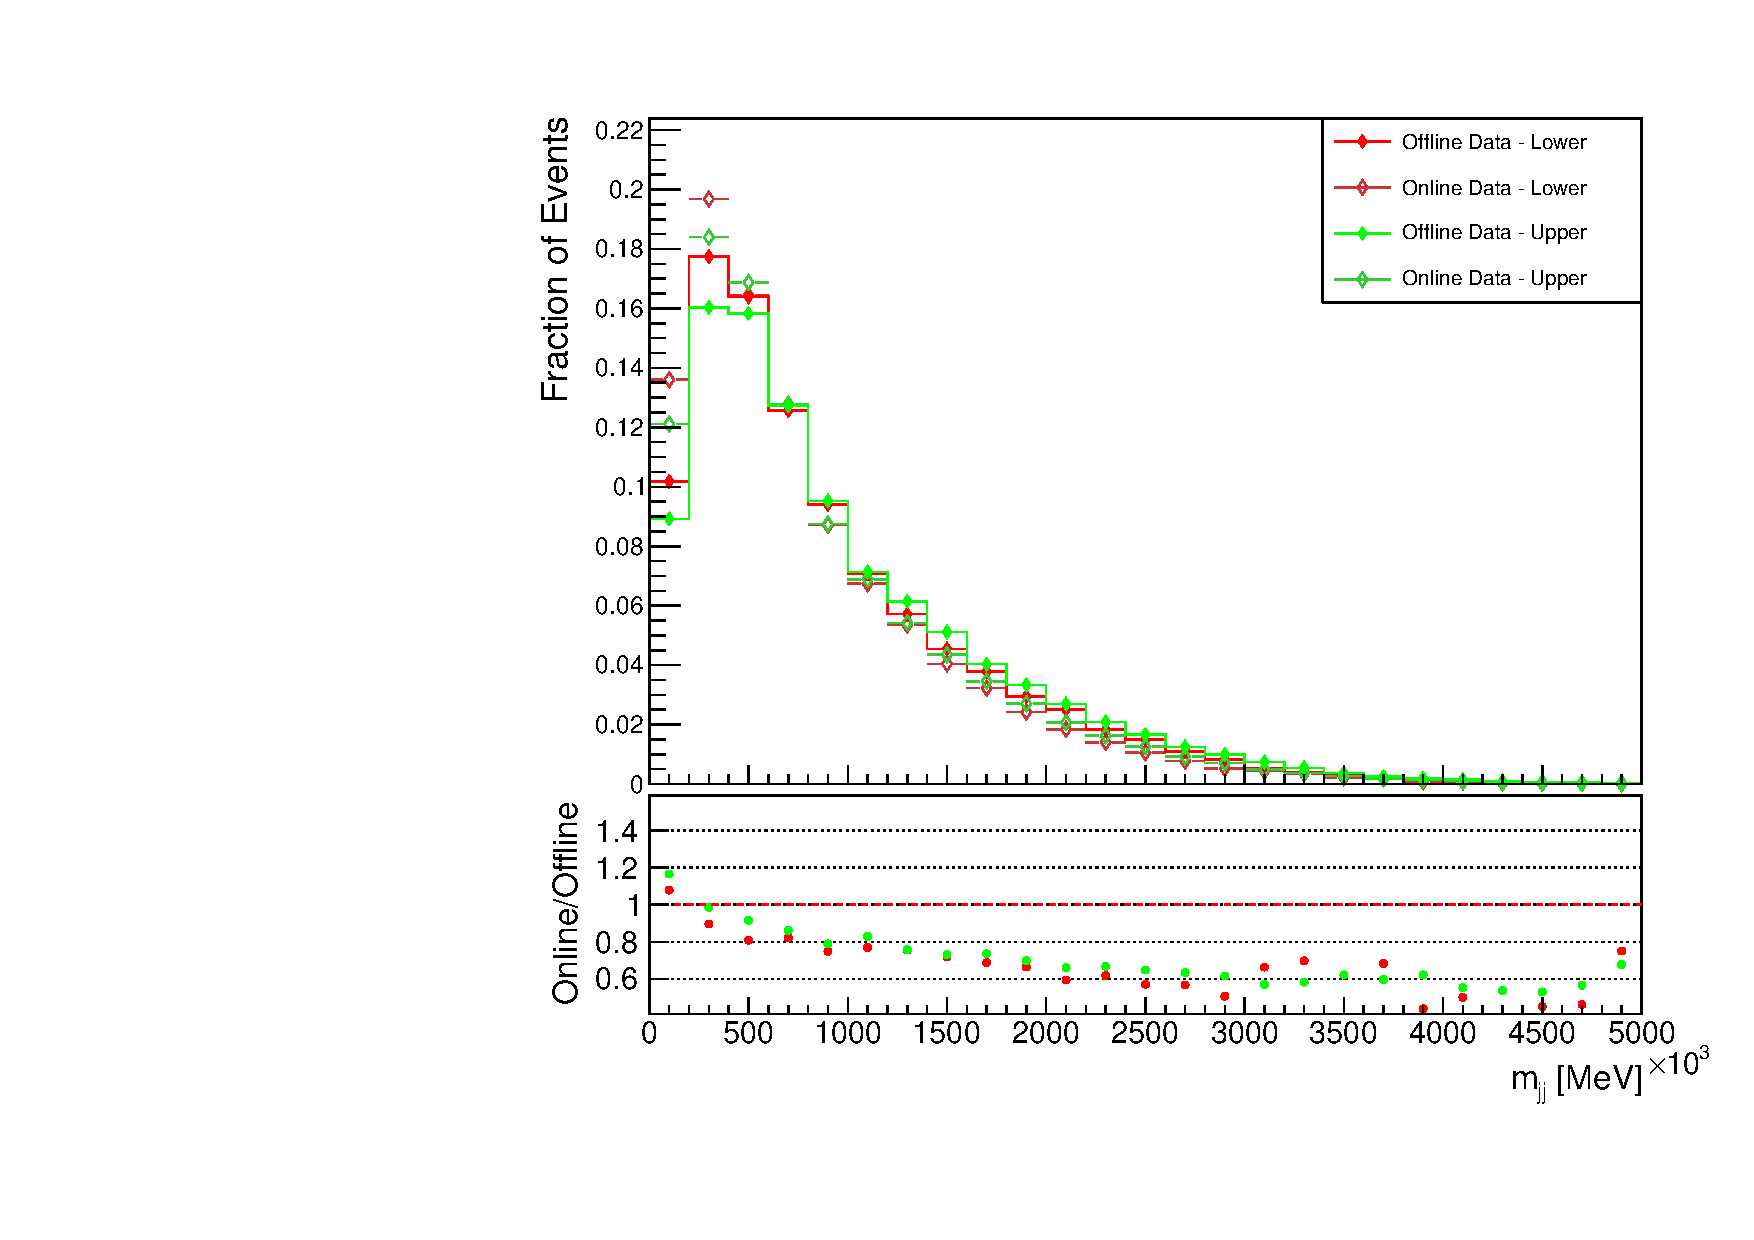
\includegraphics[width=1\linewidth]{mjj_data_}
            \end{minipage}
            \quad
            \begin{minipage}[h]{0.48\linewidth}
                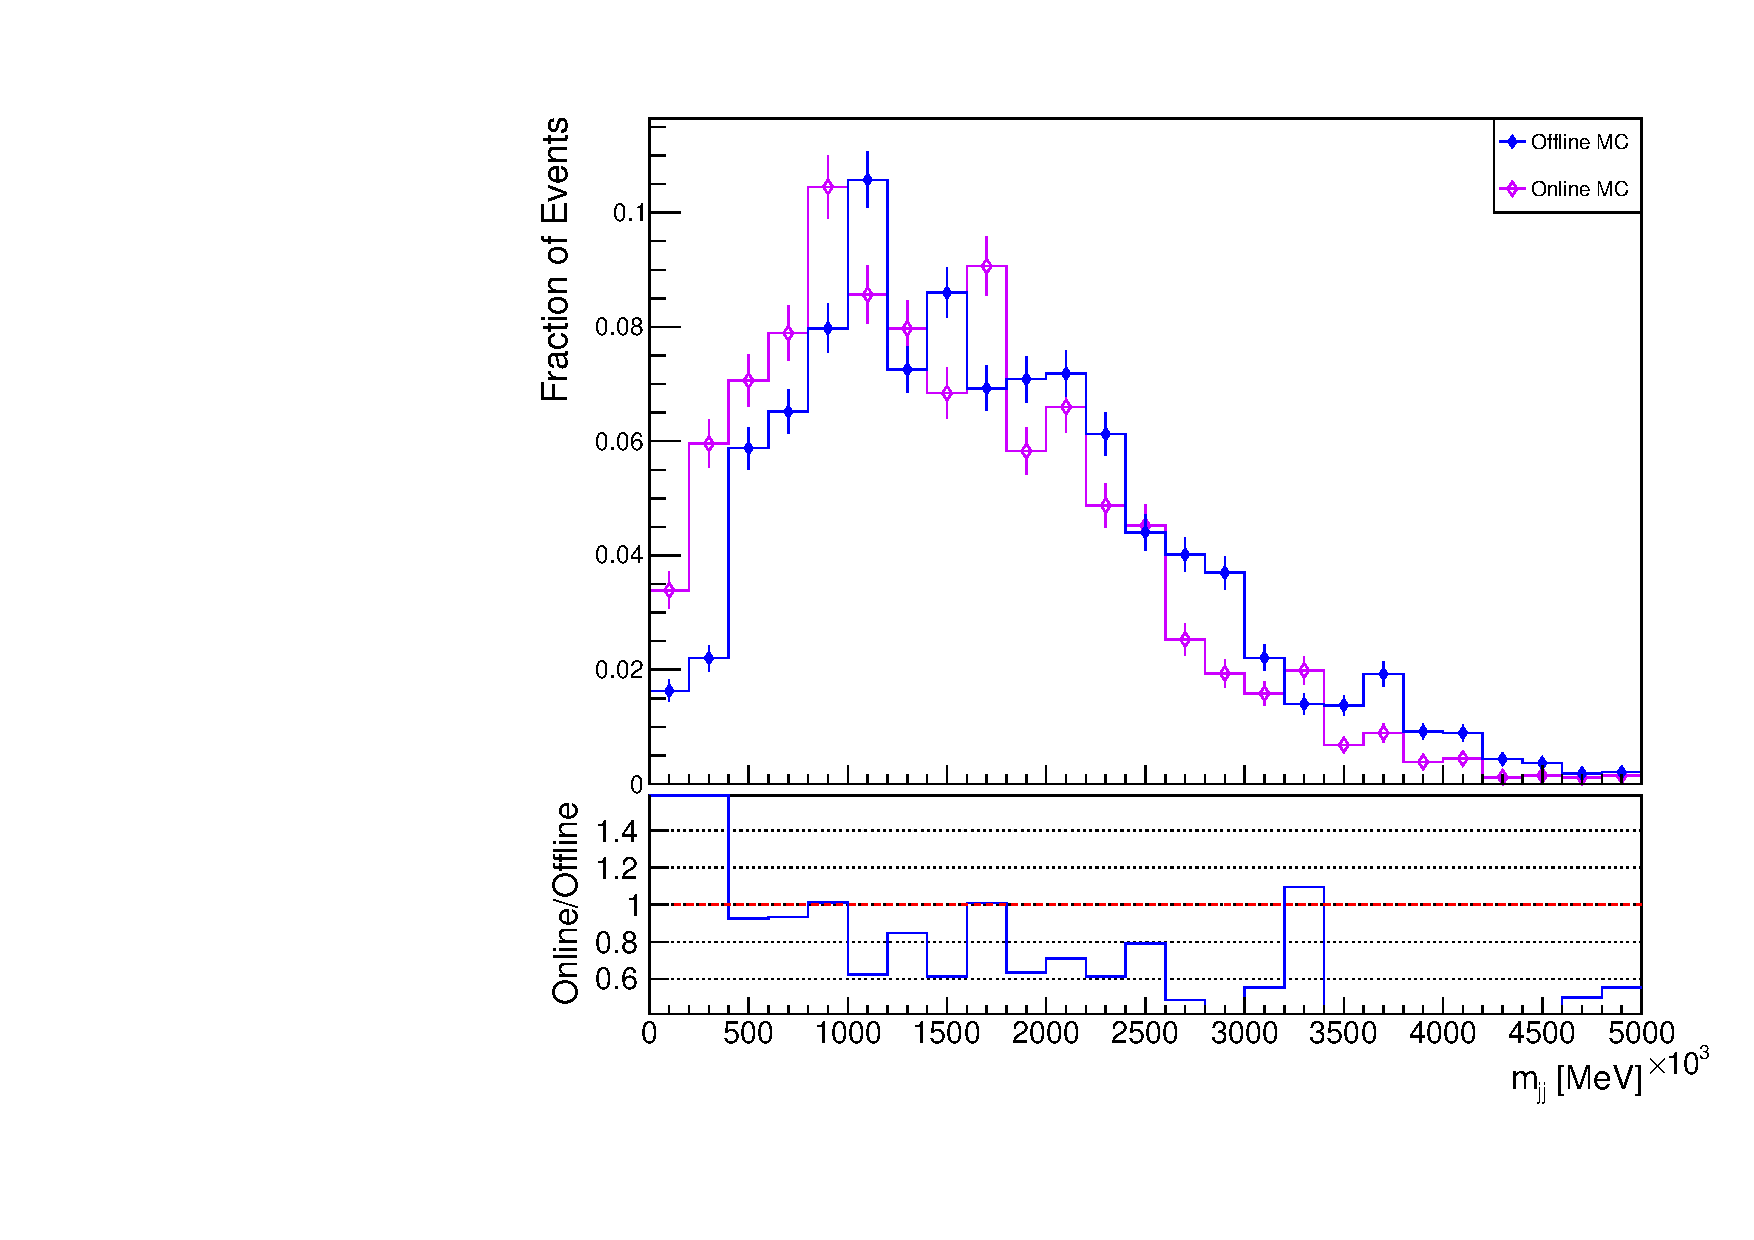
\includegraphics[width=1\linewidth]{mjj_mc_}
            \end{minipage}
            \caption[Comparison of the \mjj distribution of the \VBFHBB\ events for HLT and offline objects]{\mjj distribution for the online and offline \VBFHBB\ events, with background events from data shown in the left panel and Monte-Carlo signal events in the right.}
            \label{f:mjj}
        \end{figure}

        The \ptjj distributions shown in Figure \ref{f:ptjj} are similar to the plots of the leading non-\bjet\ shown in Figure \ref{f:ptj1}. The peak of the online distribution in the upper and lower background regions along with the signal region is shifted down in \ptjj in relation to the offline region. The overall shape of the distribution is consistent between the Monte-Carlo simulations and the data background regions, and the ratio plot shows similar characteristics to that in Figure \ref{f:ptj1}, flattening off at an online/offline ratio value of $\sim0.7$. These features are replicated in the \mjj plot in Figure \ref{f:mjj}: similar distributions shapes for upper background, lower background and signal, increased numbers of online events compared to offline events at low \mjj (which corresponds to low non-\bjet\ $p_\text{T}$), the online/offline ratio flattening off to a value of $\sim0.7$. These features, as described in Section \ref{k:jets} could be explained by the differences observed at low \pt regions for non-\bjets\ in Section \ref{OP:leadingnonb}. Overall the performance of online is comparable to offline, so these variables may be used to train a BDT and perform any further analysis using TLA methodologies.

        \begin{figure}[h]
            \centering
            \begin{minipage}[h]{0.48\linewidth}
                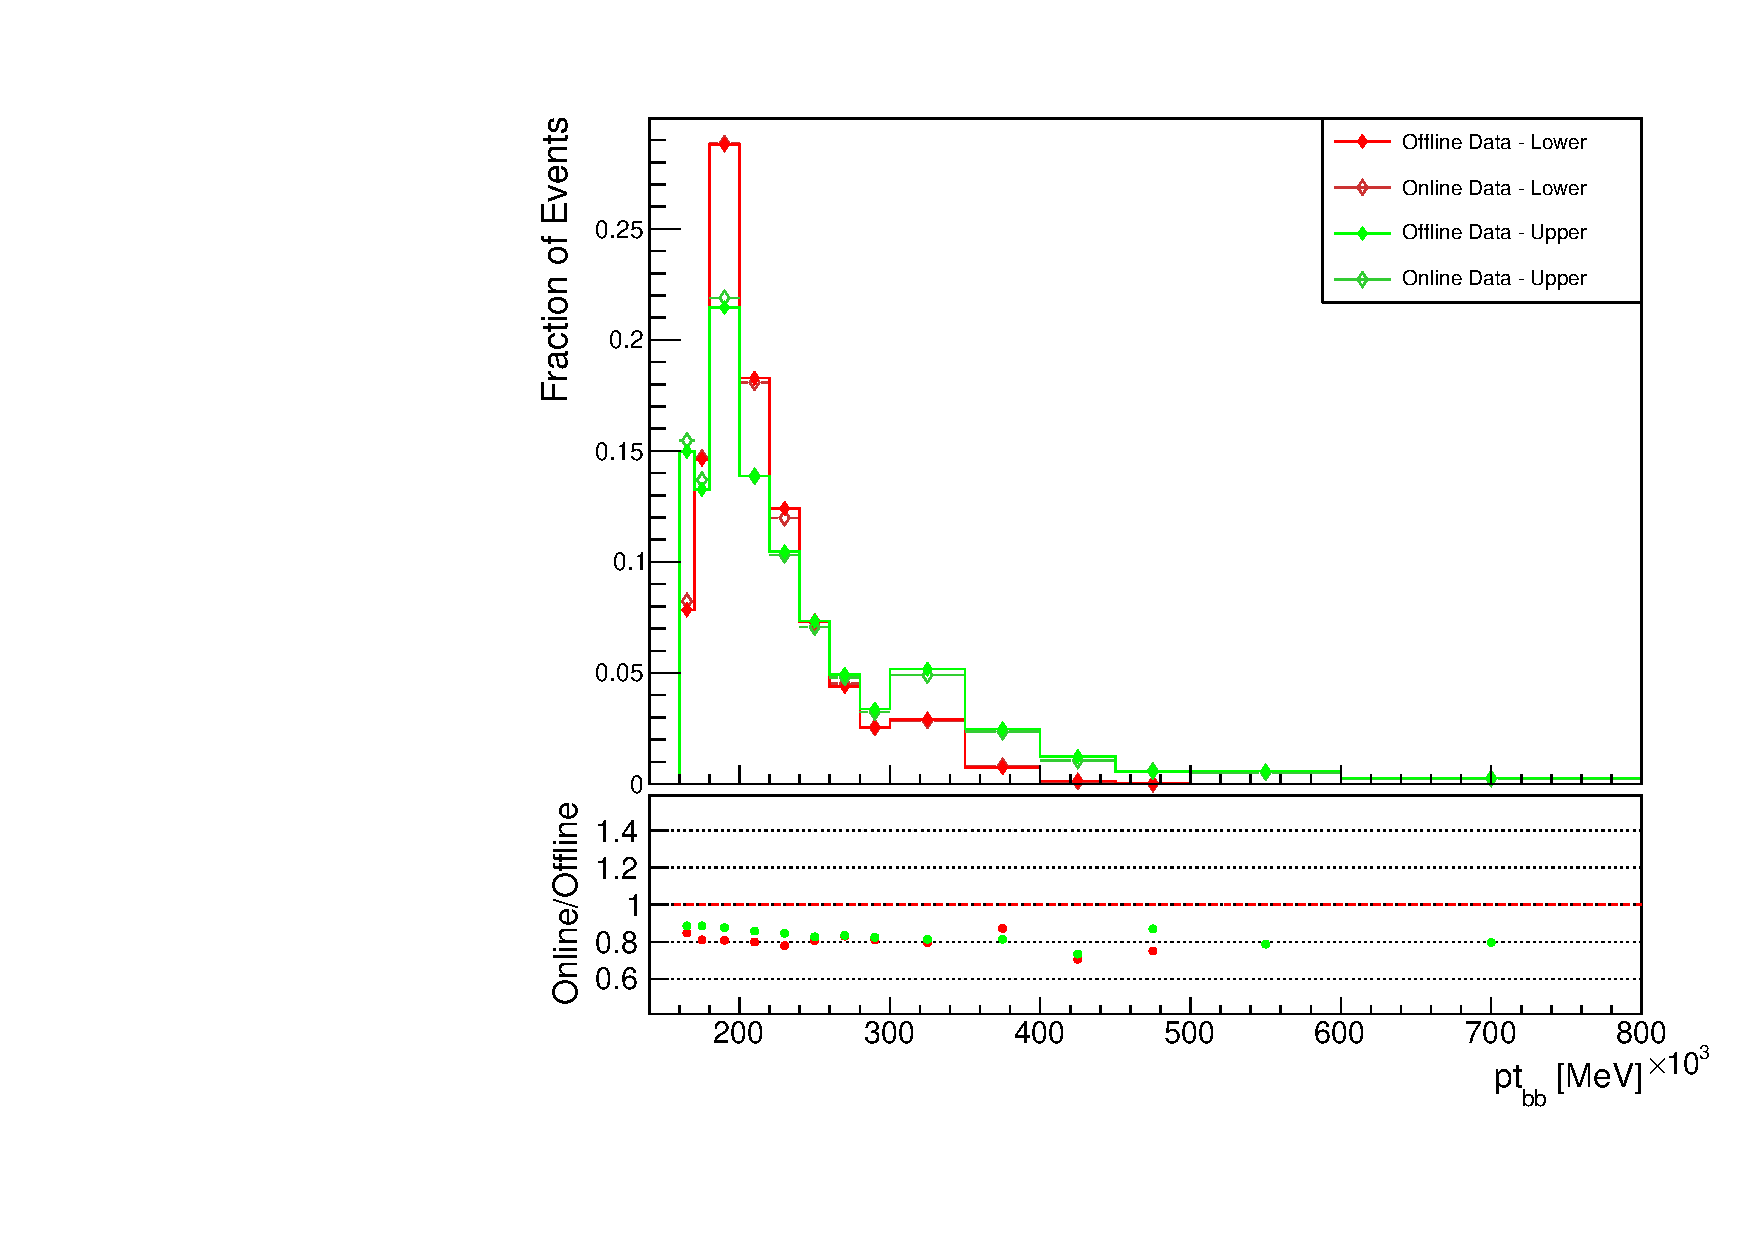
\includegraphics[width=1\linewidth]{ptbb_data_}
            \end{minipage}
            \quad
            \begin{minipage}[h]{0.48\linewidth}
                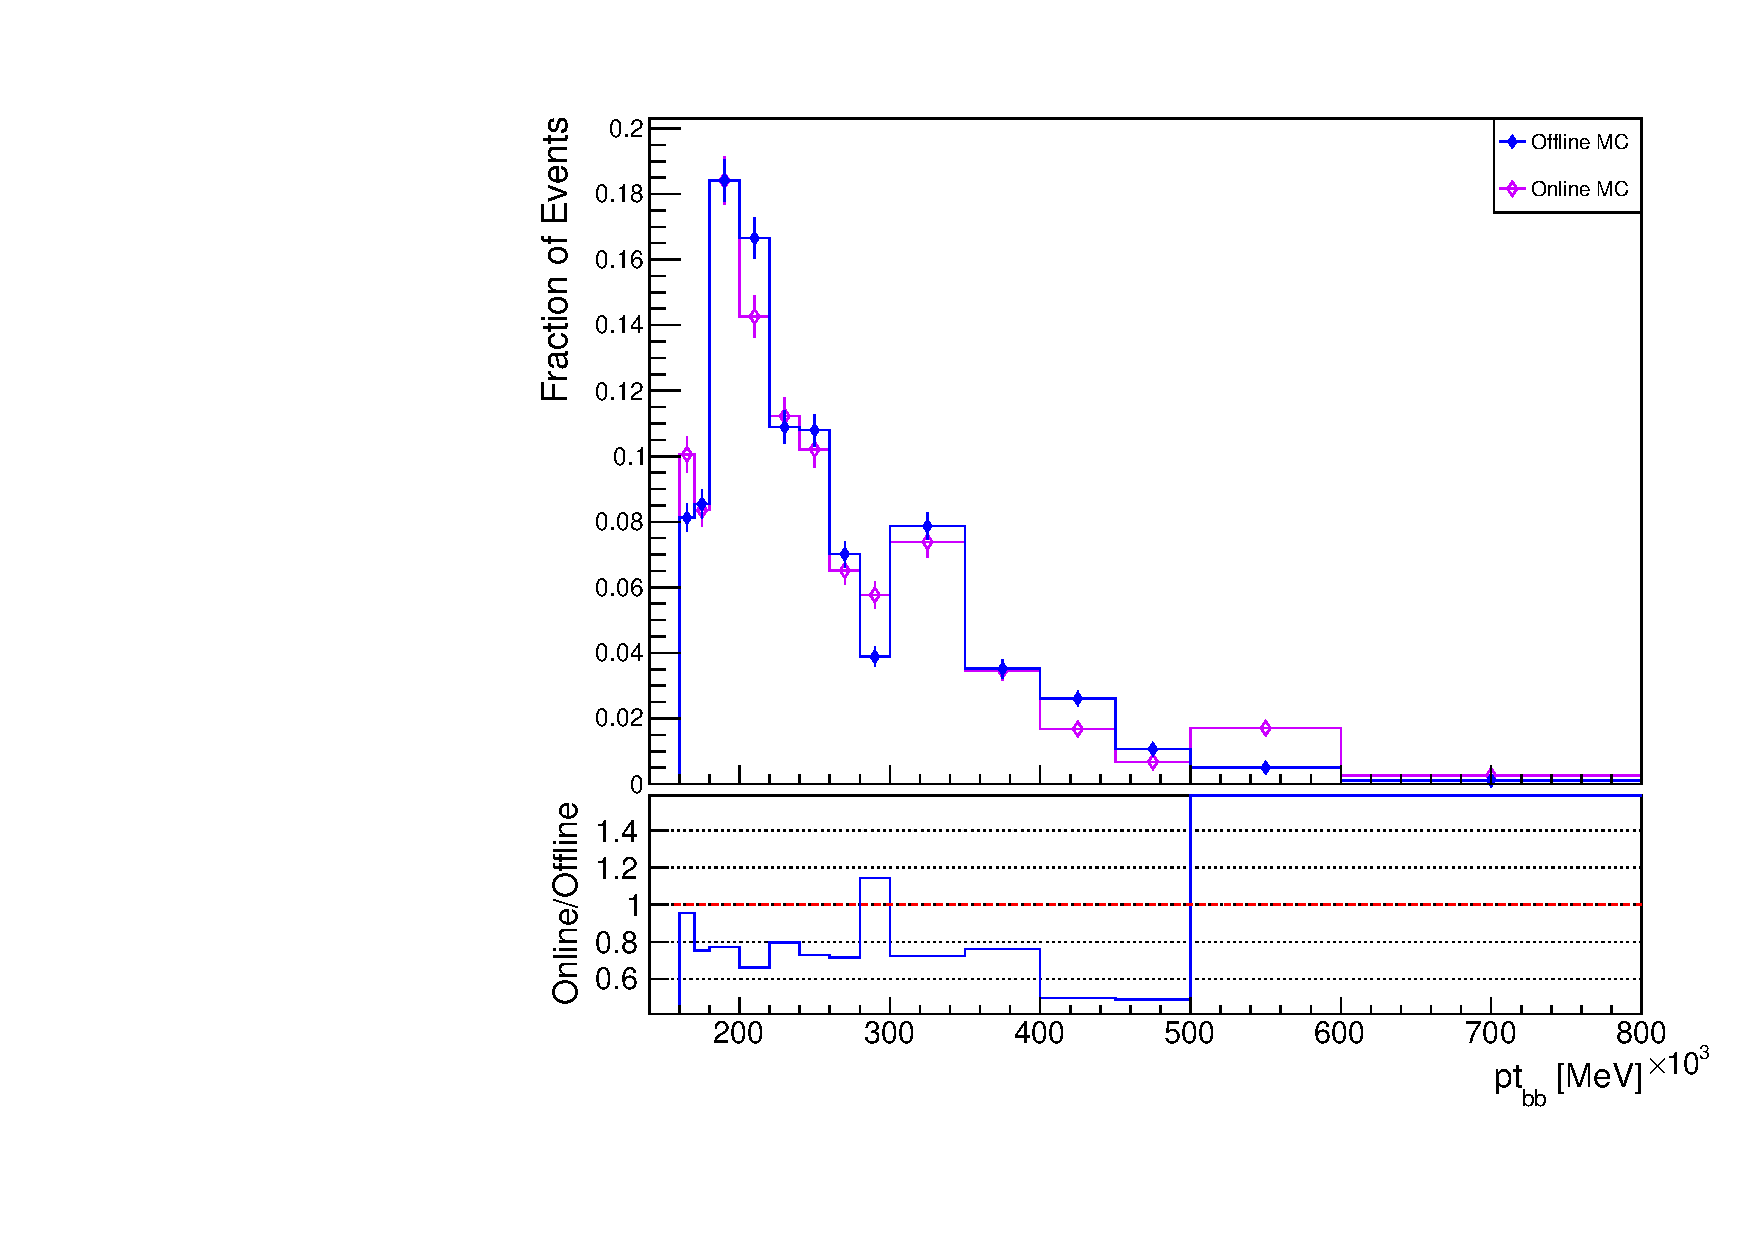
\includegraphics[width=1\linewidth]{ptbb_mc_}
            \end{minipage}
            \caption[Comparison of the \ptbb distribution of the \VBFHBB\ events for HLT and offline objects]{\ptbb distribution for the online and offline \VBFHBB\ events, with background events from data shown in the left panel and Monte-Carlo signal events in the right.}
            \label{f:ptbb}
        \end{figure}

        The plots of \ptbb in Figure \ref{f:ptbb} show excellent agreement between the online and offline objects. The ratio in the left panel of the Figure shows a flat line around $\sim0.8$, in strong agreement with the reduction in event count shown in Figure \ref{f:cutflowD}. This agreement with the expected decrease is also shown in the signal events, which agree with Figure \ref{f:cutflowMC}. For $p_{\text{T}bb}$, the same behaviour is seen for online and offline jets, indicating there is no additional problems for applying a TLA beyond the rate reduction.

        \begin{figure}[h]
            \centering
            \begin{minipage}[h]{0.48\linewidth}
                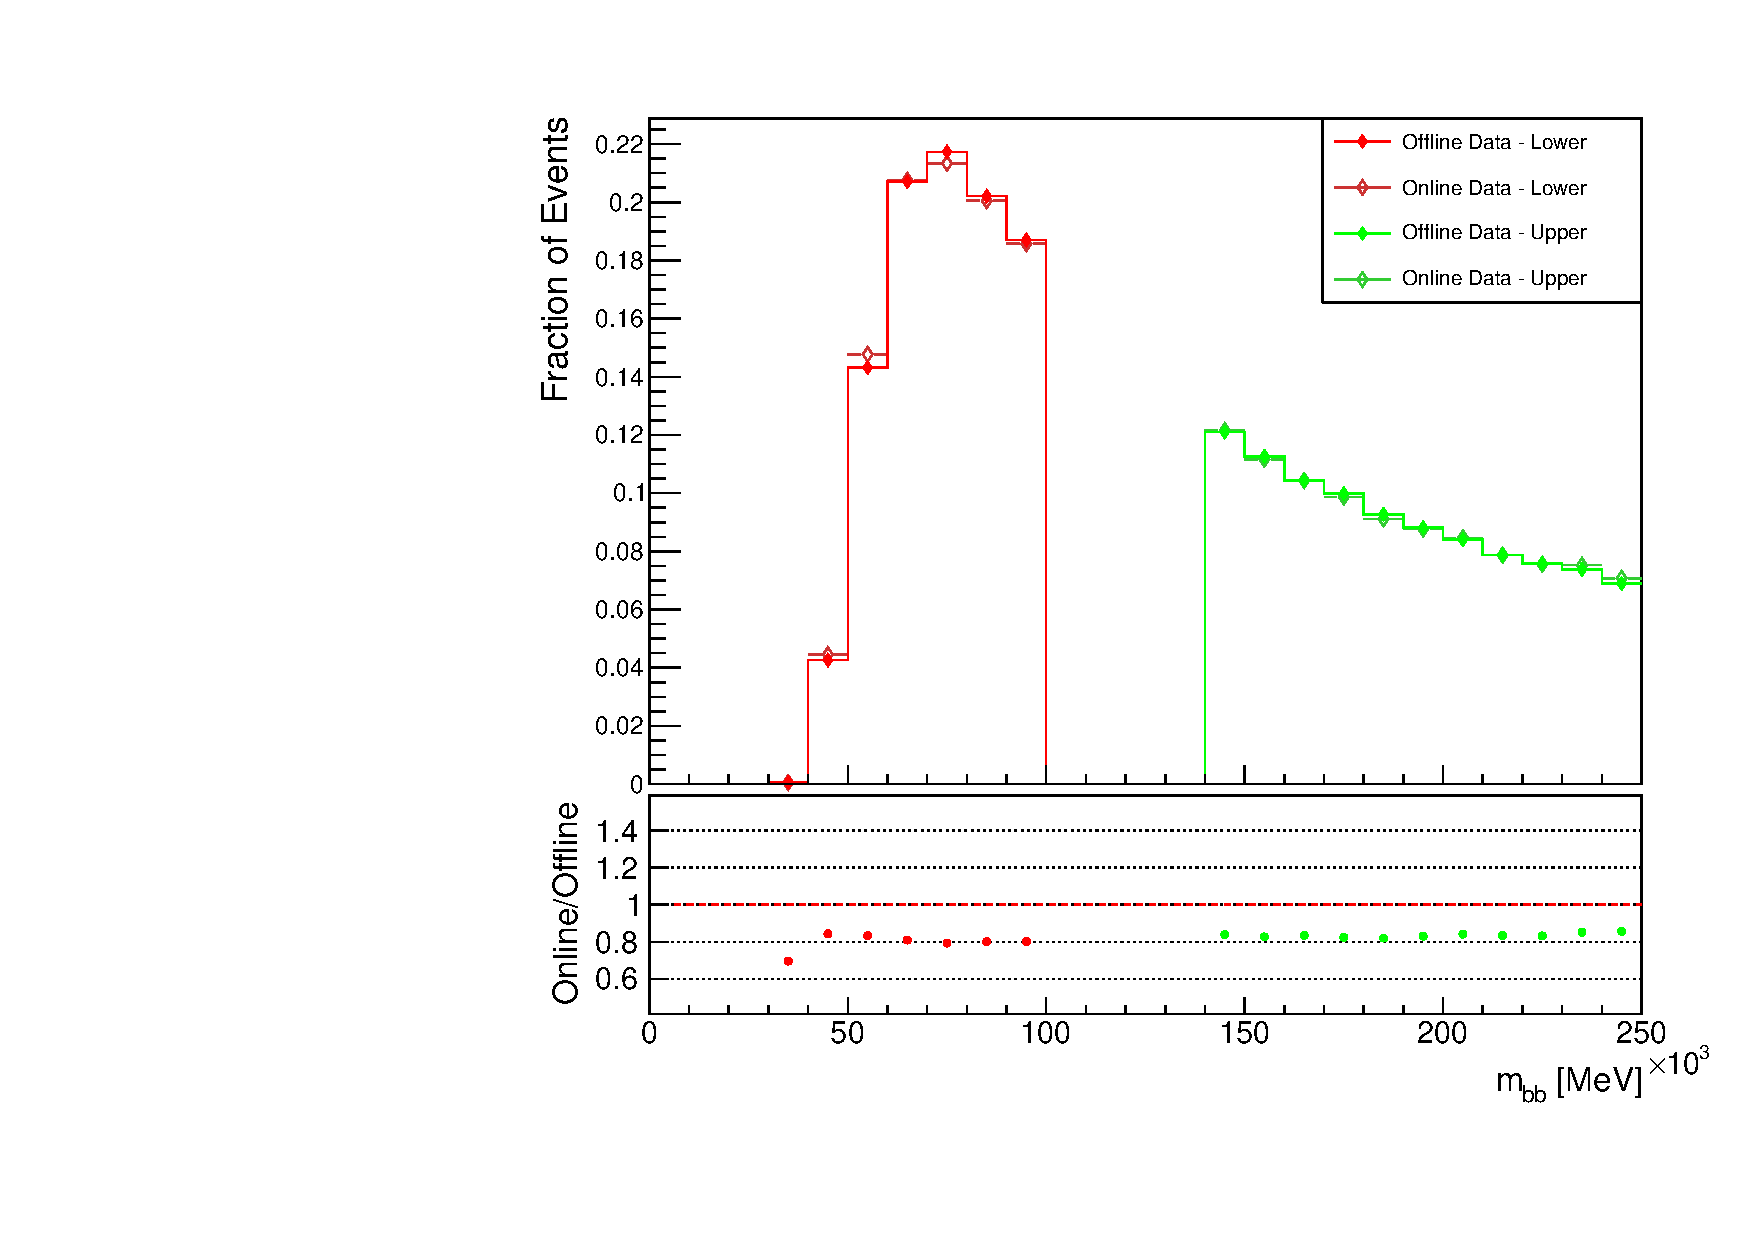
\includegraphics[width=1\linewidth]{mbb_data_}
            \end{minipage}
            \quad
            \begin{minipage}[h]{0.48\linewidth}
                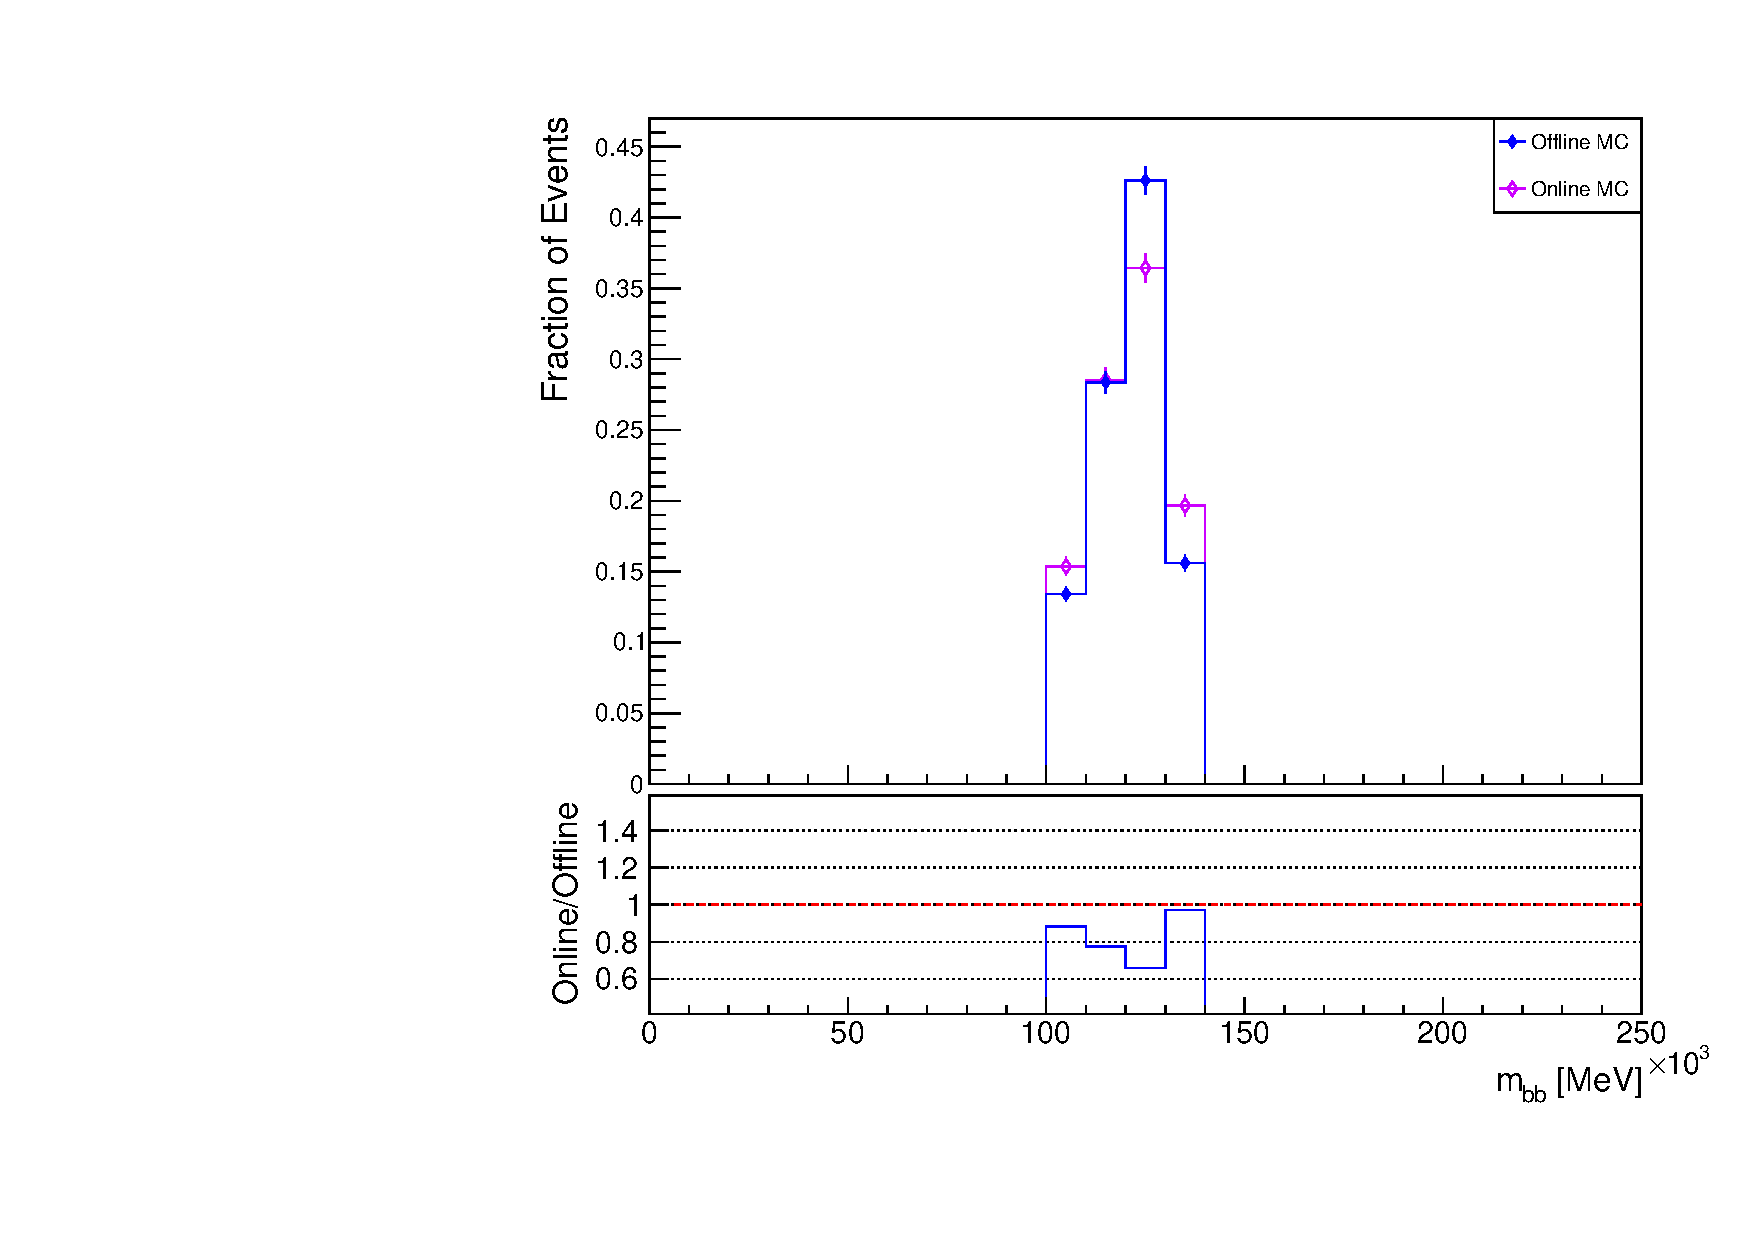
\includegraphics[width=1\linewidth]{mbb_mc_}
            \end{minipage}
            \caption[Comparison of the \mbb distribution of the \VBFHBB\ events for HLT and offline objects]{\mbb distribution for the online and offline \VBFHBB\ events, with background events from data shown in the left panel and Monte-Carlo signal events in the right.}
            \label{f:mbb}
        \end{figure}

        The \mbb plot in Figure \ref{f:mbb} for the background data events shows the online and offline analysis to be in good agreement. The online/offline ratio is a flat line at $\sim0.8$ as expected from the ratio plot in Figure \ref{f:cutflowD}. The behaviour of the upper and lower background region suggests a consistently decreasing function for \mbb beyond the peak at \pt$\sim80$GeV, and look to link up across the signal region. The signal region is less clear than the background data, but suggests a ratio value of $\sim0.8$ and shows comparable behaviour for the online and offline jets. As for the other kinematic quantities in this Section, the variables derived from the $b\bar{b}$ pair look to behave consistently for online and offline and so could be used in a TLA.
\section{BDT Input Variables}

    As discussed in Section \ref{es:as}, the full BDT analysis of the \VBFHBB\ search described in Appendix \ref{a:bdt} was not performed for this dissertation. Given this is a critical component of the full Higgs search \cite{VBFHbb8tev} in \VBFHBB, the performance of select BDT variables is explored for the signal and background regions described in Table \ref{t:signalback}. The variables \mjj and \ptjj covered in the previous section are both BDT training variables.

    This section covers $\eta^*$, given by

    \begin{equation}
    \eta^* = \frac{1}{2}(|\eta_{j1}| + |\eta_{j2}| - |\eta_{b1}| - |\eta_{b2}|)
    \end{equation}

    which is plotted in Figure \ref{f:etastar} for the online and offline events, and the \pt\textit{balance}, given by

    \begin{equation}
        p_{\text{T} balance} = \frac{\vec{p_{\text{T}j1}} + \vec{p_{\text{T}j2}} + \vec{p_{\text{T}b1}} + \vec{p_{\text{T}b2}}}{p_{\text{T}j1} + p_{\text{T}j2} + p_{\text{T}b1} + p_{\text{T}b2}}
    \end{equation}

    which is shown in Figure \ref{f:ptbalance}

    \begin{figure}[h]
        \centering
        \begin{minipage}[h]{0.48\linewidth}
            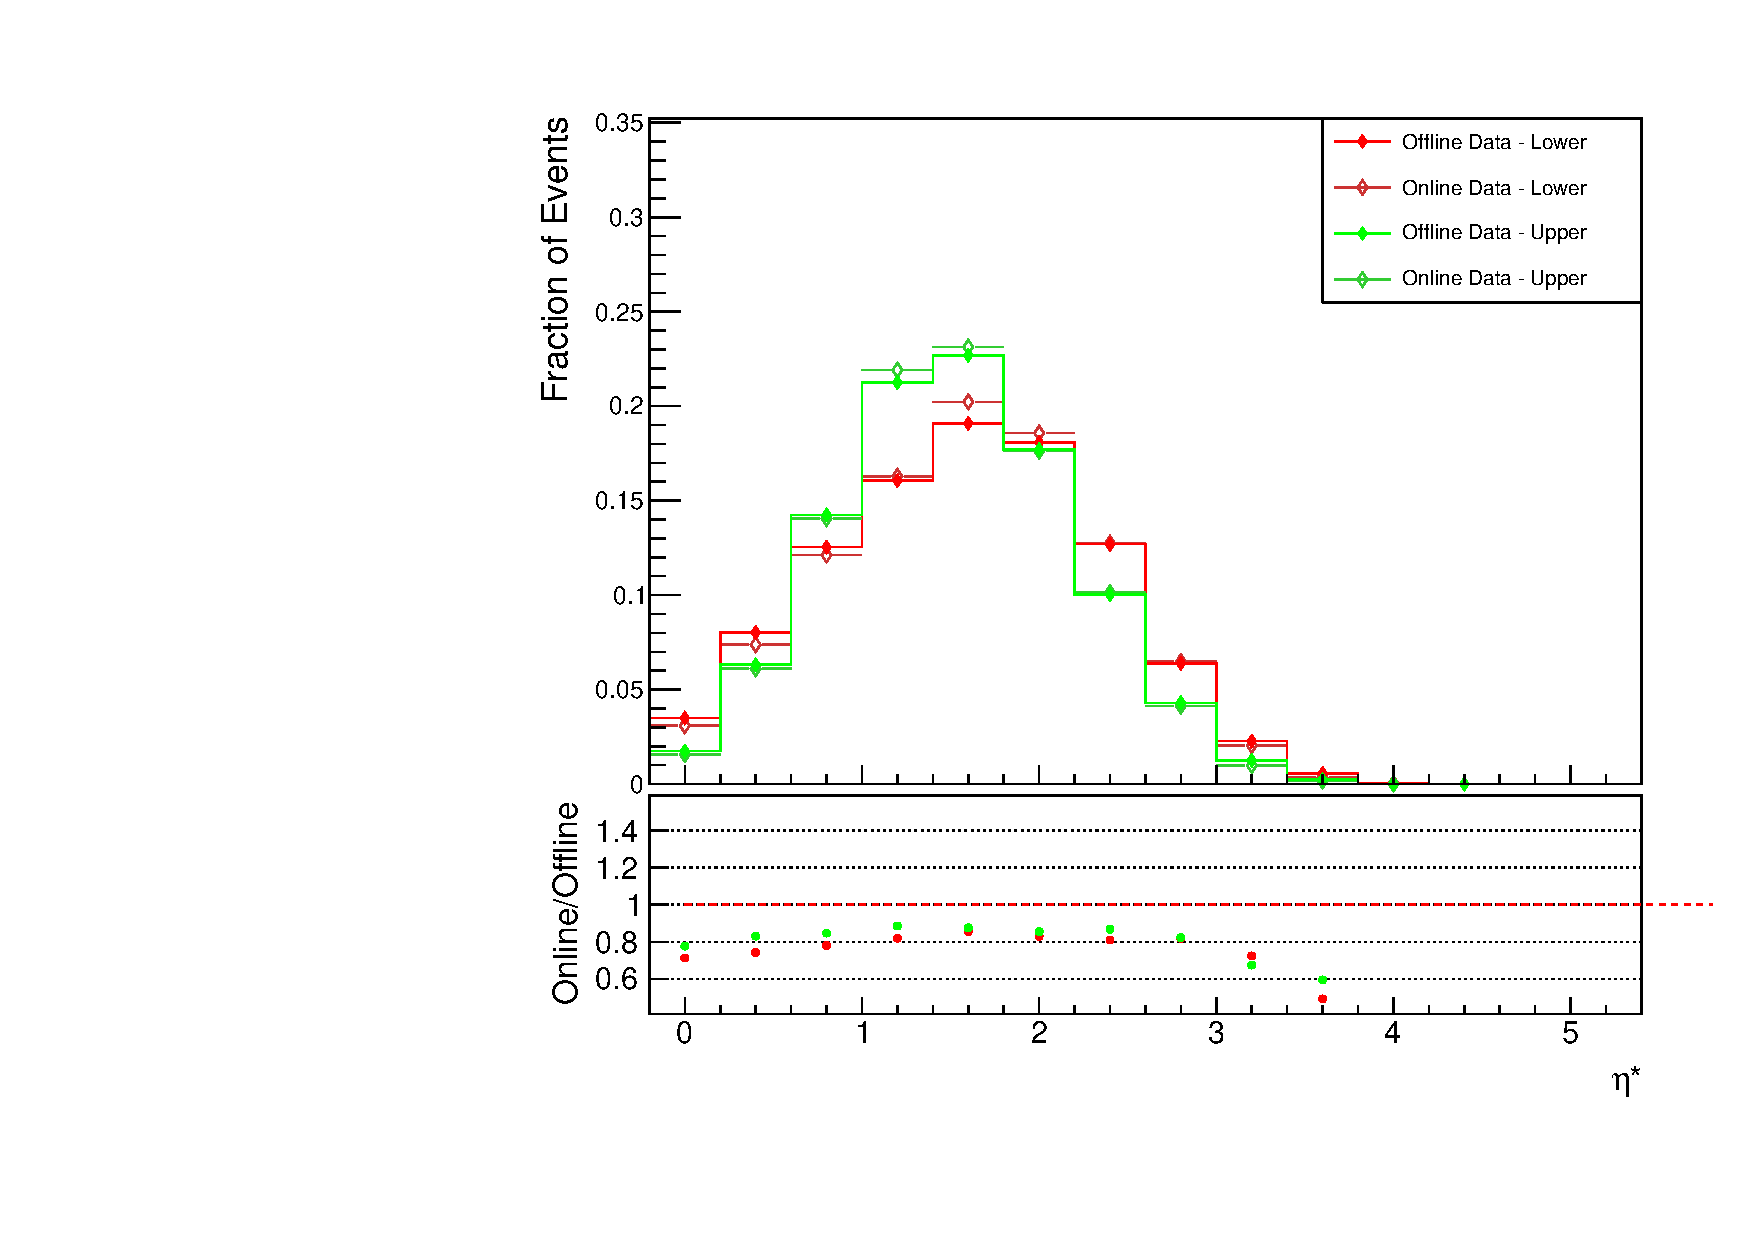
\includegraphics[width=1\linewidth]{etastar_data_}
        \end{minipage}
        \quad
        \begin{minipage}[h]{0.48\linewidth}
            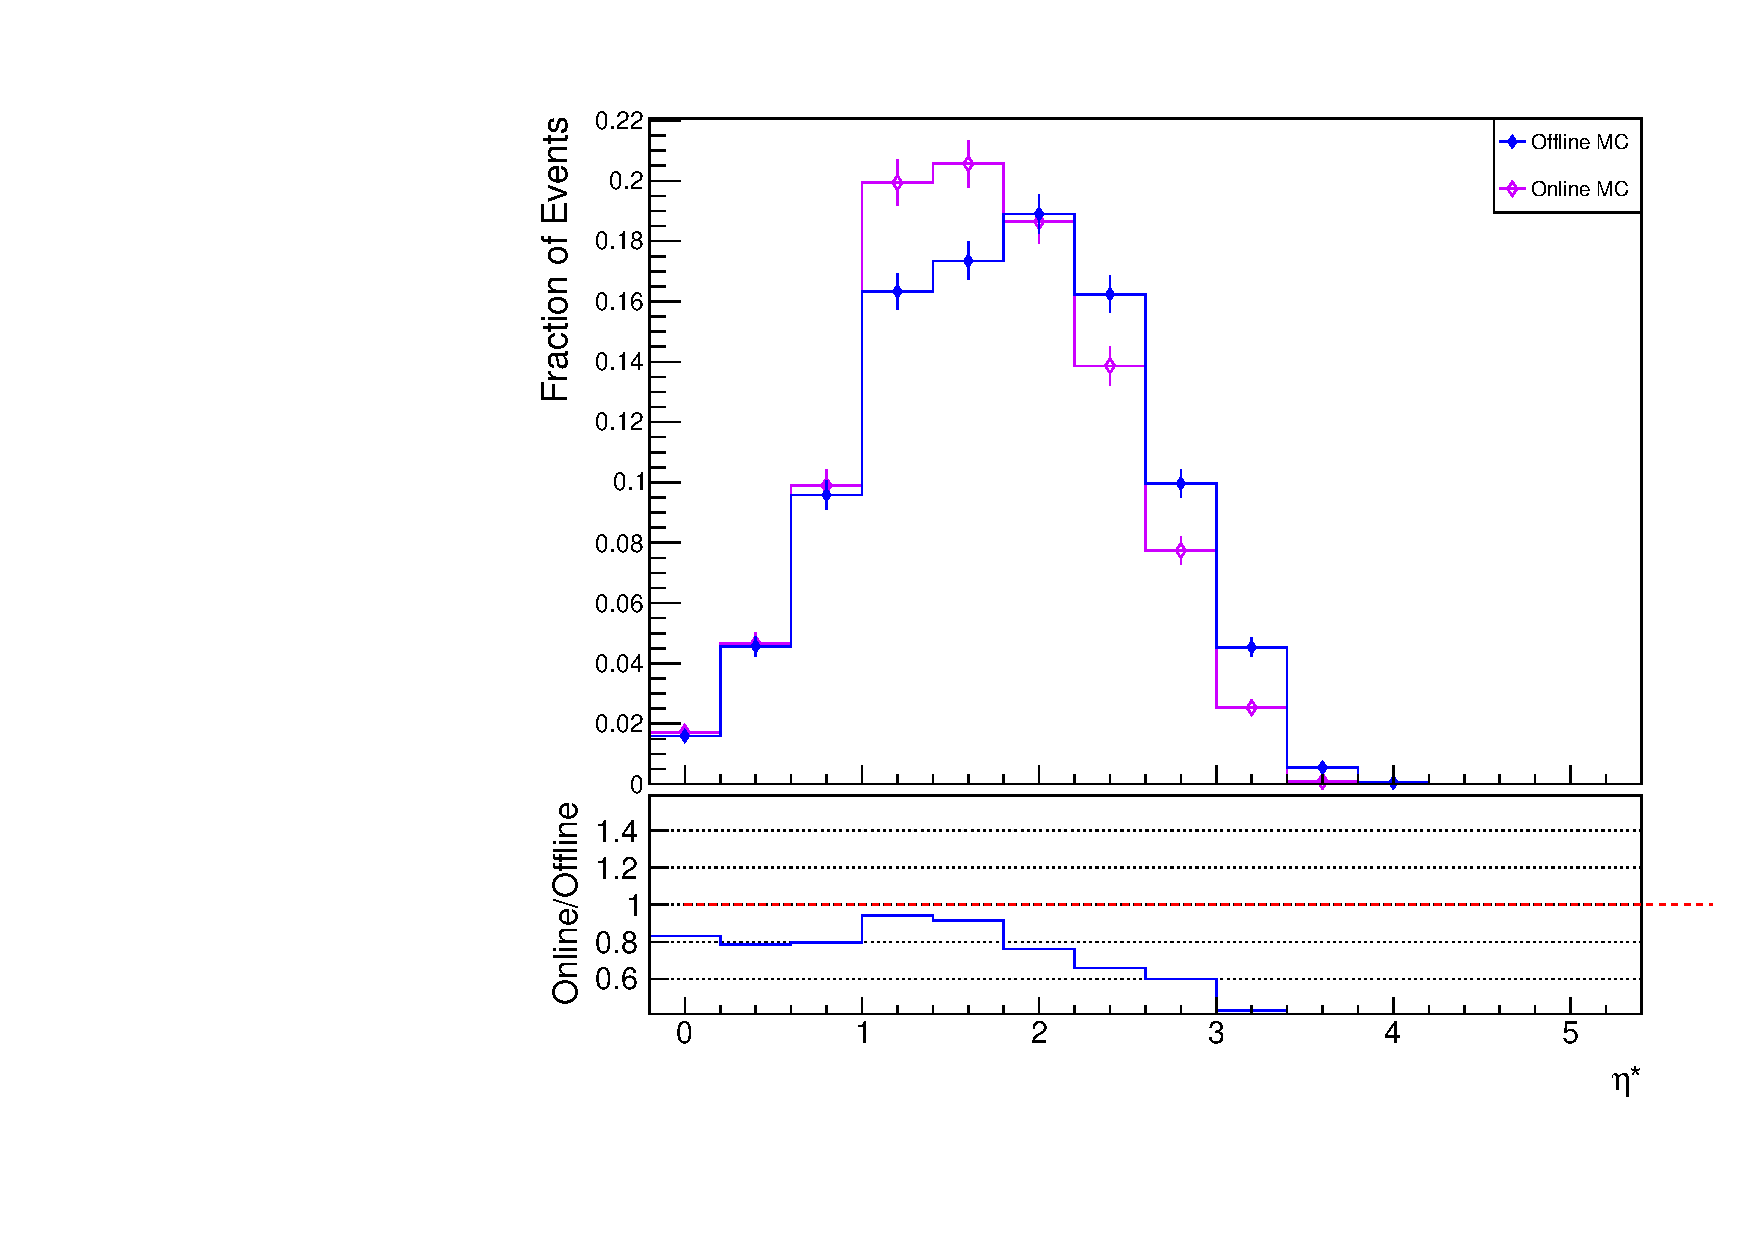
\includegraphics[width=1\linewidth]{etastar_mc_}
        \end{minipage}
        \caption[Comparison of the $\eta^*$ distribution of the \VBFHBB\ events for HLT and offline objects]{$\eta^*$ distribution for the online and offline \VBFHBB\ events, with background events from data shown in the left panel and Monte-Carlo signal events in the right.}
        \label{f:etastar}
    \end{figure}

    \begin{figure}[h]
        \centering
        \begin{minipage}[h]{0.48\linewidth}
            \includegraphics[width=1\linewidth]{ptbalance_data_}
        \end{minipage}
        \quad
        \begin{minipage}[h]{0.48\linewidth}
            \includegraphics[width=1\linewidth]{ptbalance_mc_}
        \end{minipage}
        \caption[Comparison of the $p_{\text{T} balance}$ distribution of the \VBFHBB\ events for HLT and offline objects]{$p_{\text{T} balance}$ distribution for the online and offline \VBFHBB\ events, with background events from data shown in the left panel and Monte-Carlo signal events in the right.}
        \label{f:ptbalance}
    \end{figure}

    These variables behave in a consistent fashion as to the other \VBFHBB\ kinematic quantities covered in this section. For the lower background, upper background and signal sectors the shapes of the online and offline curves are comparable. The relative ratio of the online to the offline events is $\sim0.8$, as covered in Section \ref{k:cutflow} and shown clearly by the ratio plots in the left panels of Figures \ref{f:etastar} and \ref{f:ptbalance}. The plots for the Monte-Carlo signal are less clear, but show a rough $20\%$ decrease in online events compared to offline, and in general the upper background region performs better than the lower region.

    Given the behaviour of the online and offline BDT quantities derived from the \VBFHBB\ event is similar, the trigger-level objects should perform comparably to the offline objects, and as such can be used in the training of a \VBFHBB\ BDT.
    \section{Summary}

    This chapter presents analysis and comparison of the \VBFHBB\ events obtained using trigger-level objects and offline reconstructions in data and Monte-Carlo simulation. The cutflows of the analysis for Monte-Carlo online, Monte-Carlo offline, data online and data offline were studied, and found to show online analysis produced $\sim82\%$ of the statistics of offline analysis for Monte-Carlo simulations, and $\sim84\%$ for data. These results are the overall decrease, the step by step changes of the cutflow were not predicted by the results from Chapter \ref{c:OP}. Section \ref{k:cutflow} contains discussion of some possible causes, and they could also be the result of some coding bugs in the analysis.

    With this reduction of event yield for a given analysis sample, the increased trigger rates permitted when applying TLA will result in an increased final event count. For current rate increases in TLA analyses \cite{tla}, this would amount to an increase of $\sim66\%$ in the final number of events. This estimate of the possible increase does not consider any limitations on the rate that may result from increased computational demands on either processing or TLA object byte size.

    To confirm that the TLA analysis would be possible with the trigger-level objects, the component jets, kinematic properties of the \VBFHBB\ event and select BDT training variables were investigated. These cases showed consistent behaviour between the online and offline objects in both background data and signal Monte-Carlo simulation, while showing the online rate decrease calculated from the cutflows.

    These results suggest a full study of \VBFHBB\ analysis is a feasible proposal. Use of TLA could increase the output rate of the triggers to statistically significant levels and the objects produced will behave during analysis in a consistent fashion to the offline objects.
\endinput


\chapter{Conclusions}
\label{c:c}

This dissertation contains work done to test the feasibility of using Trigger-Object Level Analysis to improve the statistical significance of searches for the Higgs boson produced via Vector Boson Fusion and decaying to bottom quarks. This feasibility was tested by assessing the performance of trigger-level online analysis compared to the reconstructed offline analysis at two levels of abstraction for the \VBFHBB\ event, firstly at the resolution of comparing the performance for the individual jet objects that make up a \VBFHBB\ event separate from the \VBFHBB\ topology, and then by performing elements of the full \VBFHBB\ analysis with both online and offline objects to compare the performance.

The analysis was carried out using a vector boson fusion Monte-Carlo simulation sample and $4.63$~fb$^{-1}$ of data collected by the ATLAS detector during data-taking period D of the 2016 $\sqrt{s}=13$~TeV Run.

The individual online and offline jet objects were shown to be comparable to each other, and could be improved to show a closer agreement in behaviour using standard ATLAS analysis tools. The positions of the \bjets\ and non-\bjets\ that make up a \VBFHBB\ event were shown to agree within $1\%$ of each other in ($\eta$, $\phi$) space. The \pt distributions of the online and offline jets demonstrated small differences, with offline \pt being $\sim5\%$ larger than online \pt for both the \bjets\ and the non-\bjets. This \pt difference arises from a difference in the jet energy scale calibrations of the online and offline jet objects, and can be rectified in future analyses using standard jet calibration tools.

The \btag\ performance of the individual jet objects were compared, which showed differences in the \btag\ efficiency, \cjet\ rejection and light-jet rejection between the online and offline jets. These differences in efficiency were consistent with the expected change in performance  resulting from the different \btag\ algorithms applied to the online and offline jets. The 2016 MV2c10 \btag\ algorithm to the offline reconstructed jets, while the \btag\ information for the online jets was calculated using the 2015 MV2c20 algorithm that was operational in the detector at that time. This suggests \btag\ performance of the online objects can be brought closer to agreement if the \btag\ training variables are preserved on the trigger-level objects, rather than being discarded and leaving only the \btag\ decision in the DxAOD. However, the performance of the algorithms underpinning the MV2 algorithms (Section \ref{det:btagging}) will also be improved over time, so the training variables will still differ from the offline reconstructions. In addition, the tracking will differ online to offline, so it is unlikely online performance could be brought to equivalence with offline performance.

Comparison of the online and offline performance in a \VBFHBB\ event phase space was then carried out. These cuts resulted in a final online event count that was reduced relative to the offline event count, with a final online event fraction of $82\%$ for Monte-Carlo simulation and $84\%$ for data. With the increased trigger rate permitted by using TLA, this would on average increase the final event number by $66\%$ relative to a purely offline analysis.

Finally the \VBFHBB\ event specific objects, kinematic quantities and BDT training variables were compared for the online and offline events. For each separate variable, the performance of the online analysis was broadly consistent with respect to the offline analysis, taking into account the reduction in the number of online events highlighted during the cutflow analysis. These results suggest that TLA analysis in the \VBFHBB\ channel will provide increased statistical significance while providing comparable events to the full offline reconstructed analysis.

The work of this dissertation suggests certain additional studies outside the scope of this analysis should be carried out prior to approving TLA for the \VBFHBB\ channel. Primarily, the practicalities of applying TLA in the \VBFHBB\ channel require assessment. The solutions proposed in this dissertation to improve the agreement between the online and offline objects will increase the size of the trigger-objects output by the detector and may result in additional computational cost in the HLT. This may result in a smaller rate increase than assumed based on prior TLA studies and reduce or remove the improvement in rate suggested here. Another avenue for improving the agreement would be to run improved \btag, tracking and jet calibrations online to make it more comparable. Also, the increased trigger rate from a TLA may be sufficient even given the drop in efficiency with TLA.

In addition, the comparative behaviour of the online and offline objects could have further verification steps. This work did not implement trigger emulation in the Monte-Carlo simulations, and this resulted in discrepancies between the Monte-Carlo and data results for the jet object performance. The full \VBFHBB\ analysis performed at $\sqrt{s}=8$TeV carried out a BDT analysis after the cuts implemented in this dissertation to enhance the \VBFHBB\ phase space. Implementing or retraining a BDT was not possible within this dissertation, but would be an informative branch of further work to verify the feasibility. Finally, technical limitations prohibited making use of the full data set produced by the ATLAS detector, so analysis was carried out on a subset of the data. Greater statistical significance and a more certain statement of similarity could be made by performing the analysis for a larger dataset.

This study on the feasibilty of performing TLA on the \VBFHBB\ channel search for the Higgs boson suggests that the trigger-level objects used for a \VBFHBB\ analysis are comparable to the offline objects, and that the similarity can be improved with some readily available calibrations and adjustments to the trigger-level objects. Also, the final \VBFHBB\ event produced using trigger-level objects will show a worse efficiency compared to offline reconstruction, but with the trigger rate increase afforded by TLA produce more events than an offline analysis. These additional events will be comparable in behaviour to the offline reconstruction. There are some additional sections of work relating to implementing and completely verifying the conclusions of this dissertation, but overall trigger-object level analysis is suggested as a feasable analysis strategy in the search for the Higgs boson via the \VBFHBB\ channel.


%
% appendices...
%
\appendix

\chapter{Configuration}\label{a:config}

This appendix details the files and configuration settings used referenced throughout.

\section{Files}
    \begin{table}[h]
        \caption{Full filenames of samples and other files used during the analysis}
        \label{t:files}
        \medskip
        \centering
        \begin{tabularx}{\textwidth}{p{4.5cm} X}\toprule
            Title & Filename \\\midrule

            2016 $25$ns Good Runs List & \texttt{data16\_13TeV.periodAllYear\_DetStatus-v88\-pro20-21\_DQDefects\-00-02-04\_PHYS\_Standard\linebreak GRL\_All\_Good\_25ns.xml}\\
            2016 13TeV \texttt{HIGG5D3} sample & \texttt{data16\_13TeV.\{RUN\_ID\}.physics\_Main.merge.\linebreak DAOD\_HIGG5D3.f715\_m1620\_p2689\_tid\{TID\}} \\
            MC15C \texttt{HIGG5D3} derivation Monte-Carlo sample & \texttt{mc15\_13TeV.341566.PowhegPythia8EvtGen\linebreak\_CT10\_AZNLOCTEQ6L1\_VBFH125\_bb.merge.\linebreak DAOD\_HIGG5D3.e3988\_s2726\_r7772\_r7676\_p2719} \\\bottomrule
        \end{tabularx}\\[5pt]
    \end{table}
\newpage
\section{Configurations}
    \begin{table}[h]
        \caption{Full names of configurations used during the analysis}
        \label{t:config}
        \medskip
        \centering
        \begin{tabularx}{\textwidth}{p{4.5cm} X}\toprule
            Title & Name \\\midrule
            Real Data 20.7 Jet Calibration Recommendations & \texttt{\detokenize{JES_data2016_data2015_Recommendation_Dec2016.config}} \\
            Monte-Carlo 20.7 Jet Calibration Recommendations & \texttt{\detokenize{JES_MC15cRecommendation_May2016.config}} \\
            January 2017 MV2c10 \btag\, Recommendations & \texttt{\detokenize{2016-20_7-13TeV-MC15-CDI-2017-01-31_v1.root}}\\
            March 2016 MV2c20 \btag\, Recommendations  & \texttt{ \detokenize{2016-Winter-13TeV-MC15-CDI-March10_v1.root}}\\\bottomrule
        \end{tabularx}\\[5pt]
    \end{table}
\endinput


\chapter{Boosted Decision Trees}\label{a:bdt}

This appendix gives a brief description of the definition and use of Boosted Decision Trees (BDT), and provides specific details as to the training of a BDT for a \VBFHBB\, analysis.

\section{Machine Learning}

A BDT is a machine learning technique that is applied in analyses to separate signal events from background events. The tree is trained on a particular training sample to build the decision logic and then applied to real data as required.

A decision tree as a structure operates by taking variables from the event and creating nodes with child nodes split on ranges of the variables. By assessing the relative signal/background proportions of the child nodes of this split node, the tree can create a split where one side is mostly signal and one mostly background. This process can be applied repeatedly to generate a multiple level tree of decision nodes, iteratively splitting sections of the event dataset. At a final terminating leaf node of the tree, the proportions of the signal and background events in the node will label it as a signal node or a background node.

This structure once trained, can be used to label a measured event by moving down the tree and evaluating each decision before a leaf node is reached in order to categorise the event. The boosting of a decision tree refers to the process of applying weights to the events. The tree will be iteratively produced, reweighting any misclassified events at each iterative stage to produce a more refined final tree \cite{bdt}. Such structures are used throughout modern physics analyses at ATLAS \cite{mlbtag}.

\section{\VBFHBB\, BDT Training}

A detailed description of the BDT training that should be carried out for a \VBFHBB\, search is given in Ref. \cite{VBFHbb8tev}. The event variables used for training the BDT on the \VBFHBB\, events are summarised here.

    \begin{table}[h]
        \caption{BDT Variables used in training for the \VBFHBB\, analysis.}
        \label{t:BDTvars}
        \medskip
        \centering
        \begin{tabularx}{\textwidth}{p{4.5cm} X}\toprule
            Variable & Description \\\midrule
            $M_{jj}$ & Invariant mass of the VBF jet pair. \\
            \ptjj & Transverse momentum of the VBF jet pair \\
            $\cos\theta$ & Cosine of the polar angle of the cross product of the VBF jet momenta in the Higgs rest frame. \\
            $Max(\eta)$ & $max(|\eta_{j1}|, |\eta_{j2}|)$ Maximum of the two absolute pseudorapidity values for the VBf jets. \\
            $\eta *$ & $\frac{1}{2}(|\eta_{j1}| + |\eta_{j2}| - |\eta_{b1}| - |\eta_{b2}|)$ Average pseudorapidity difference between the VBF and signal jets. \\\
            $min\Delta R_{j1}$ & Minimum ($\eta, \phi$) separation between the leading VBF jet and the closest other jet.\\
            $min\Delta R_{j2}$ & Minimum ($\eta, \phi$) separation between the sub-leading VBF jet and the closest other jet.\\
            QuarkGluonTagger($j_1$) & Number of tracks associated with the leading VBF jet \cite{QGTagger}. \\
            QuarkGluonTagger($j_2$) & Number of tracks associated with the sub-leading VBF jet. \\
            \pt Balance & Ratio of vectorial and scalar sum of signal and VBF jets: $\frac{\vec{p_{\text{T}j1}} + \vec{p_{\text{T}j2}} + \vec{p_{\text{T}b1}} + \vec{p_{\text{T}b2}}}{p_{\text{T}j1} + p_{\text{T}j2} + p_{\text{T}b1} + p_{\text{T}b2}}$.\\
            $\Delta M_{jj}$ & Difference in the largest invariant mass from all jet pairs and the invariant mass of the VBF jet pair\\
            \bottomrule
        \end{tabularx}\\[5pt]
    \end{table}


%------------------------------------------------------------------------------%
\backmatter
%------------------------------------------------------------------------------%
% references...
%
% 1) For an easy way to construct \bibitem entries for use by natbib, see
% Section 5 of basisample available from:
%
%    http://astron-soc.in/bulletin/instructions.php
%
% If ADS *is* use to construct \bibitem text from a private library, then
% also load the fixads.sty package (from DAG), which will
%  a) remove the `Oxford comma' in three author papers;
%  b) for an bibcode containing an "&", will set up an alias using
%     a "+" instead, which can be used in the tabular environment.
%
% 2) LaTeX will give a warning if you cite a paper for which there is no
%    \bibitem entry, but not the other way around. To check to see if
%    you have \bibitem entry that is not cited, use the check-cites.sty
%    package (from DAG).
%
%------------------------------------------------------------------------------%
%\setlength{\bibsep}{0pt}            % vertical spacing between references
%\renewcommand{\bibname}{References} % instead of "Bibliography"

%
%                *****************
% Alternatively, if you use BibTeX, either:
%                *****************
%
% 1) put the appropriate .bib file in the sub-directory below the main
% thesis directory, where this file is (e.g. "OTHER/"), then uncomment
% the following two lines, and edit as needed for the required
% \bibliographystyle and \bibliography:
%
\bibliographystyle{OTHER/atlasBibStyleWithTitle}        % <- add required style
\bibliography {OTHER/ref}       % <- add name of .bib file
%
% or
%
% 2) put the appropriate .bib file in directory, where the main .tex
% file is, and put the \bibliographystyle{...} and \bibliography{...}
% at the end of the main .tex file.
%

\endinput

%
% or, if you are using BibTeX, and you .bib file is in your main thesis
% directory, then edit/uncomment these lines
%
%\bibliographystyle{ieeetr}    % your .bst bibliography style
%\bibliography{OTHER/ref.bib}         % your bibliography
%==============================================================================%
\end{document}
